
% Este modelo foi adaptado da versão disponibilizada no site da Engenharia Elétrica da UERJ
% http://www.pel.uerj.br/publipoco/Modelo_LaTeX_Dissertacao_UERJ.rar
% http://www.pel.uerj.br/defesas/
%
% Utilizei o WinEdt 6.0 com Miktex 2.9
%
% Para gerar o PDF usei a opção PDFTeXfy com o documento [masterthesis.tex] aberto e em foco.
%
% Não consegui usar as figuras em EPS como o modelo original. Usei PNG e JPG sem problemas.
%
% Felipe M. - 20/06/2012
%




\documentclass[a4paper,12pt,oneside,openany]{uerj}

\usepackage[english,brazil]{babel}
%\usepackage[latin1]{inputenc}
\usepackage[utf8]{inputenc}
\usepackage{enumerate}
\usepackage{cite}
\usepackage{epsf,epsfig,psfig}
\usepackage{pagina}
\usepackage{indentfirst}
\usepackage{theorem}
\usepackage{fancyhdr}
\usepackage{setspace}
\usepackage{boxedminipage}
\usepackage{float}
\usepackage{makeidx}
\usepackage{amsmath}
\usepackage{amssymb}
\usepackage[hidelinks]{hyperref}
\graphicspath{{00_Figuras/}}




\makeindex


\newtheorem{deff}{Definição}[section]
\numberwithin{equation}{chapter}

\theoremstyle{plain}

\bibliographystyle{abnt-num}



\begin{document}

\hypersetup{
    colorlinks,
    citecolor=black,
    filecolor=black,
    linkcolor=black,
    urlcolor=black,
    linktoc=all
}

\thispagestyle{empty}\begin{titlepage}
\begin{center}

	\vspace{-0.5cm}

  \begin{figure}[hbt!]
		\begin{flushleft}
		   
\includegraphics[width=3.44cm,height=3.17cm]{./01_Pre_textuais/logo_uerj_pb.png}
		\end{flushleft}
	\end{figure}
	\vspace{-4cm}

  \hspace{2cm}\large{\textbf{Universidade do Estado do Rio de Janeiro}}\\
  \hspace{2cm}\large{Centro de Tecnologia e Ciências}\\
  \hspace{2cm}\large{Faculdade de Engenharia}\\

  \hspace{2cm}\large{}\\
  \hspace{2cm}\large{}\\
  \hspace{2cm}\large{}\\
  \hspace{2cm}\large{}\\

  \par
  \large{Vinicius Bandeira}\\
  \large{Pedro Henrique Couto}\\
  \large{Caio Phelipe Lima}\\
  \large{Iverson Oliveira}\\
  \large{Rafael Costa}\\
  \large{Rafael Muniz}

  \hspace{2cm}\large{}\\
  \hspace{2cm}\large{}\\
  \hspace{2cm}\large{}\\
  \hspace{2cm}\large{}\\


  \par
  \large\textbf{Modelagem Dinâmica de um Robô Articulado de Baixo Custo para Locomoção em Corda}


  \par\vfill
  Rio de Janeiro\\2026

\end{center}
\end{titlepage}
\pagebreak\thispagestyle{empty}\begin{center}

Vinicius Bandeira\\
Pedro Henrique Couto\\
Caio Phelipe Lima\\
Iverson Oliveira\\
Rafael Costa

% \vfill
\vspace{2cm}

\textbf{Modelagem Dinâmica de um Robô Articulado de Baixo Custo para Locomoção em Corda}

\vspace{1.0cm}


\includegraphics[width=10.48cm,height=10.8cm]{./01_Pre_textuais/logo_uerj_gnd_pb.png}

\vspace{-9cm}

\begin{flushright}
\parbox{8cm}{
\singlespacing
Relatório técnico apresentado como requisito parcial de avaliação da disciplina de Dinâmica, do curso de graduação em Engenharia Mecânica do Instituto Politécnico do Rio de Janeiro (IPRJ), da Universidade do Estado do Rio de Janeiro (UERJ).
}
\end{flushright}

\vspace{4.0cm}

Professor: Lucas Venâncio\\

\par\vfill
%\vspace{2cm}

Nova Friburgo\\2026

\end{center}




%\pagebreak\thispagestyle{empty}\input{./01_Pre_textuais/Epigrafe}    % não coloquei epígrafe no meu trabalho, mas fica aqui a chamada comentada.
\pagebreak\thispagestyle{empty}\begin{center}
\textbf{RESUMO}
\end{center}

$\!$\\

\hspace{-1.3cm}\textbf{BANDEIRA}, Vinicius; \textbf{COUTO}, Pedro Henrique; \textbf{LIMA}, Caio Phelipe; \textbf{OLIVEIRA}, Iverson; \textbf{COSTA}, Rafael; \textbf{MUNIZ}, Rafael. \textit{Modelagem Dinâmica de um Robô Articulado de Baixo Custo para Locomoção em Corda}. 55 f. Relatório técnico (Graduação em Engenharia Mecânica) - Instituto Politécnico do Rio de Janeiro, Universidade do Estado do Rio de Janeiro~(UERJ), Nova Friburgo, 2026.

\vspace{.2cm}

Este relatório apresenta a modelagem dinâmica de um robô articulado de baixo custo, construído com palitos de picolé e de churrasco e acionado por um motor de corrente contínua com caixa de redução, capaz de se deslocar ao longo de uma corda. A massa, as dimensões e os ângulos de cada peça foram levantados com balança, paquímetro e fotografias, e o tensor de inércia de cada componente foi calculado a partir de sólidos homogêneos elementares e composto pelo teorema dos eixos paralelos, resultando em um robô de 103,1~g com centro de massa 21,4~mm abaixo do eixo do motor. O mecanismo, em que duas manivelas defasadas de 180$^\circ$ acionam braços que funcionam como alavancas em torno do eixo do quadril e terminam em ganchos, foi equacionado com as relações vetoriais de velocidade e aceleração do corpo rígido e com as equações de Newton-Euler projetadas nas velocidades generalizadas (método de Kane), verificadas contra a formulação de Lagrange com diferença relativa da ordem de $10^{-16}$. O contato dos ganchos com a corda foi tratado como um pino, com troca de mão por impacto plástico. A simulação com o motor a 30~rpm no sentido anti-horário mostrou o avanço do robô para a frente, com deslocamento do centro de massa de 131~mm em 8~s e velocidade média de cerca de 23~mm/s, contra 43,5~mm/s previstos pela cinemática pura, e com força vertical da corda sempre positiva. O avanço depende do amortecimento do balanço do chassi, que foi suposto, e da regra de engate adotada.

\vspace{1cm}

\hspace{-1.3cm}Palavras-chave: Dinâmica de corpos rígidos, Newton-Euler, Tensor de inércia, Robô articulado, Simulação.

\pagebreak\thispagestyle{empty}\begin{center}
\textbf{ABSTRACT}
\end{center}

$\!$\\

This report presents the dynamic modeling of a low-cost articulated robot, built with popsicle and skewer sticks and driven by a geared DC motor, that moves along a rope. Mass, dimensions and angles of each part were obtained with a scale, a caliper and photographs, and the inertia tensor of each component was computed from elementary homogeneous solids and composed with the parallel axis theorem, resulting in a 103.1~g robot whose center of mass lies 21.4~mm below the motor axis. The mechanism, in which two cranks 180$^\circ$ out of phase drive arms that act as levers about the hip axis and end in hooks, was modeled with the vector relations for velocity and acceleration of a rigid body and with the Newton-Euler equations projected onto the generalized speeds (Kane's method), checked against the Lagrange formulation with a relative difference of the order of $10^{-16}$. The contact between the hooks and the rope was treated as a pin, with hand exchange modeled as a perfectly plastic impact. The simulation with the motor at 30~rpm counterclockwise shows the robot moving forward, with a center of mass displacement of 131~mm in 8~s and an average speed of about 23~mm/s, against 43.5~mm/s predicted by pure kinematics, and with a vertical rope force that remains positive. The advance depends on the damping of the chassis swing, which was assumed, and on the adopted hook engagement rule.

\vspace{1cm}

\hspace{-1.3cm}Keywords: Rigid body dynamics, Newton-Euler, Inertia tensor, Articulated robot, Simulation.


\fancypagestyle{plain}{
\fancyhf{} % clear all header and footer fields
\renewcommand{\headrulewidth}{0pt}
\renewcommand{\footrulewidth}{0pt}}
\pagestyle{plain}

\pagebreak

\def\listfigurename{LISTA DE FIGURAS}\listoffigures
\def\listtablename{LISTA DE TABELAS}\listoftables
%\newpage

\begin{center}
\textbf{LISTA DE SIGLAS}
\end{center}
$\!$\\

\begin{tabular}{lll}
3GPP & \hspace{1cm} & Third Generation Partnership Project \\
AGPS &  \hspace{1cm} & Assisted Global Positioning System \\
ANATEL &  \hspace{1cm} & Agência Nacional de Telecomunicações \\
ANN & \hspace{1cm} & Artificial Neural Network \\
AOA&  \hspace{1cm} &Angle of Arrival \\
AP&  \hspace{1cm} &Access Point \\
BCCH&  \hspace{1cm} &Broadcast Control Channel \\
\end{tabular}    % não coloquei LISTA DE SIGLAS no meu trabalho, mas fica aqui a chamada comentada.
\def\contentsname{SUMÁRIO}\tableofcontents

\fancypagestyle{plain}{
\fancyhf{} % clear all header and footer fields
\fancyhead[R]{\thepage}
\setlength{\voffset}{-1cm}
\setlength{\headsep}{1cm}
\renewcommand{\headrulewidth}{0pt}
\renewcommand{\footrulewidth}{0pt}}

\pagestyle{plain}

\pagebreak
\chapter{INTRODUÇÃO}
\label{chapter:introducao}

A robótica e o estudo de mecanismos articulados são áreas fundamentais da engenharia moderna, com aplicações que variam desde a automação industrial até a exploração aeroespacial. O projeto e o controle precisos desses sistemas exigem uma compreensão profunda do seu comportamento físico, o que é alcançado através da modelagem dinâmica. A disciplina de Dinâmica fornece as ferramentas matemáticas necessárias para prever as trajetórias, velocidades, acelerações e as forças envolvidas no movimento de corpos rígidos no espaço.

Neste contexto, a construção de protótipos físicos de baixo custo surge como uma excelente metodologia ativa de aprendizagem, permitindo a correlação direta entre a teoria matemática e a prática \cite{meriam2012,hibbeler2016}. O presente relatório documenta a modelagem dinâmica de um mecanismo robótico simples, construído com palitos de picolé e de churrasco, e acionado por um motor DC com caixa de redução. Apesar da simplicidade dos materiais, o sistema preserva toda a complexidade cinemática e cinética de um manipulador robótico real, exigindo o equacionamento rigoroso de seus elos (corpos rígidos) através das formulações vetoriais de Newton-Euler.

O mecanismo estudado é inspirado em robôs educacionais que se deslocam ao longo de uma corda. Um motor com caixa de redução gira duas manivelas defasadas de 180$^\circ$; cada manivela move um braço, que funciona como alavanca em torno do eixo do quadril e termina em um gancho apoiado na corda, enquanto duas pernas penduradas atuam como contrapesos. Com o motor girando no sentido anti-horário, os braços se alternam, um indo para trás enquanto o outro vai para a frente, e o robô avança sobre a corda. Neste trabalho escolhem-se o centro de massa do robô e a ponta das mãos (a extremidade superior dos braços) como pontos de interesse, e o objetivo é prever o deslocamento desses pontos.

\section{Objetivos}

\subsection{Objetivo Geral}
O presente trabalho tem como objetivo geral aplicar os conceitos fundamentais da dinâmica dos corpos rígidos \cite{beer2013} para modelar, equacionar e analisar o movimento de um mecanismo robótico articulado, construído a partir de materiais de baixo custo e acionado por um motor DC com redução.

\subsection{Objetivos Específicos}
Para alcançar o objetivo geral proposto e cumprir as etapas de desenvolvimento, definem-se os seguintes objetivos específicos:
\begin{itemize}
    \item Projetar e construir o protótipo físico do mecanismo robótico, partindo da seleção e aquisição de insumos de baixo custo;
    \item Determinar a massa, o centro de massa e o tensor de inércia de cada peça e do conjunto montado, a partir das medidas do protótipo;
    \item Realizar testes práticos e filmagens do protótipo em operação, visando a extração do comportamento real do sistema para posterior comparação teórica;
    \item Desenvolver, testar e validar um código computacional dedicado à resolução analítica das equações vetoriais de cinemática e cinética (Leis de Newton-Euler);
    \item Simular o movimento do robô sobre a corda, com o motor a 30 rpm no sentido anti-horário, e apresentar o deslocamento do centro de massa e da ponta das mãos;
    \item Documentar estruturalmente todo o desenvolvimento do projeto, englobando a fundamentação teórica, a metodologia construtiva e as revisões de código, culminando na elaboração e entrega deste relatório técnico.
\end{itemize}

\section{Cronograma de Atividades}

Para garantir o cumprimento de todos os objetivos específicos dentro do prazo estabelecido pela disciplina, o desenvolvimento do projeto foi estruturado através de um planejamento estratégico das tarefas. 

A \ref{fig:gantt} apresenta o diagrama de Gantt do projeto, ilustrando a linha do tempo desde a aquisição dos insumos e início da escrita do código, passando pela construção e filmagem do robô, até as etapas finais de revisão geral e entrega do relatório.

\begin{figure}[H]
\begin{center}
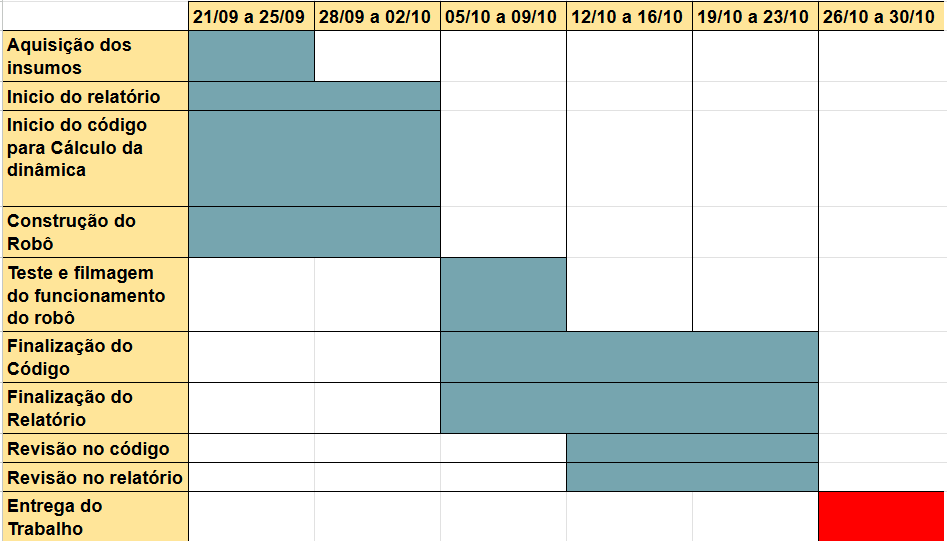
\includegraphics[width=13cm]{gantt.png}
\caption{\label{fig:gantt}- Diagrama de Gantt com o cronograma de atividades do projeto.}
\end{center}
\end{figure}

\section{Organização do Trabalho}

O Capítulo \ref{chapter:revisao} apresenta a fundamentação teórica: a cinemática e a cinética do corpo rígido, o tensor de inércia e o equacionamento de um sistema de corpos. O Capítulo \ref{chapter:metodologia} descreve a construção do protótipo e o levantamento das massas e das dimensões. O Capítulo \ref{chapter:inercia} reúne o cálculo dos tensores de inércia de cada peça e do robô montado. O Capítulo \ref{chapter:modelo} desenvolve o modelo cinemático e dinâmico, e o Capítulo \ref{chapter:resultados} apresenta e discute os resultados da simulação. Por fim, são apresentadas as conclusões e, no Apêndice \ref{ap:codigo}, a estrutura do código utilizado.

\chapter{REVISÃO BIBLIOGRÁFICA}
\label{chapter:revisao}

Para o correto equacionamento do mecanismo robótico desenvolvido, é necessário estabelecer as bases teóricas da mecânica clássica aplicadas a corpos rígidos. Este capítulo apresenta as formulações vetoriais da cinemática e da cinética, o tensor de inércia e o procedimento usado para obter as equações de movimento do conjunto de corpos, que serão utilizados para modelar o movimento do robô.

\section{\textbf{Cinemática do Corpo Rígido}}
\label{sec:cinematica}

A cinemática estuda a geometria do movimento sem considerar as forças que o causam. Para um corpo rígido em movimento geral no espaço, a velocidade e a aceleração de qualquer ponto $B$ podem ser determinadas a partir de um ponto de referência $A$ pertencente ao mesmo corpo, utilizando equações de movimento relativo.

\subsection{\underline{Campo de Velocidades}}
A velocidade de um ponto $B$ em relação a um referencial fixo é dada pela soma da velocidade de translação do ponto $A$ com a velocidade gerada pela rotação do corpo em torno de $A$. A equação vetorial da velocidade é expressa por:

\begin{equation}
    \vec{v}_B = \vec{v}_A + \vec{\omega} \times \vec{r}_{B/A} + \vec{v}_{rel}
    \label{eq:velocidade}
\end{equation}

Onde $\vec{v}_B$ e $\vec{v}_A$ são os vetores velocidade absoluta dos pontos $B$ e $A$; $\vec{\omega}$ é o vetor velocidade angular do corpo; $\vec{r}_{B/A}$ é o vetor posição de $B$ em relação a $A$; e $\vec{v}_{rel}$ é a velocidade relativa caso haja deslizamento em referenciais móveis (que para corpos rigidamente conectados, é nula).

\subsection{\underline{Campo de Acelerações}}
Derivando-se a Equação \ref{eq:velocidade} em relação ao tempo, obtém-se o campo de acelerações do corpo rígido, dado por:

\begin{equation}
    \vec{a}_B = \vec{a}_A + \vec{\alpha} \times \vec{r}_{B/A} + \vec{\omega} \times (\vec{\omega} \times \vec{r}_{B/A}) + 2\vec{\omega} \times \vec{v}_{rel} + \vec{a}_{rel}
    \label{eq:aceleracao}
\end{equation}

Nesta formulação, $\vec{\alpha}$ representa o vetor aceleração angular. O termo $\vec{\alpha} \times \vec{r}_{B/A}$ é a componente tangencial da aceleração relativa, enquanto $\vec{\omega} \times (\vec{\omega} \times \vec{r}_{B/A})$ representa a componente normal (centrípeta). Os termos envolvendo $\vec{v}_{rel}$ e $\vec{a}_{rel}$ correspondem à aceleração de Coriolis e à aceleração relativa, respectivamente.

\section{\textbf{Cinética: Equações de Newton-Euler}}
\label{sec:cinetica}

A cinética relaciona as forças e momentos atuantes no sistema com o movimento resultante. Para um corpo rígido espacial, essa relação é regida pelas equações de Newton-Euler. 

O somatório das forças externas atua sobre o centro de massa (CM) regendo sua translação:
\begin{equation}
    \sum \vec{F}_{ext} = m\vec{a}_{cm}
    \label{eq:newton}
\end{equation}

Para o movimento rotacional, o somatório dos momentos das forças externas em relação ao centro de massa ($\vec{M}_{fe/*}$) é governado pela taxa de variação do momento angular. Na notação tensorial e em eixos solidários ao corpo, a equação de Euler é:

\begin{equation}
    \sum \vec{M}_{fe/*} = [I]\vec{\alpha} + \vec{\omega} \times ([I]\vec{\omega})
    \label{eq:euler_momentos}
\end{equation}

Onde $[I]$ é a matriz do tensor de inércia em relação ao centro de massa. O segundo termo do lado direito, $\vec{\omega} \times ([I]\vec{\omega})$, representa a parcela giroscópica não-linear inerente ao movimento rotacional no espaço 3D.
\section{\textbf{Tensor de Inércia}}
\label{sec:tensor}

A distribuição de massa de um corpo rígido em relação a um ponto $P$ é caracterizada pelo tensor de inércia, cujos elementos são
\begin{equation}
    I_{ij} = \int_V \left( r^{2}\,\delta_{ij} - r_i\,r_j \right) dm ,
    \label{eq:tensor}
\end{equation}
em que $r_i$ são as coordenadas do elemento de massa $dm$ em relação a $P$, $r^2=r_1^2+r_2^2+r_3^2$ e $\delta_{ij}$ é o delta de Kronecker. Os elementos da diagonal são os momentos de inércia e os elementos fora da diagonal são os produtos de inércia (com sinal trocado). O tensor é simétrico e sempre existe um sistema de eixos, os eixos principais, em que ele é diagonal; os elementos diagonais correspondentes são os momentos principais de inércia, autovalores de $[I]$.

Para sólidos homogêneos simples, com a origem no centro de massa e os eixos ao longo das direções de simetria, o tensor é diagonal e conhecido. Para um paralelepípedo de massa $m$ e arestas $a$, $b$ e $c$ ao longo de $x$, $y$ e $z$:
\begin{equation}
    [I^*_{par}] = \frac{m}{12}\,\mathrm{diag}\!\left(b^{2}+c^{2},\; a^{2}+c^{2},\; a^{2}+b^{2}\right),
    \label{eq:Ipar}
\end{equation}
e para um cilindro maciço de massa $m$, raio $r$ e altura $h$, com eixo ao longo de $z$:
\begin{equation}
    [I^*_{cil}] = \mathrm{diag}\!\left(\frac{m(3r^{2}+h^{2})}{12},\; \frac{m(3r^{2}+h^{2})}{12},\; \frac{m\,r^{2}}{2}\right).
    \label{eq:Icil}
\end{equation}
Esses dois sólidos são suficientes para representar todas as peças do robô: os palitos e a bateria como paralelepípedos, e o pino, o furo e o eixo do motor como cilindros.

\section{\textbf{Teorema dos Eixos Paralelos e Composição de Corpos}}
\label{sec:composicao}

Se $[I^*]$ é o tensor de uma peça em relação ao seu centro de massa e $\vec d$ é o vetor que vai do ponto de referência $P$ ao centro de massa da peça, o tensor em relação a $P$ é, na forma tensorial do teorema dos eixos paralelos (Steiner),
\begin{equation}
    [I_P] = [I^*] + m\left( |\vec d|^{2}\,[\mathbb{I}] - \vec d\,\vec d^{\,T} \right).
    \label{eq:steiner}
\end{equation}
Uma peça descrita em um sistema próprio, girada em relação ao sistema do corpo por uma matriz de rotação $[R]$, tem tensor $[R][I^*][R]^T$ no sistema do corpo. Um corpo composto por $n$ peças, de massas $m_i$ e centros de massa em $\vec r_i$, tem massa $m=\sum m_i$, centro de massa $\vec r_{cm}=\sum m_i\vec r_i/m$ e tensor em torno do seu centro de massa
\begin{equation}
    [I^*_{cj}] = \sum_{i=1}^{n}\left\{ [R_i][I^*_i][R_i]^T + m_i\left( |\vec d_i|^{2}\,[\mathbb{I}] - \vec d_i\,\vec d_i^{\,T}\right)\right\},
    \qquad \vec d_i=\vec r_i-\vec r_{cm}.
    \label{eq:composicao}
\end{equation}
Furos e cavidades são tratados como peças de massa negativa. No movimento plano em torno de um eixo paralelo a $z$ que passa por um pivô a uma distância $d$ do centro de massa, o momento de inércia reduz-se a $I_{piv\hat{o}}=I^*_{zz}+m\,d^{2}$.

\section{\textbf{Equações de Movimento de um Sistema de Corpos}}
\label{sec:sistemas}

Em um sistema de corpos rígidos descrito por coordenadas generalizadas $q_k$, cada corpo $i$ satisfaz as equações de Newton e de Euler (Equações \ref{eq:newton} e \ref{eq:euler_momentos}), mas as forças de ligação entre os corpos são incógnitas. Chamando de velocidades parciais as derivadas $\vec v_i^{\,k}=\partial\vec v_i/\partial\dot q_k$ e $\vec\omega_i^{\,k}=\partial\vec\omega_i/\partial\dot q_k$, a projeção das equações de Newton e de Euler sobre essas direções elimina as reações de ligação que não realizam trabalho, o que é a essência do método de Kane \cite{kane1985}. As equações de movimento resultam, para cada coordenada generalizada,
\begin{equation}
    \sum_i\left[\left(m_i\vec a_i-\vec F_i\right)\cdot\vec v_i^{\,k}+\left(\frac{d\vec H_i}{dt}-\vec M_i\right)\cdot\vec\omega_i^{\,k}\right]=0 ,
    \label{eq:kane_rev}
\end{equation}
em que $d\vec H_i/dt=[I_i]\vec\alpha_i+\vec\omega_i\times([I_i]\vec\omega_i)$ é o lado direito da Equação \ref{eq:euler_momentos}. Os livros de Dinâmica \cite{meriam2012,hibbeler2016,beer2013} tratam a obtenção dessas equações pelas leis de Newton-Euler e por princípios de trabalho virtual; a Equação \ref{eq:kane_rev} é equivalente às equações de Lagrange.

Quando há uma ligação com o ambiente, como um gancho preso a um ponto da corda, ela é imposta por uma restrição $\mathbf g(\mathbf q,t)=\mathbf 0$ e por multiplicadores de Lagrange $\boldsymbol\lambda$, que representam as forças de contato. A derivação da restrição em relação ao tempo fornece uma equação linear nas acelerações, que, acrescentada às equações de movimento, forma um sistema algébrico para $\ddot{\mathbf q}$ e $\boldsymbol\lambda$ (Seção \ref{sec:contato}). Para que a restrição não se degrade na integração numérica, usa-se a estabilização de Baumgarte \cite{baumgarte1972}. Quando uma nova restrição é imposta de forma abrupta, o contato é tratado como um impacto perfeitamente plástico, no qual o impulso das forças de contato altera as velocidades generalizadas sem alterar as posições.

\chapter{MODELAGEM FÍSICA E METODOLOGIA}
\label{chapter:metodologia}

Para validar a teoria matemática exposta no Capítulo \ref{chapter:revisao}, desenvolveu-se um protótipo físico articulado. Este capítulo descreve a construção mecânica do mecanismo robótico, apresentando a lista de insumos utilizados, as ferramentas aplicadas e a extração dos parâmetros geométricos de cada membro que compõe o sistema.

\section{Construção do Protótipo}
\label{sec:construcao}

A concepção física do mecanismo robótico foi inspirada em tutoriais e modelos educacionais de mecanismos articulados disponíveis no YouTube. O projeto foi adaptado para atender aos requisitos rigorosos de análise cinemática e cinética exigidos na disciplina de Dinâmica, garantindo que o movimento real do sistema pudesse ser descrito pelas equações vetoriais de Newton-Euler \cite{hibbeler2016}.

O foco da montagem foi a utilização de materiais de baixo custo e fácil manipulação, garantindo, ao mesmo tempo, a rigidez estrutural necessária para suportar os esforços gerados pelo acionamento do motor DC com redução.

A \ref{tab:quant_materiais} detalha o inventário de todos os componentes, insumos e ferramentas empregados na fabricação e montagem do protótipo robótico.

\begin{table}[H]
\centering
\caption{\label{tab:quant_materiais}- Relação quantitativa de materiais, insumos e ferramentas.}
\vspace*{.1cm}
\begin{tabular}{|l|c|c|}
\hline
\textbf{Item / Descrição} & \textbf{Categoria} & \textbf{Quantidade} \\
\hline
Palito de Picolé & Insumo (Estrutura) & 10 unidades \\ % Preencha a quantidade
\hline
Palito de Churrasco & Insumo (Eixos) & 03 unidades \\
\hline
Adesivo Instantâneo (Tekbond) & Insumo (Fixação) & 1 frasco \\
\hline
Cola Quente (Bastão) & Insumo (Preenchimento) & 01 unidades \\
\hline
Motor DC com Caixa de Redução & Componente Eletromecânico & 1 unidade \\
\hline
Bateria & Componente Eletromecânico & 1 unidade \\
\hline
Alicate de Corte & Ferramenta & 1 unidade \\
\hline
Micro Retífica & Ferramenta & 1 unidade \\
\hline
Paquímetro (resolução de 0,05 mm) & Instrumento de medição & 1 unidade \\
\hline
Balança de precisão & Instrumento de medição & 1 unidade \\
\hline
\end{tabular}
\end{table}

\subsection{Registro Fotográfico dos Insumos e Ferramentas}

A fim de documentar o processo de fabricação, as figuras a seguir ilustram individualmente cada um dos materiais e ferramentas listados na \ref{tab:quant_materiais}: os dois tipos de palito (\ref{fig:mat_picole} e \ref{fig:mat_churrasco}), o alicate para corte (\ref{fig:ferr_alicate}), a micro retífica para usinagem e furação (\ref{fig:ferr_retifica}) e o paquímetro usado nas medidas dimensionais (\ref{fig:ferr_paquimetro}).

\begin{figure}[H]
\begin{center}
 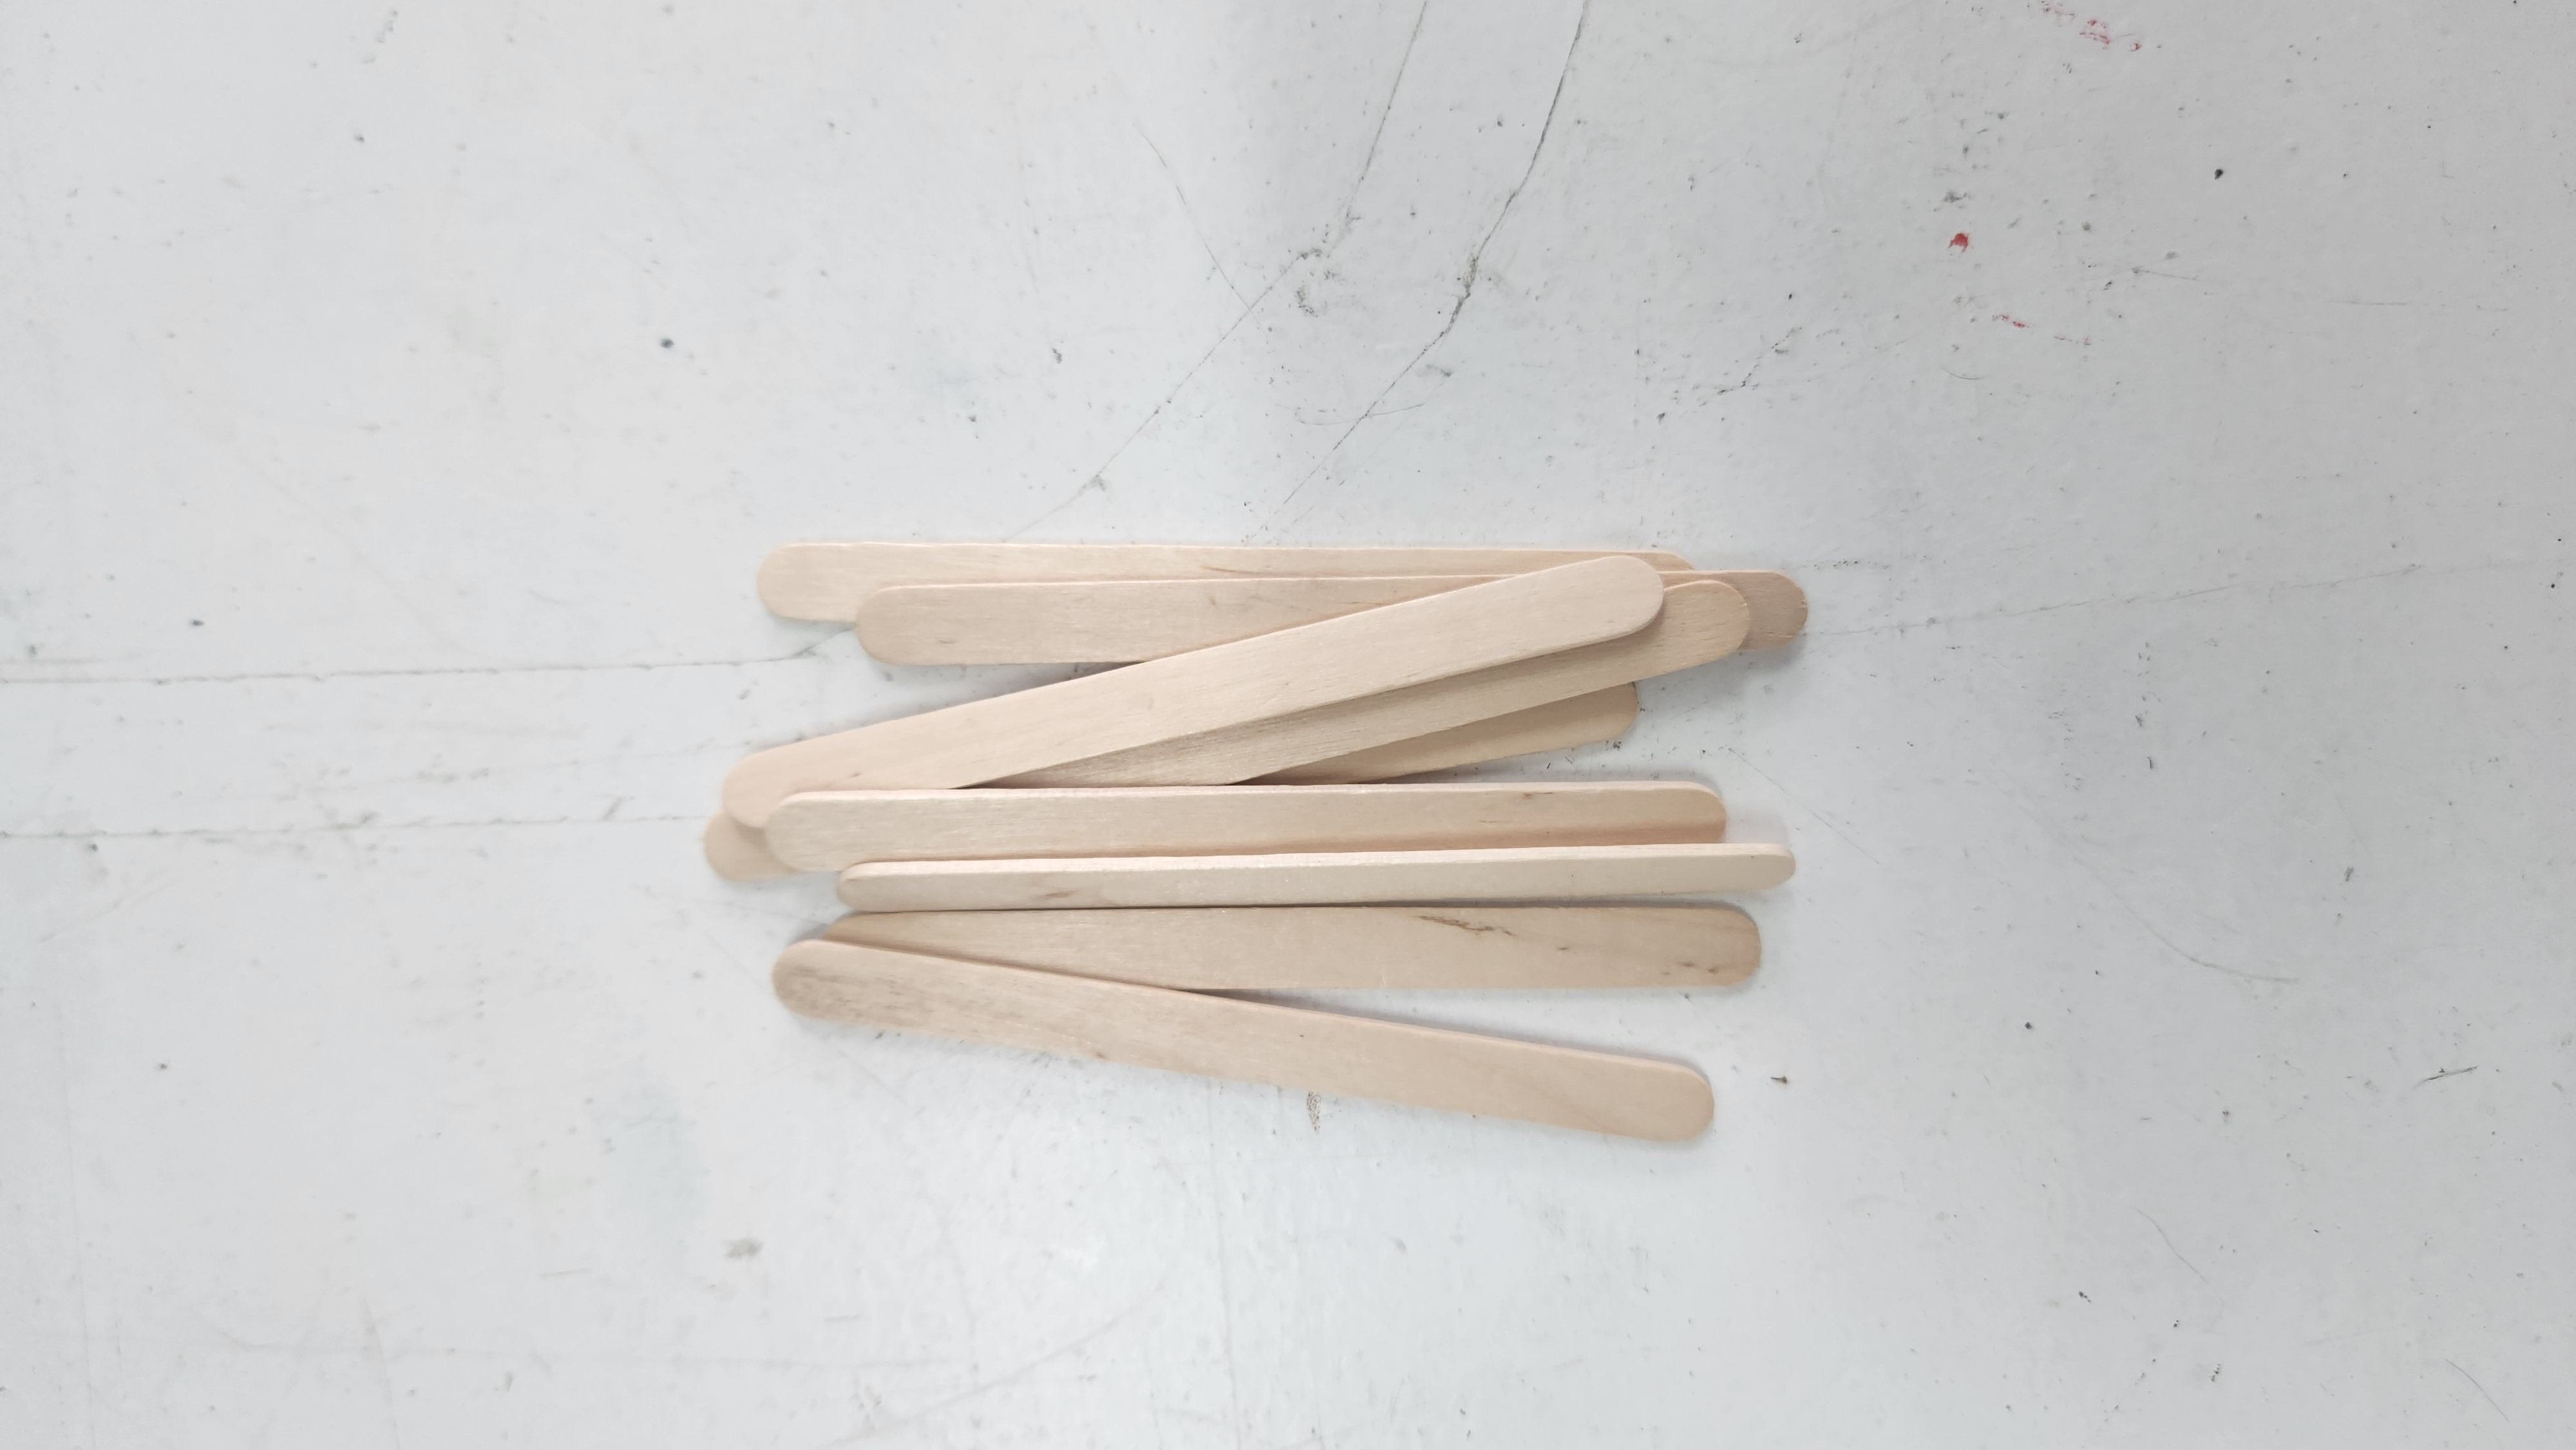
\includegraphics[width=12cm]{foto_palito_picole.jpg}
\caption{\label{fig:mat_picole}- Insumo estrutural: Palitos de picolé.}
\end{center}
\end{figure}

\begin{figure}[H]
\begin{center}
 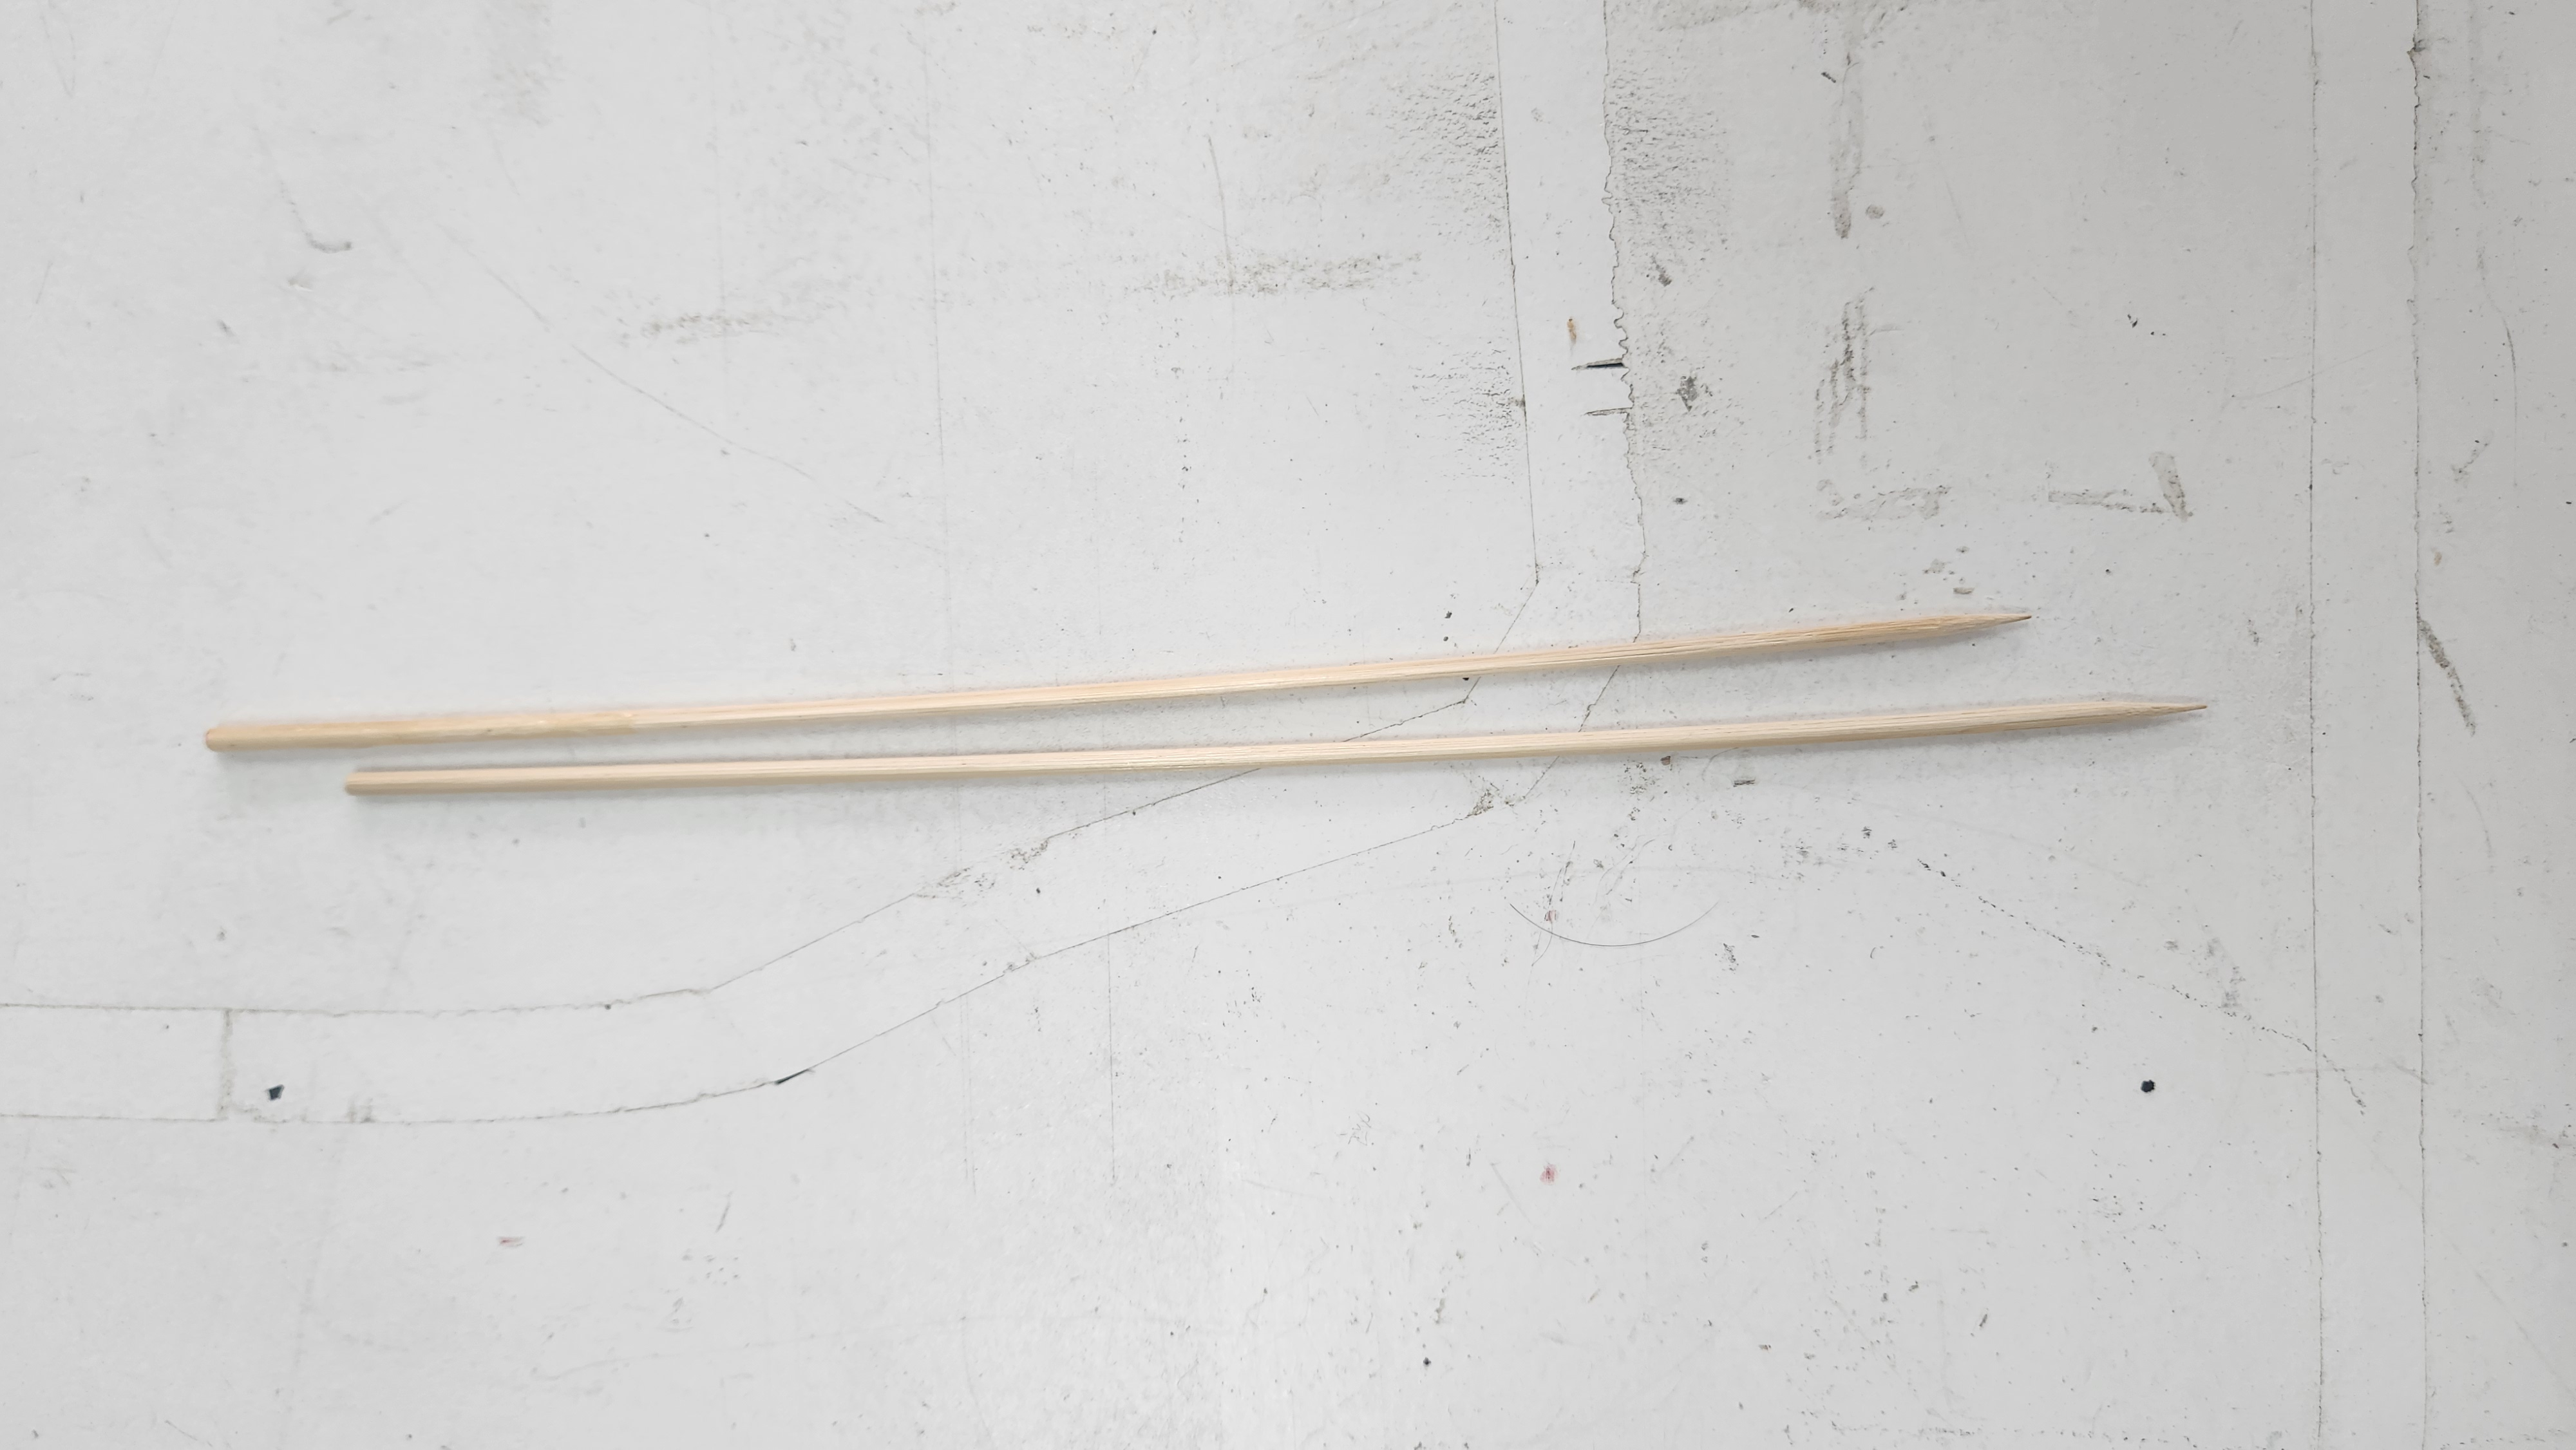
\includegraphics[width=12cm]{foto_palito_churrasco.jpg}
\caption{\label{fig:mat_churrasco}- Insumo para eixos de articulação: Palitos de churrasco.}
\end{center}
\end{figure}



\begin{figure}[H]
\begin{center}
 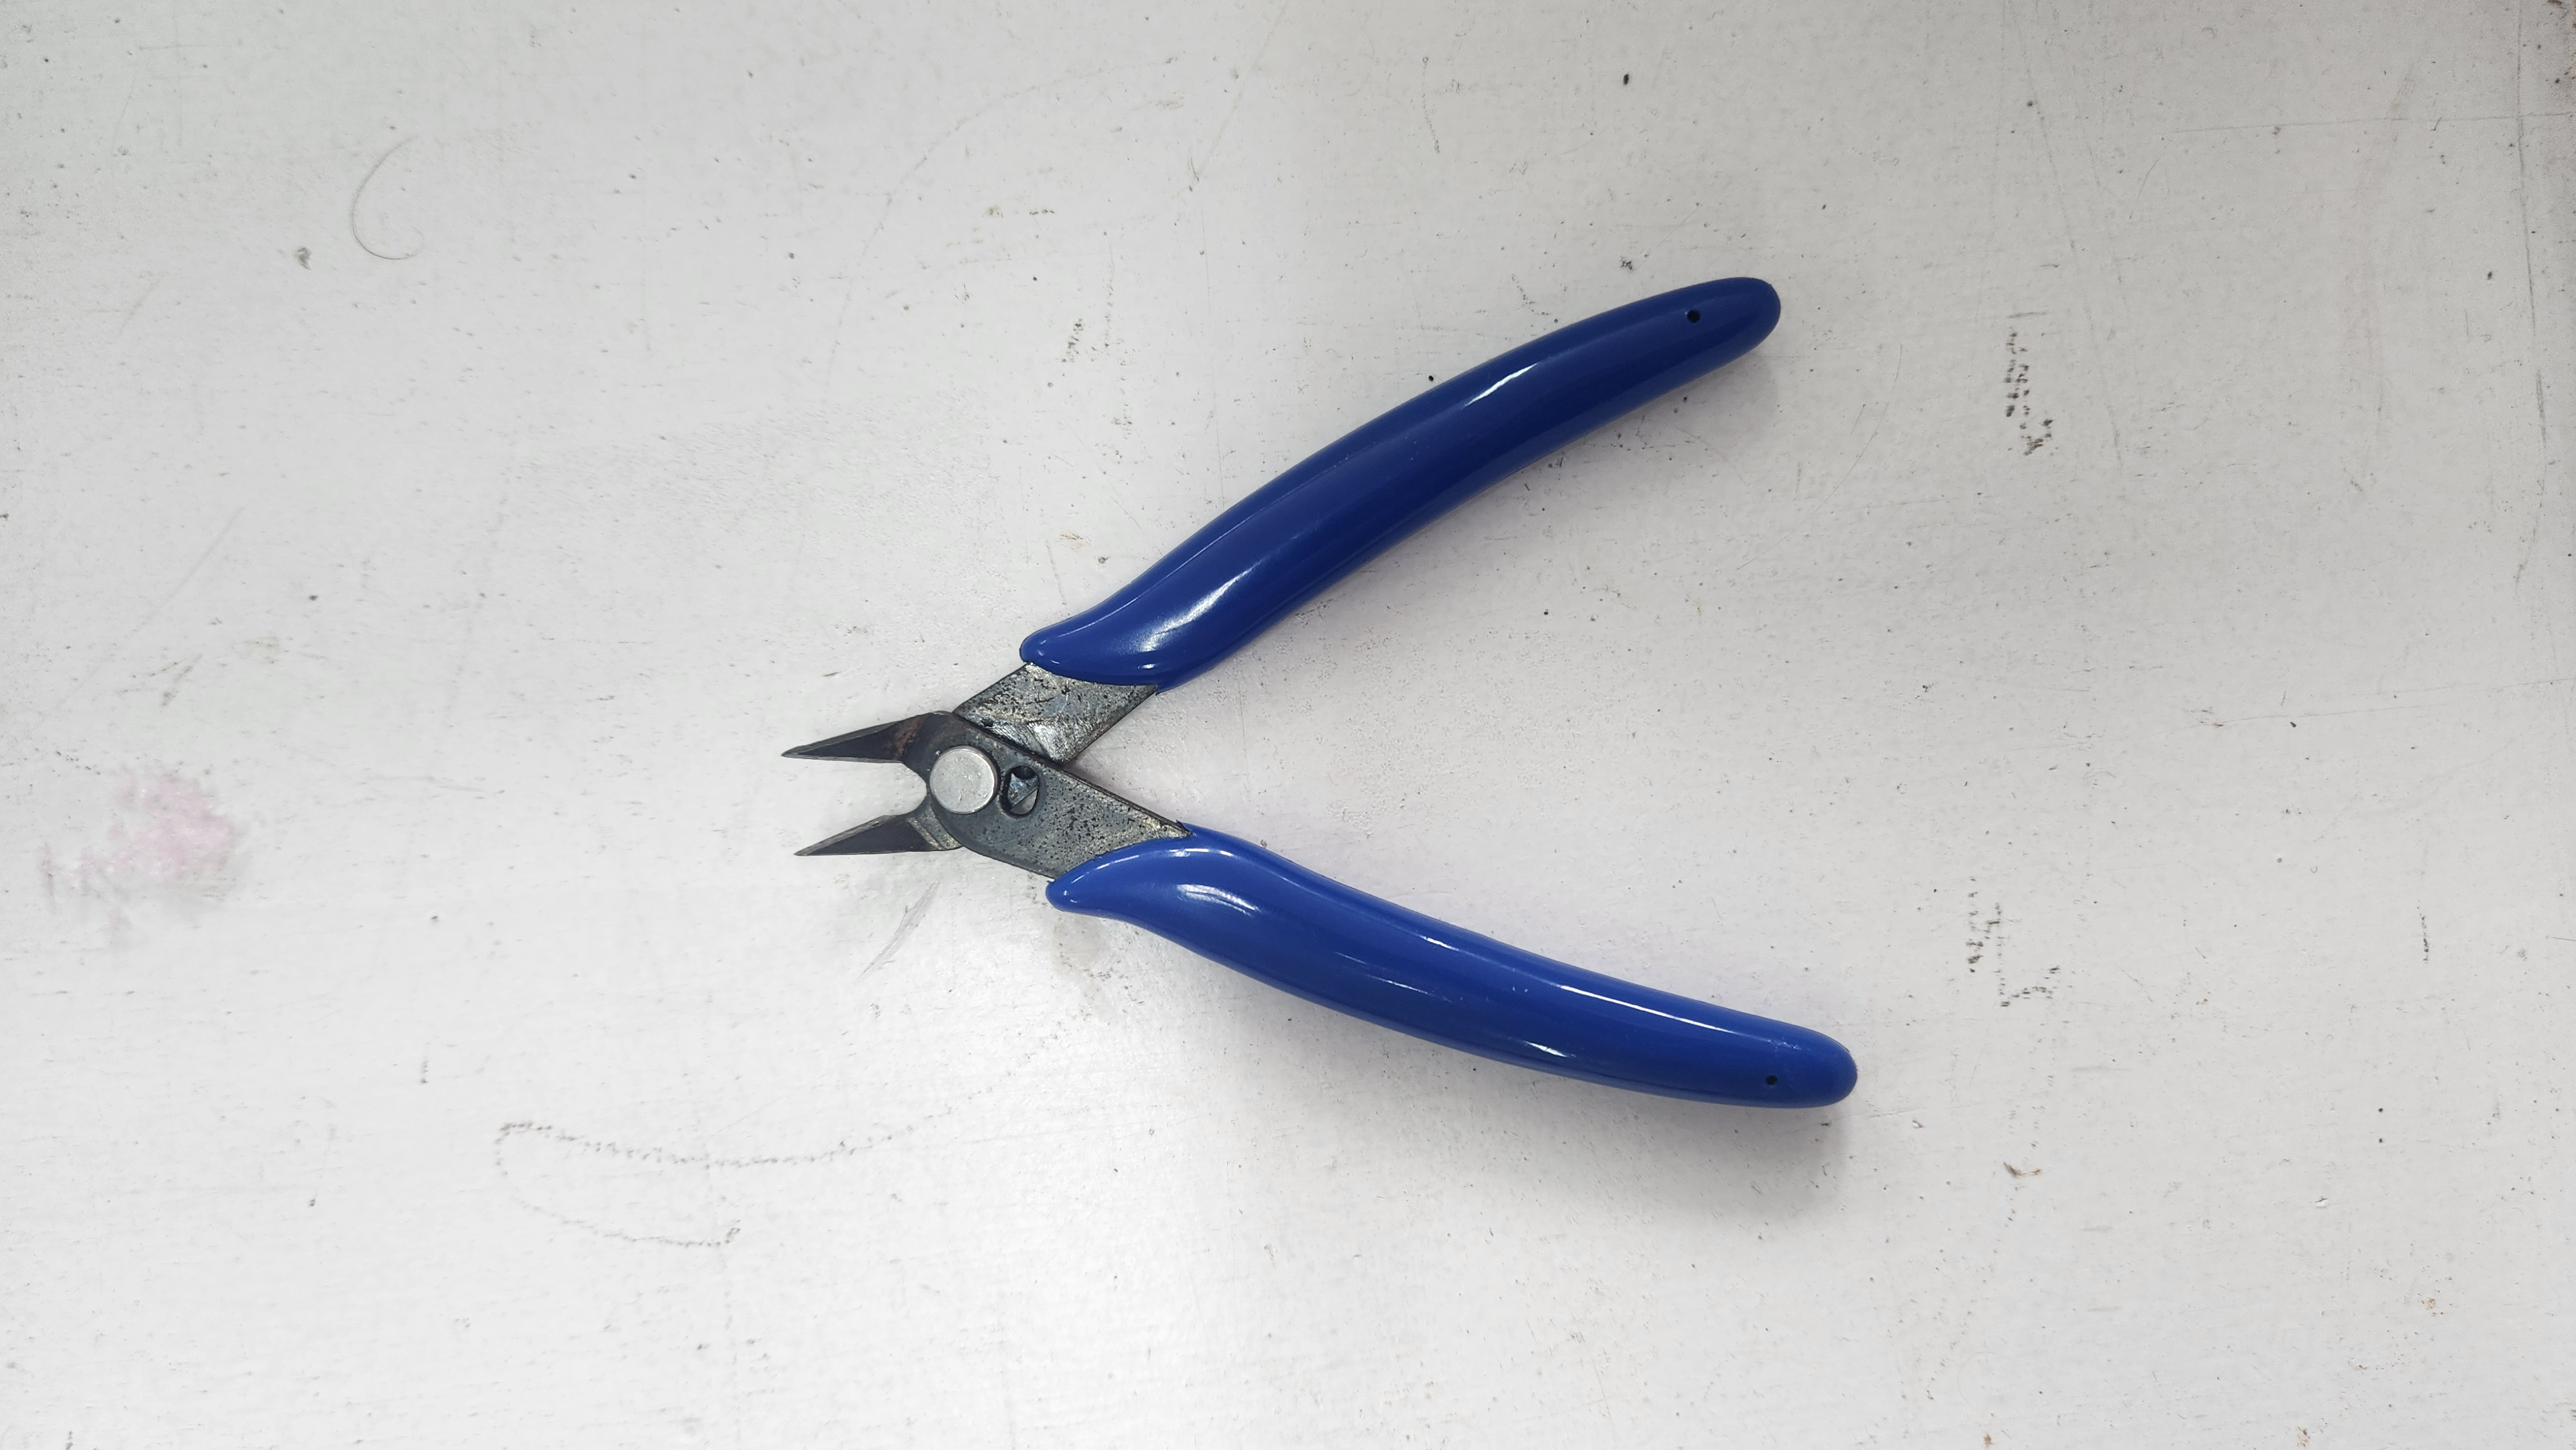
\includegraphics[width=12cm]{foto_alicate.jpg}
\caption{\label{fig:ferr_alicate}- Ferramenta de corte: Alicate.}
\end{center}
\end{figure}

\begin{figure}[H]
\begin{center}
 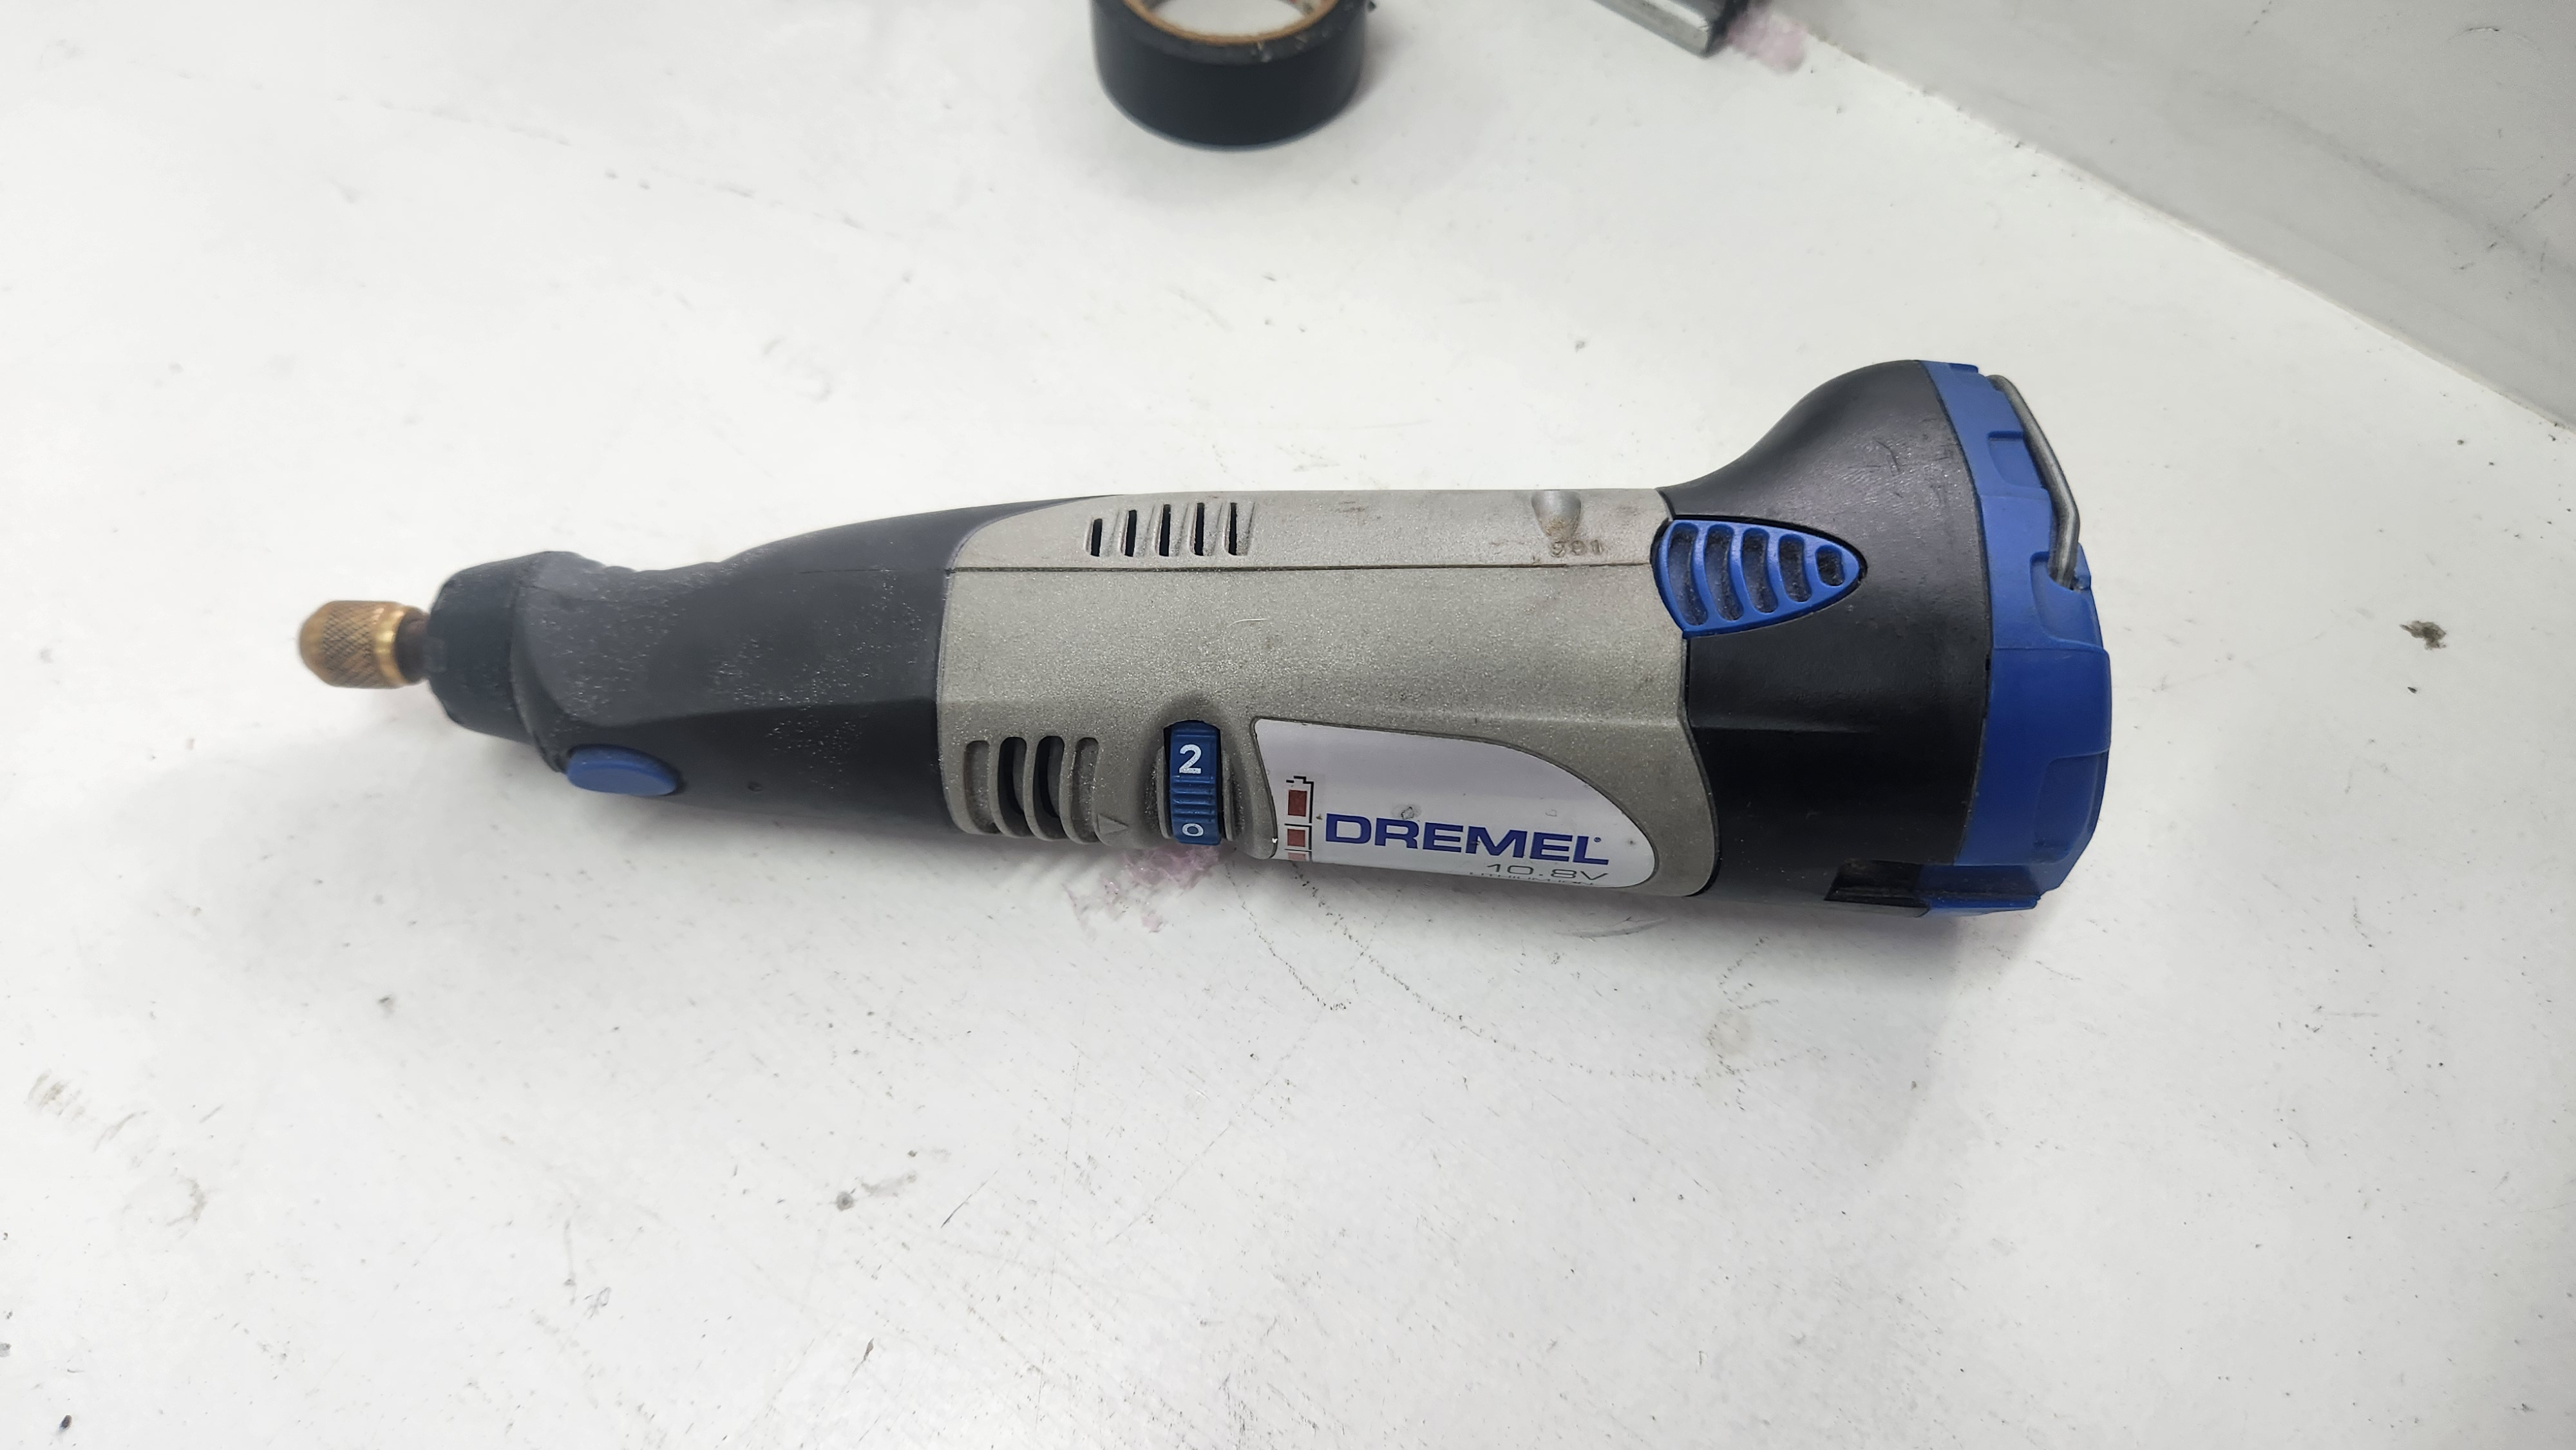
\includegraphics[width=12cm]{foto_retifica.jpg}
\caption{\label{fig:ferr_retifica}- Ferramenta de usinagem e furação: Micro retífica.}
\end{center}
\end{figure}

\begin{figure}[H]
\begin{center}
 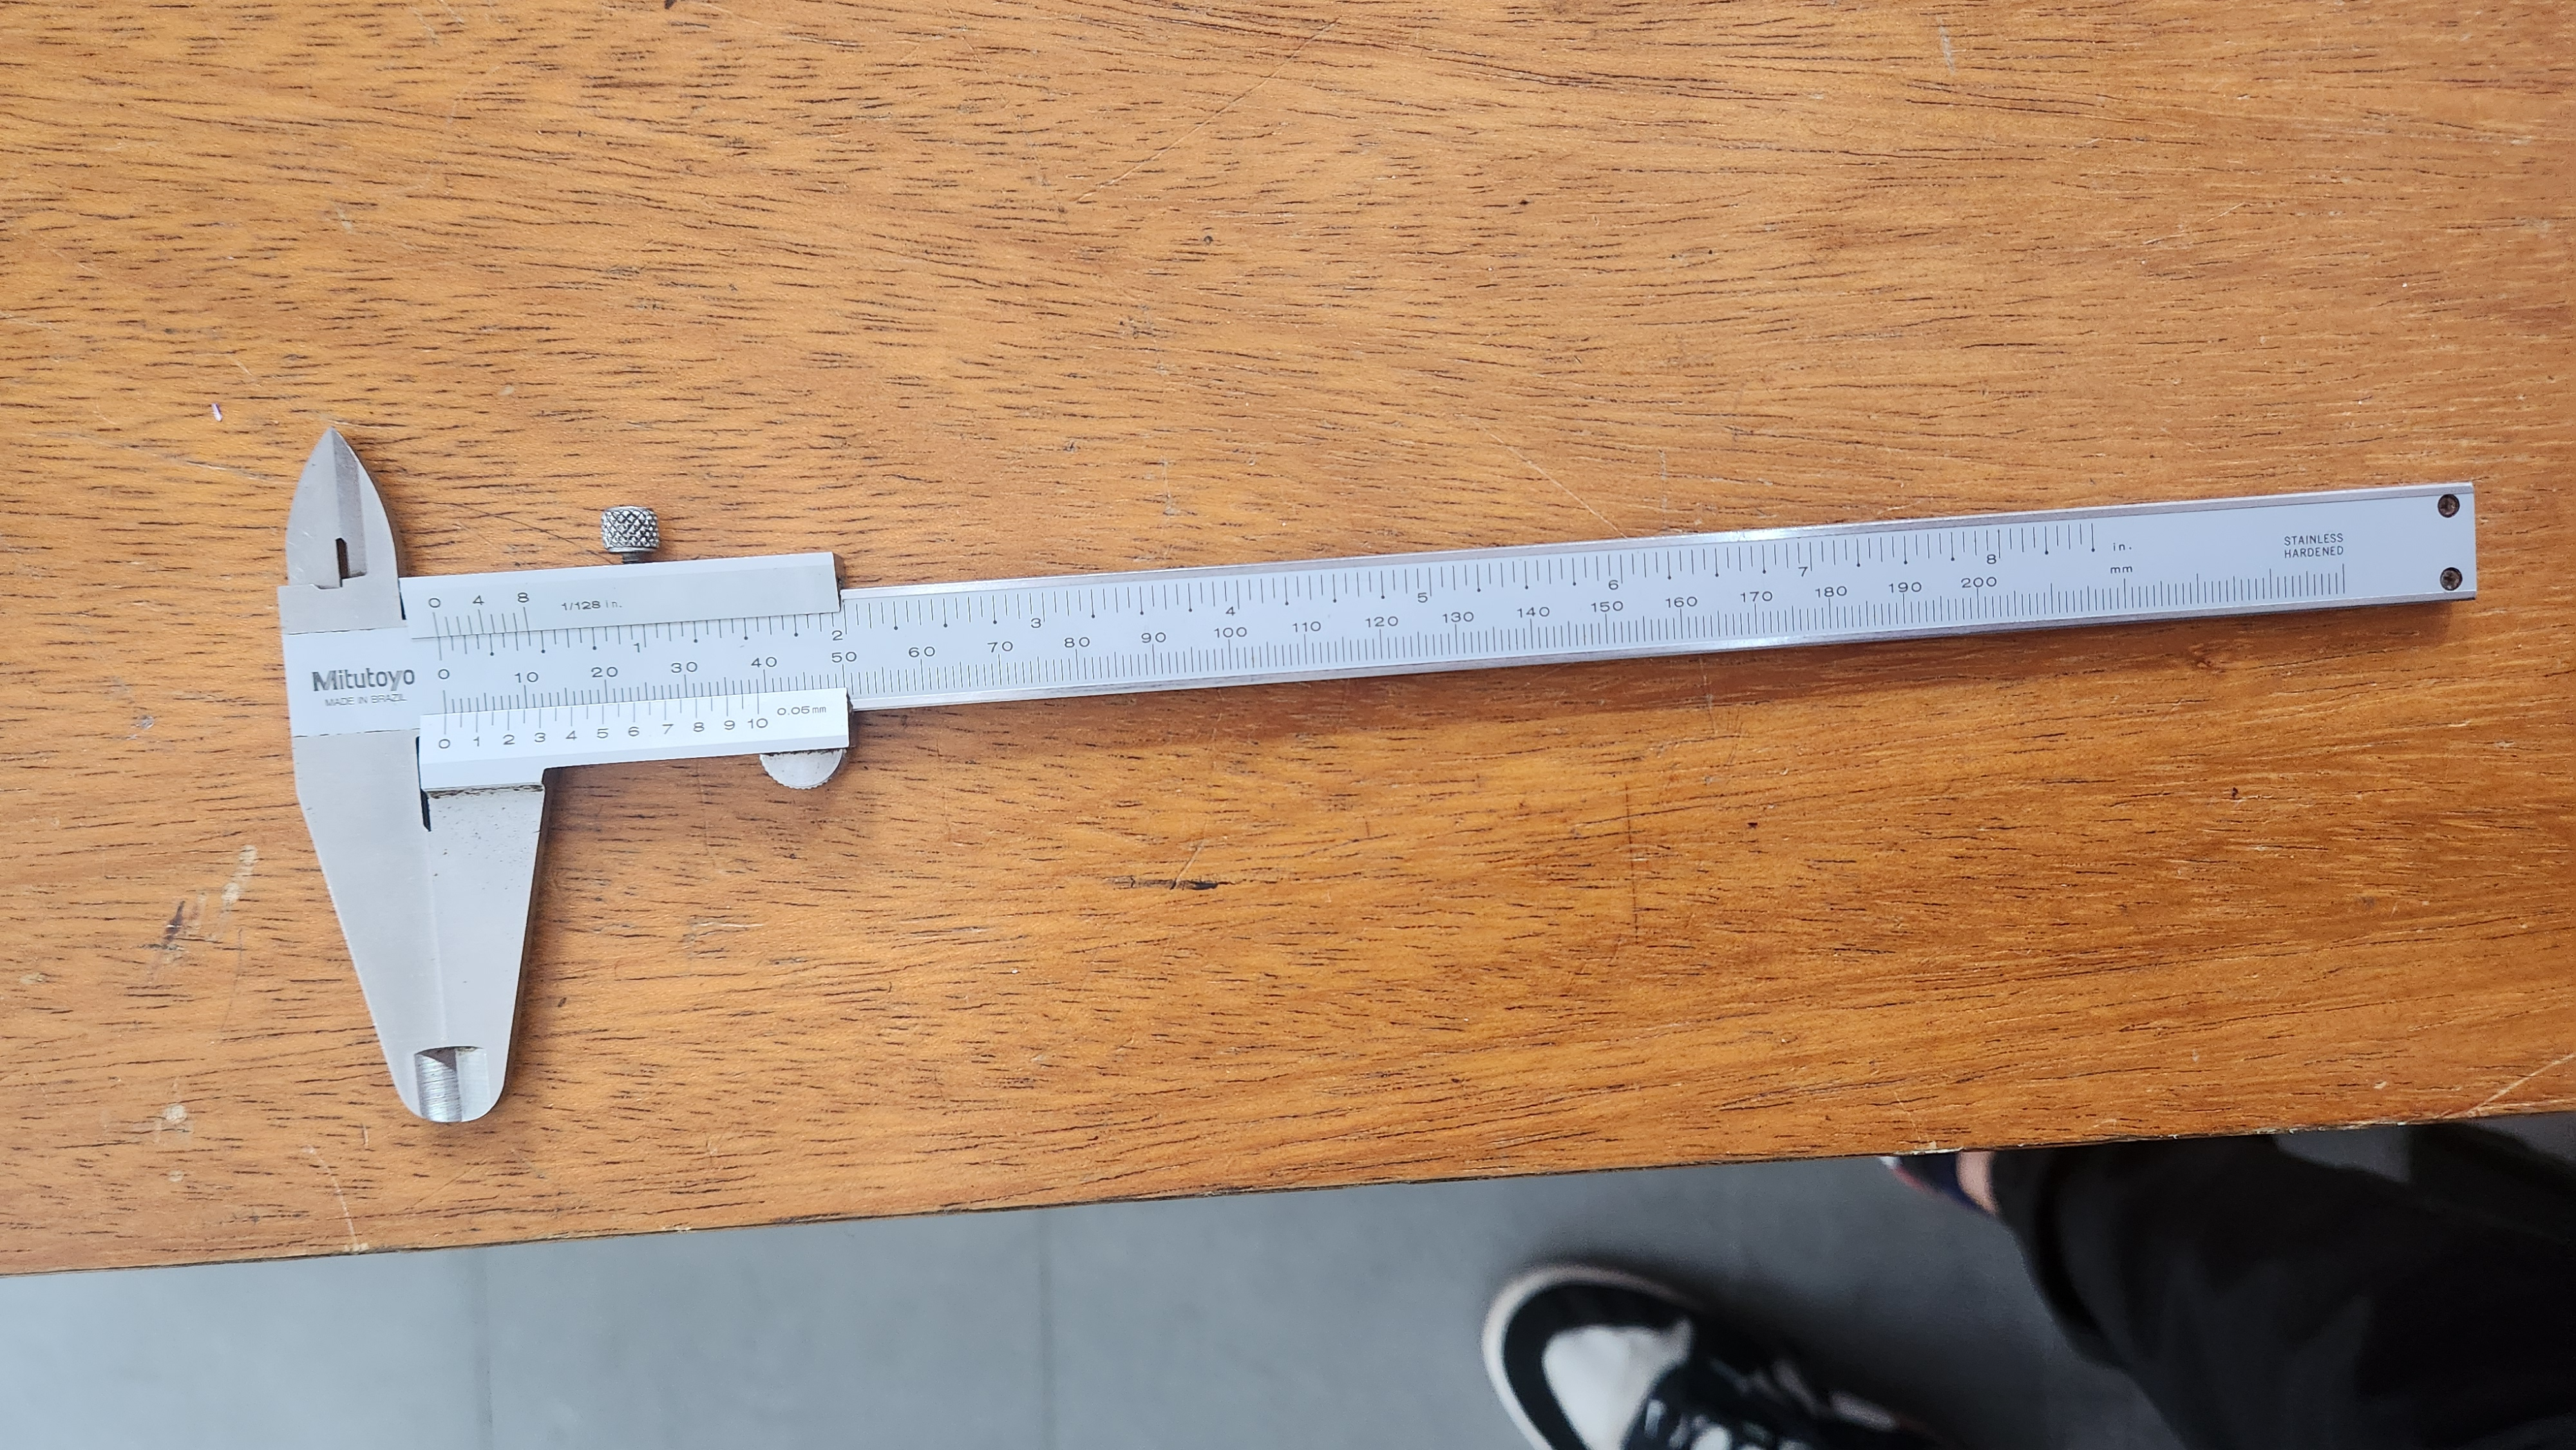
\includegraphics[width=12cm]{20261006_123529.jpg}
\caption{\label{fig:ferr_paquimetro}- Instrumento de medição: Paquímetro, de resolução de 0,05 mm, utilizado nas medidas lineares. As massas foram medidas com balança de precisão.}
\end{center}
\end{figure}

\section{Parâmetros Geométricos e Inerciais das Peças}
\label{sec:parametros}

A exatidão do modelo dinâmico depende diretamente das propriedades físicas de cada corpo rígido que compõe o mecanismo. O robô apresenta simetria em grande parte de sua estrutura, sendo subdividido analiticamente em 4 conjuntos de peças de madeira (Ombro, Quadril, Braço e Perna), aos quais se somam o motor com caixa de redução e a bateria, que formam o chassi. 

Para a aplicação das equações de movimento, levantou-se a massa individual de cada componente utilizando uma balança de precisão. Esses valores são fundamentais para o cálculo dos centros de massa e do tensor de inércia, e estão consolidados na \ref{tab:pesos_partes}. A massa da bateria foi medida; a do motor com caixa de redução foi medida em 26,6 g.

\begin{table}[H]
\centering
\caption{\label{tab:pesos_partes}- Massa individual das partes constituintes do robô.}
\vspace*{.1cm}
\begin{tabular}{|c|l|c|}
\hline
\textbf{Ref. Visual} & \textbf{Descrição do Componente} & \textbf{Massa (g)}\\
\hline
Fig. 1 e 2 & Ombro & 0,83 \\ 
\hline
Fig. 3 & Quadril & 0,81 \\
\hline
Fig. 4 & Braço & 2,0 \\
\hline
Fig. 5 e 6 & Perna & 1,5 \\
\hline
Fig. \ref{fig:desenho_motor} & Motor com caixa de redução (massa medida) & 26,6 \\
\hline
--- & Bateria & 67,03 \\
\hline
\end{tabular}
\end{table}

\subsection{Detalhamento Físico das Partes Móveis}

Além das massas, os comprimentos efetivos de cada elo foram medidos para a definição exata dos vetores posição ($\vec{r}_{B/A}$) utilizados nas equações cinemáticas. Devido à geometria 3D das peças, algumas exigiram documentação em mais de um plano. A seguir, são apresentadas as fotografias detalhadas das partes isoladas, evidenciando suas respectivas cotas dimensionais nas visões lateral e frontal.

\begin{figure}[H]
\begin{center}
 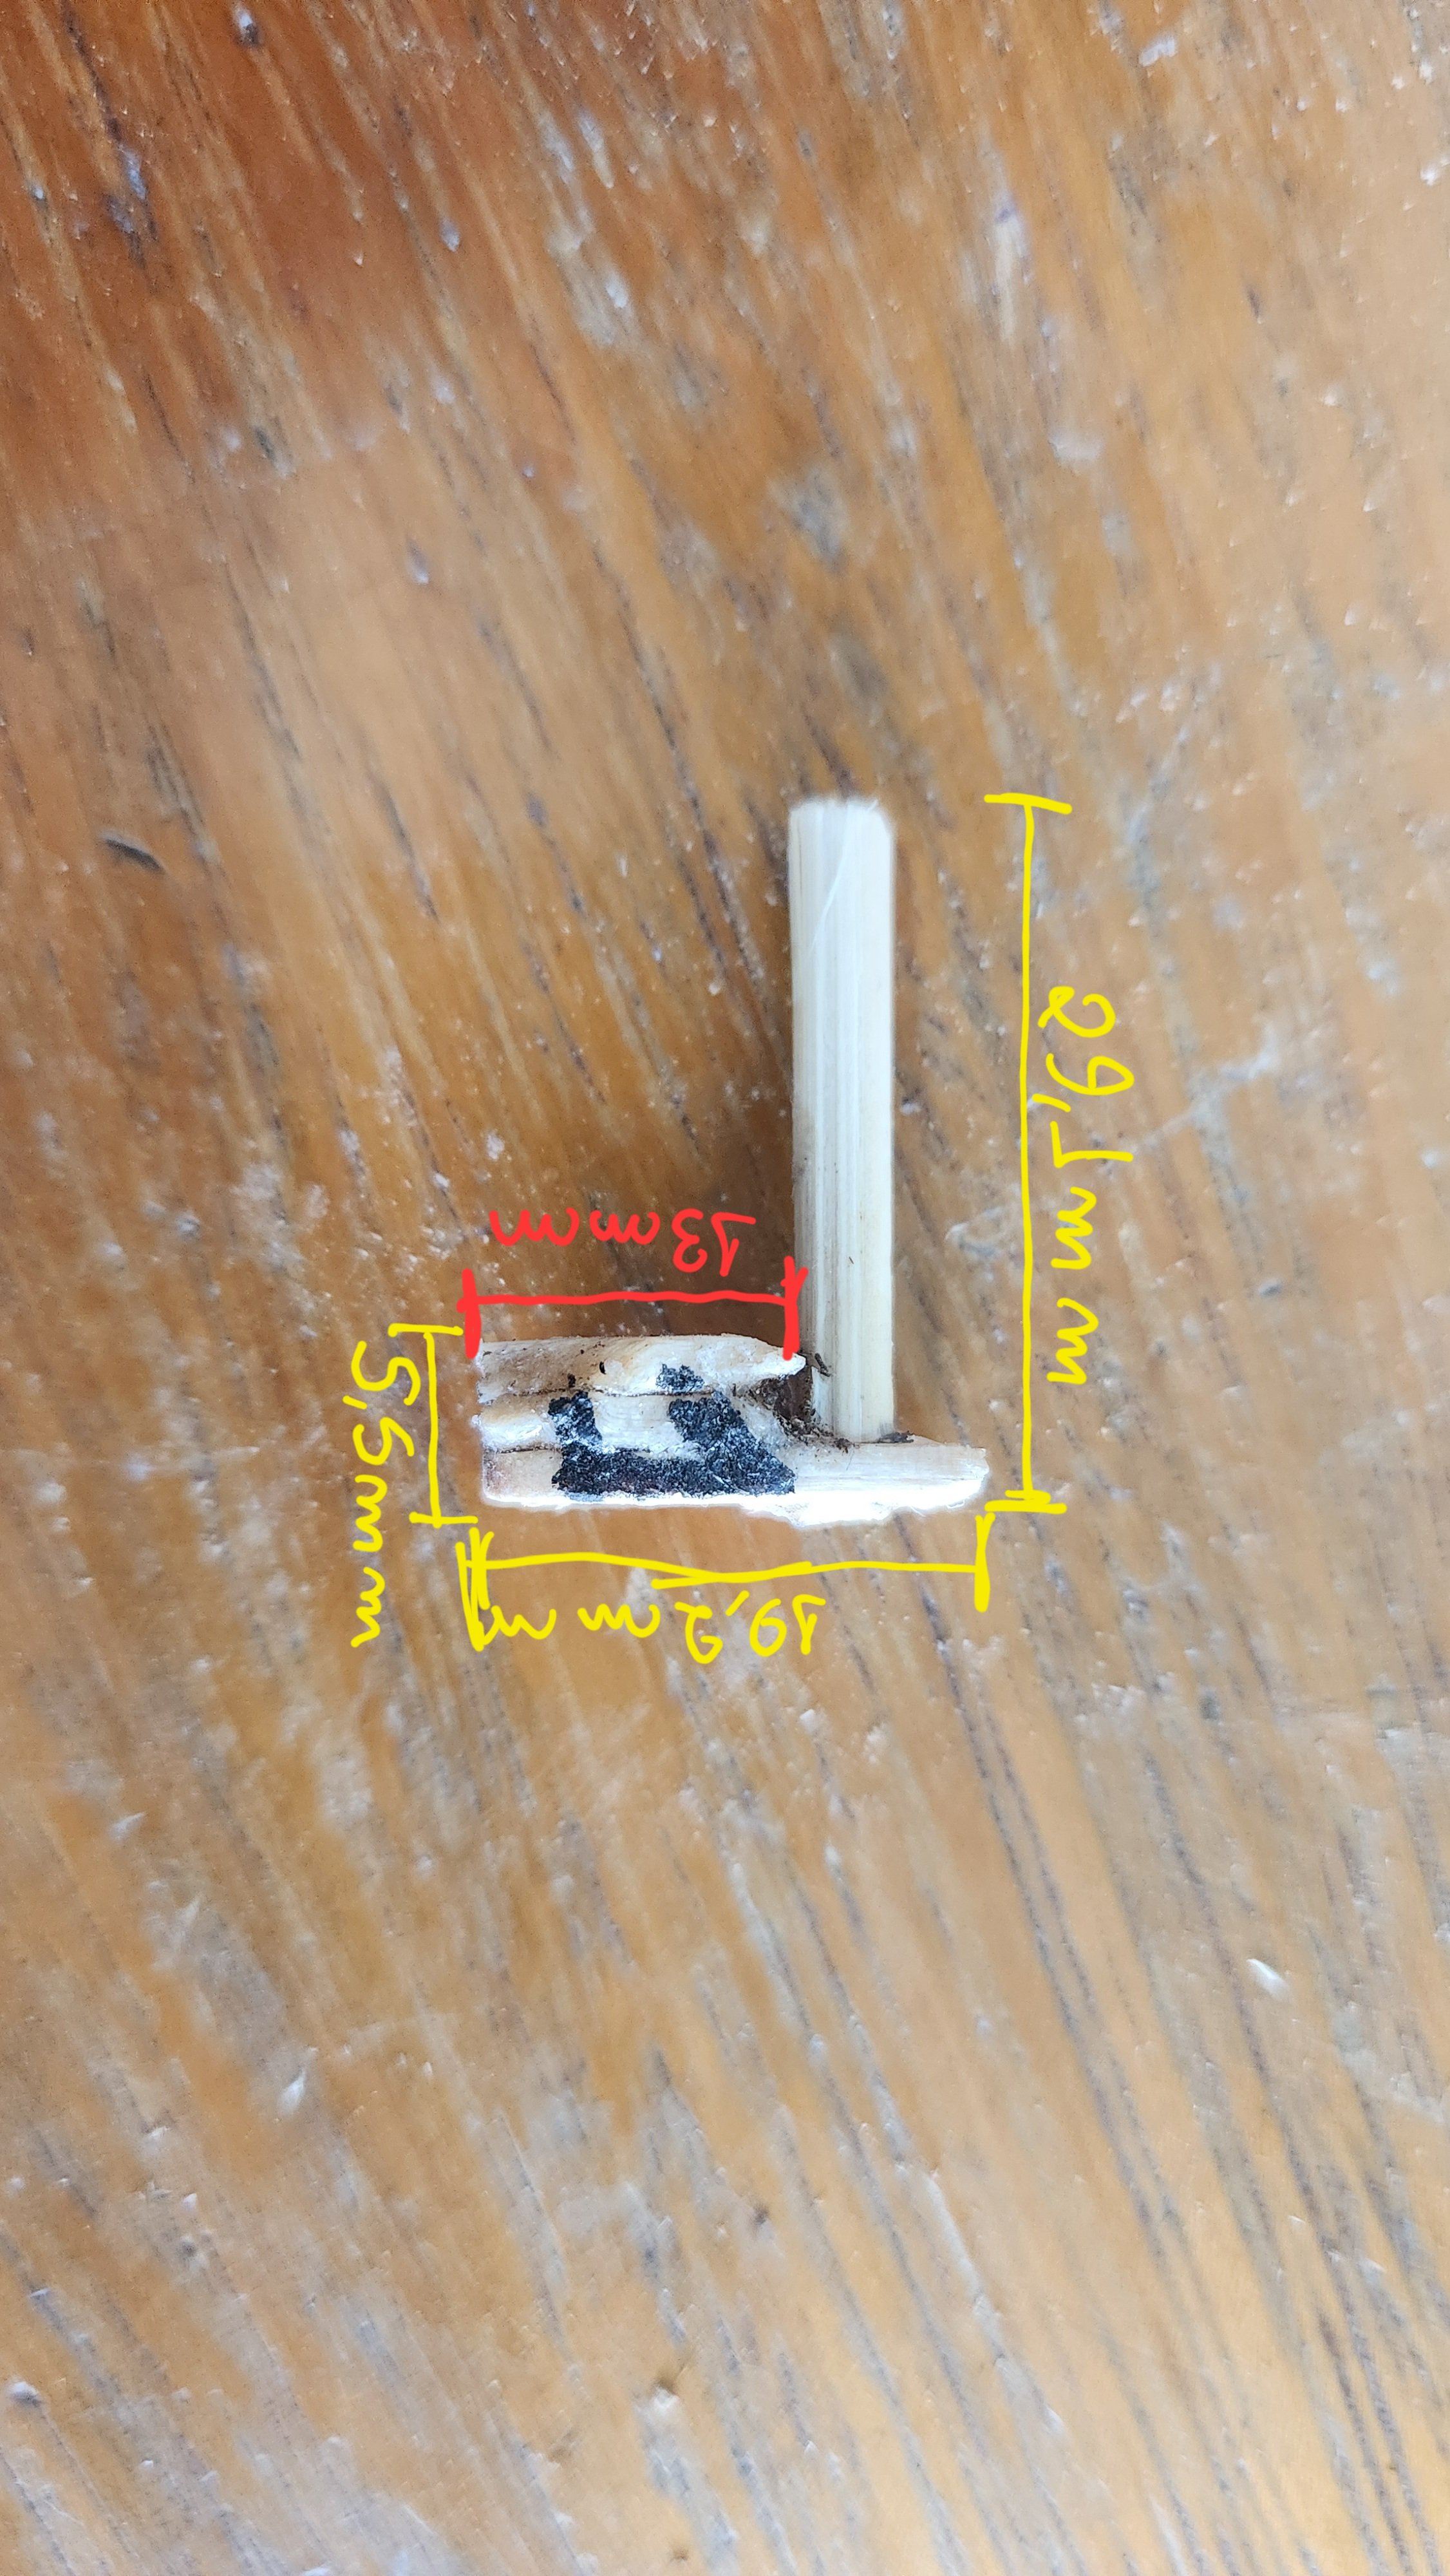
\includegraphics[width=10cm]{foto_parte1.jpg} % Lembre-se de ajustar o caminho da pasta se necessário, ex: ./03_Cap2/foto_parte1.jpg
\caption{\label{fig:parte1}- Detalhe e dimensões do Ombro (visão lateral).}
\end{center}
\end{figure}

\begin{figure}[H]
\begin{center}
 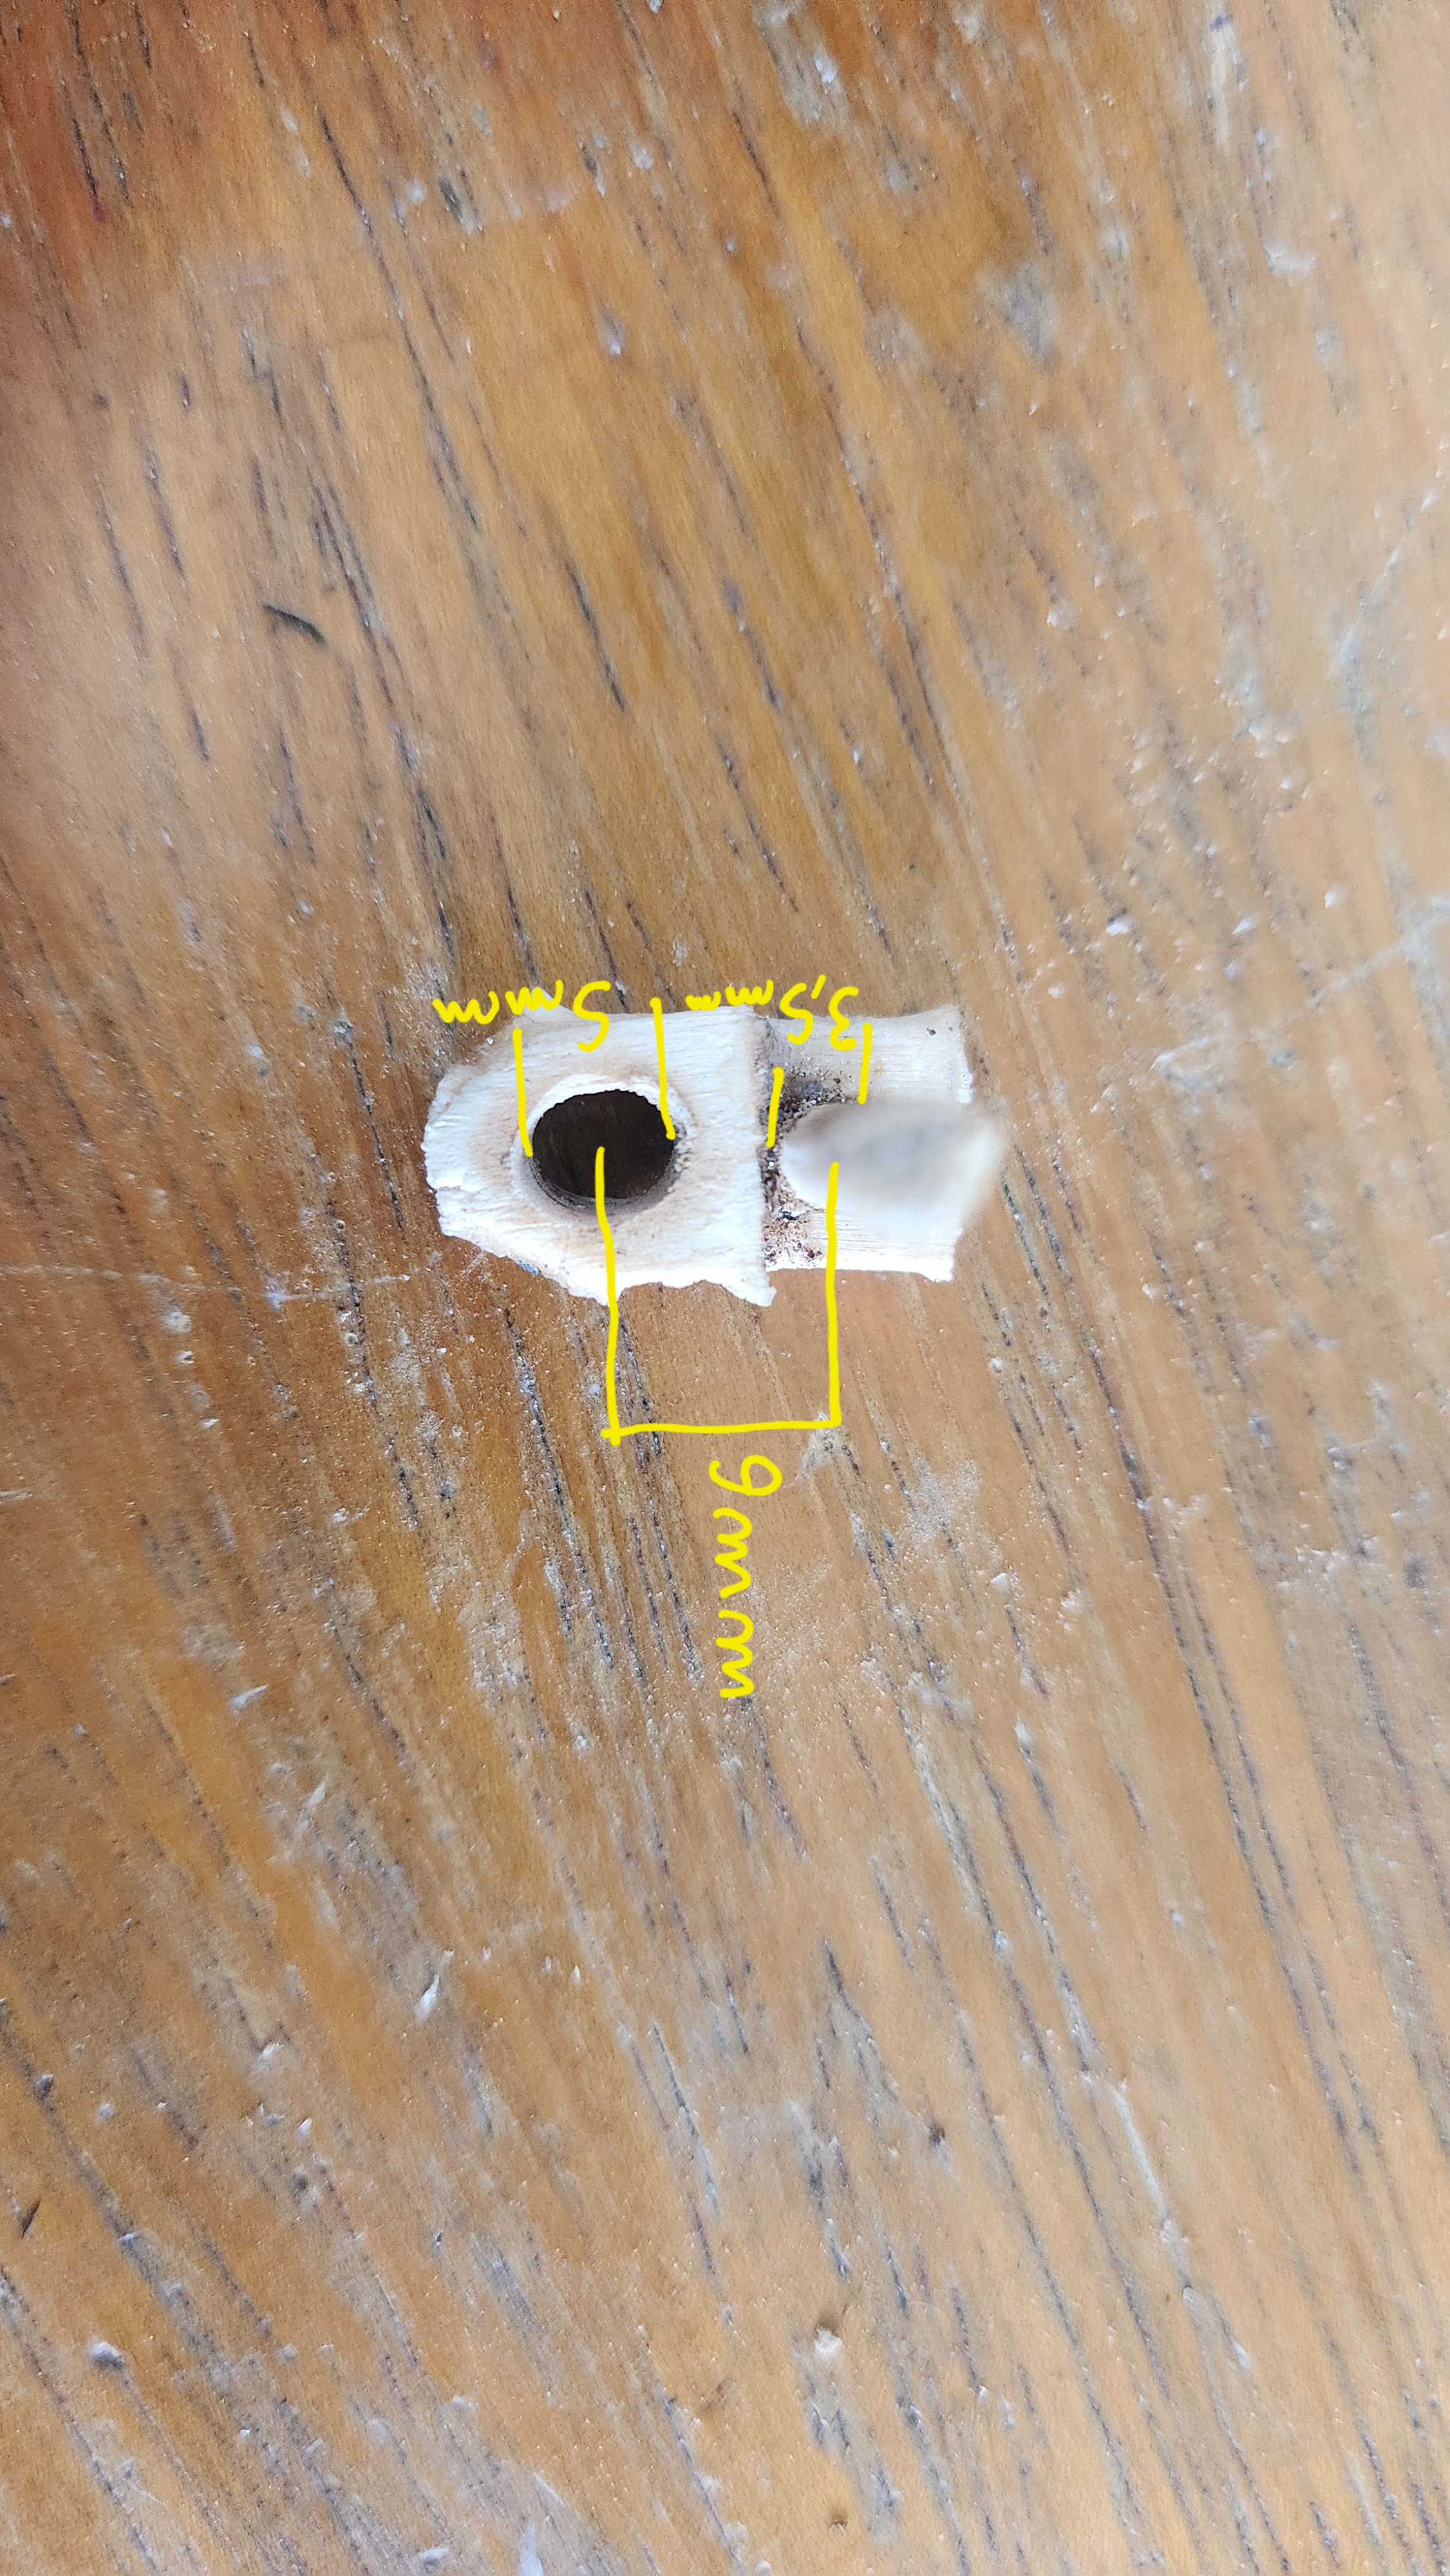
\includegraphics[width=10cm]{foto_parte2.jpg}
\caption{\label{fig:parte2}- Detalhe e dimensões do Ombro (visão frontal).}
\end{center}
\end{figure}

\begin{figure}[H]
\begin{center}
 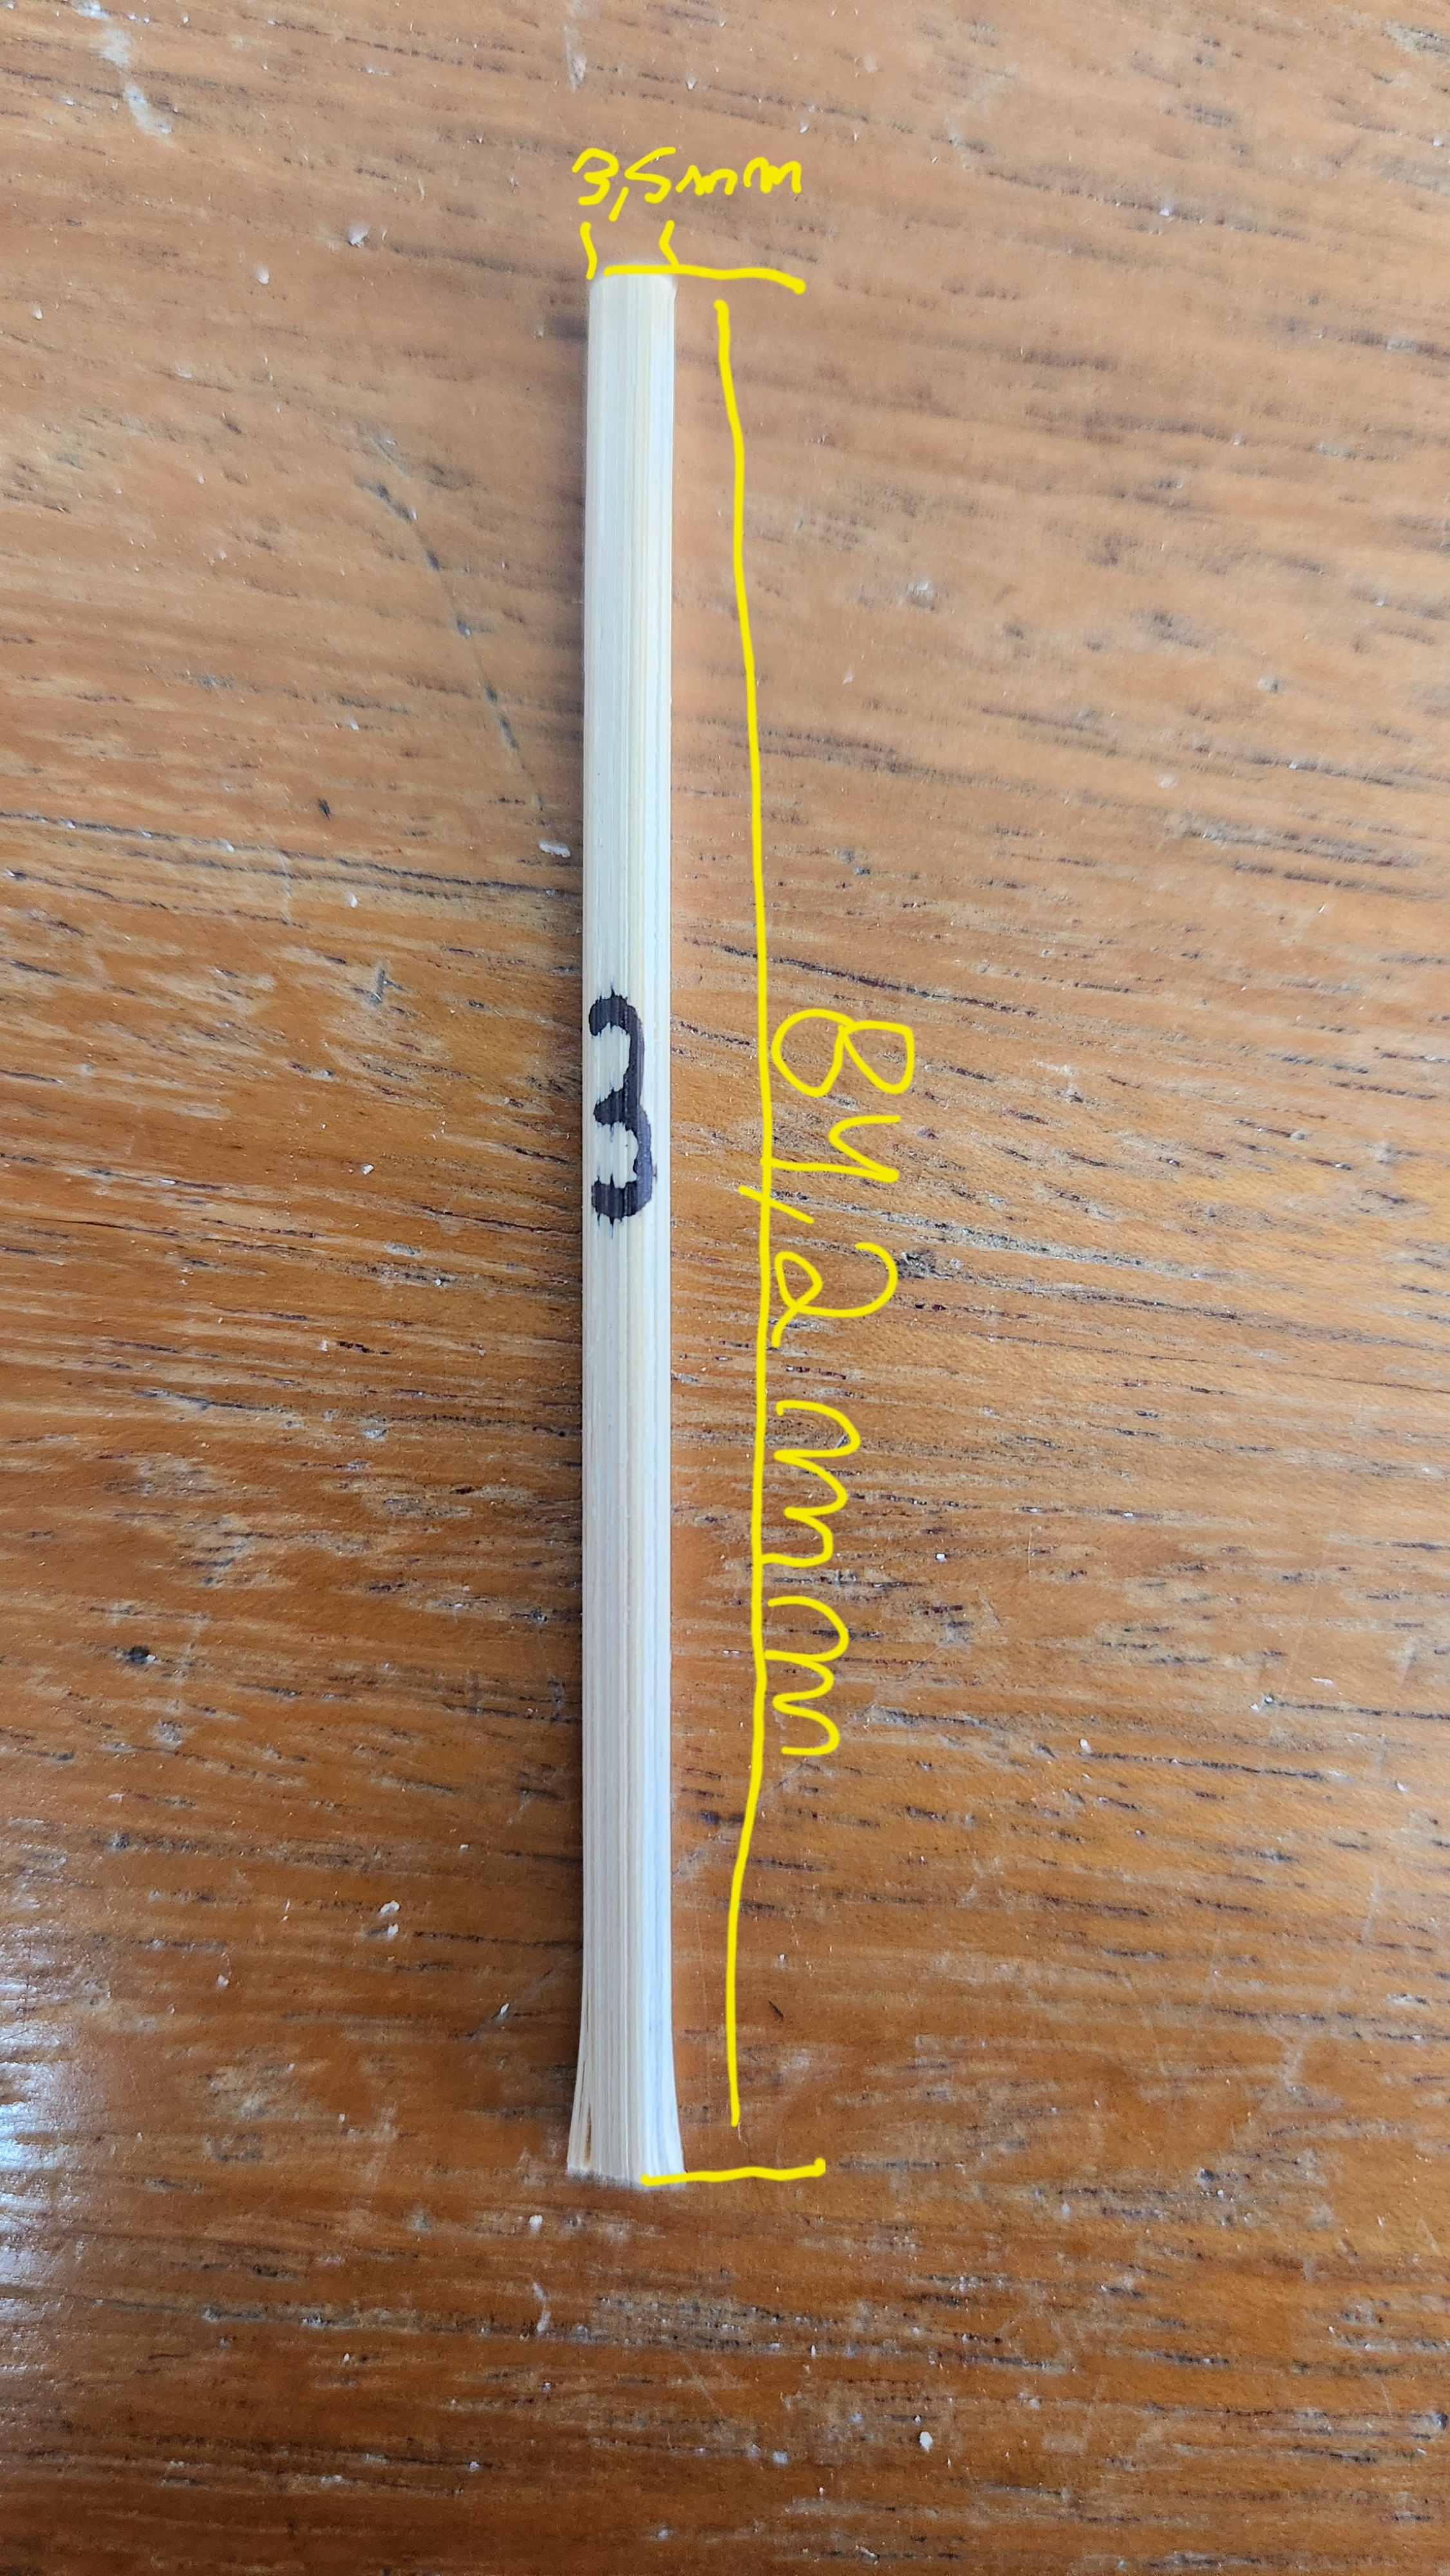
\includegraphics[width=10cm]{foto_parte3.jpg}
\caption{\label{fig:parte3}- Detalhe e dimensões do Quadril.}
\end{center}
\end{figure}

\begin{figure}[H]
\begin{center}
 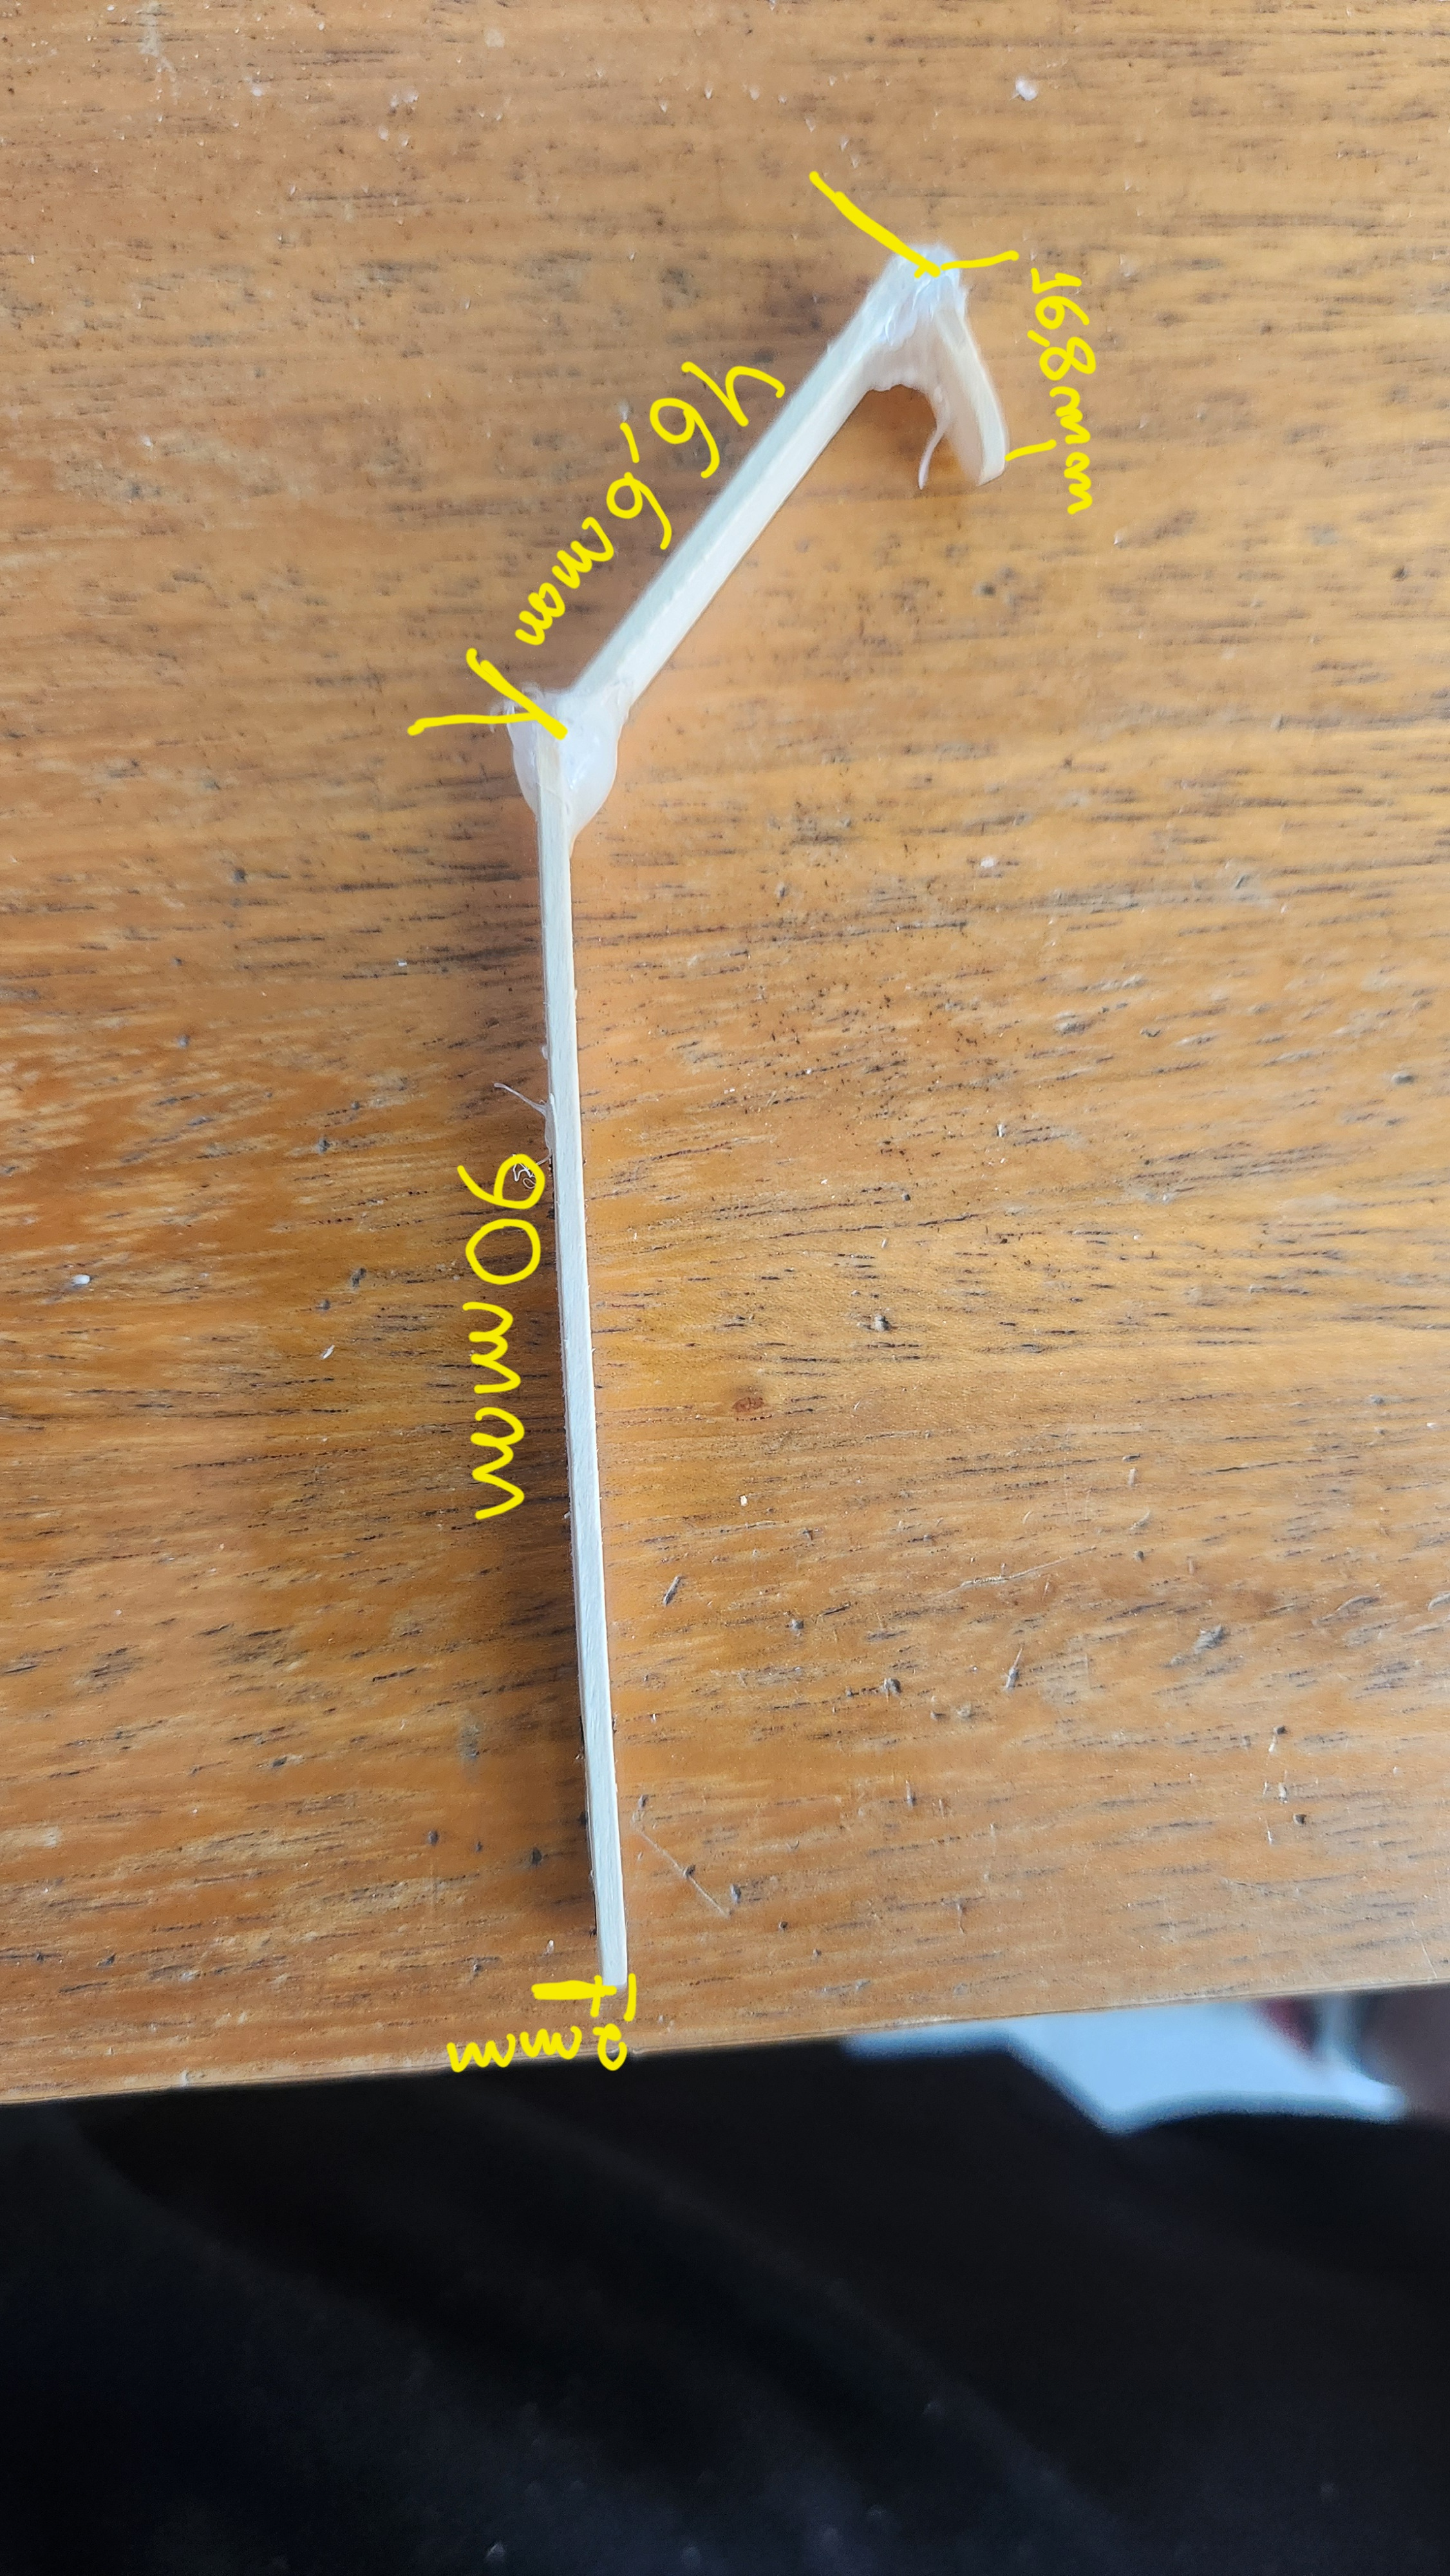
\includegraphics[width=10cm]{foto_parte4.jpg}
\caption{\label{fig:parte4}- Detalhe e dimensões do Braço.}
\end{center}
\end{figure}

\begin{figure}[H]
\begin{center}
 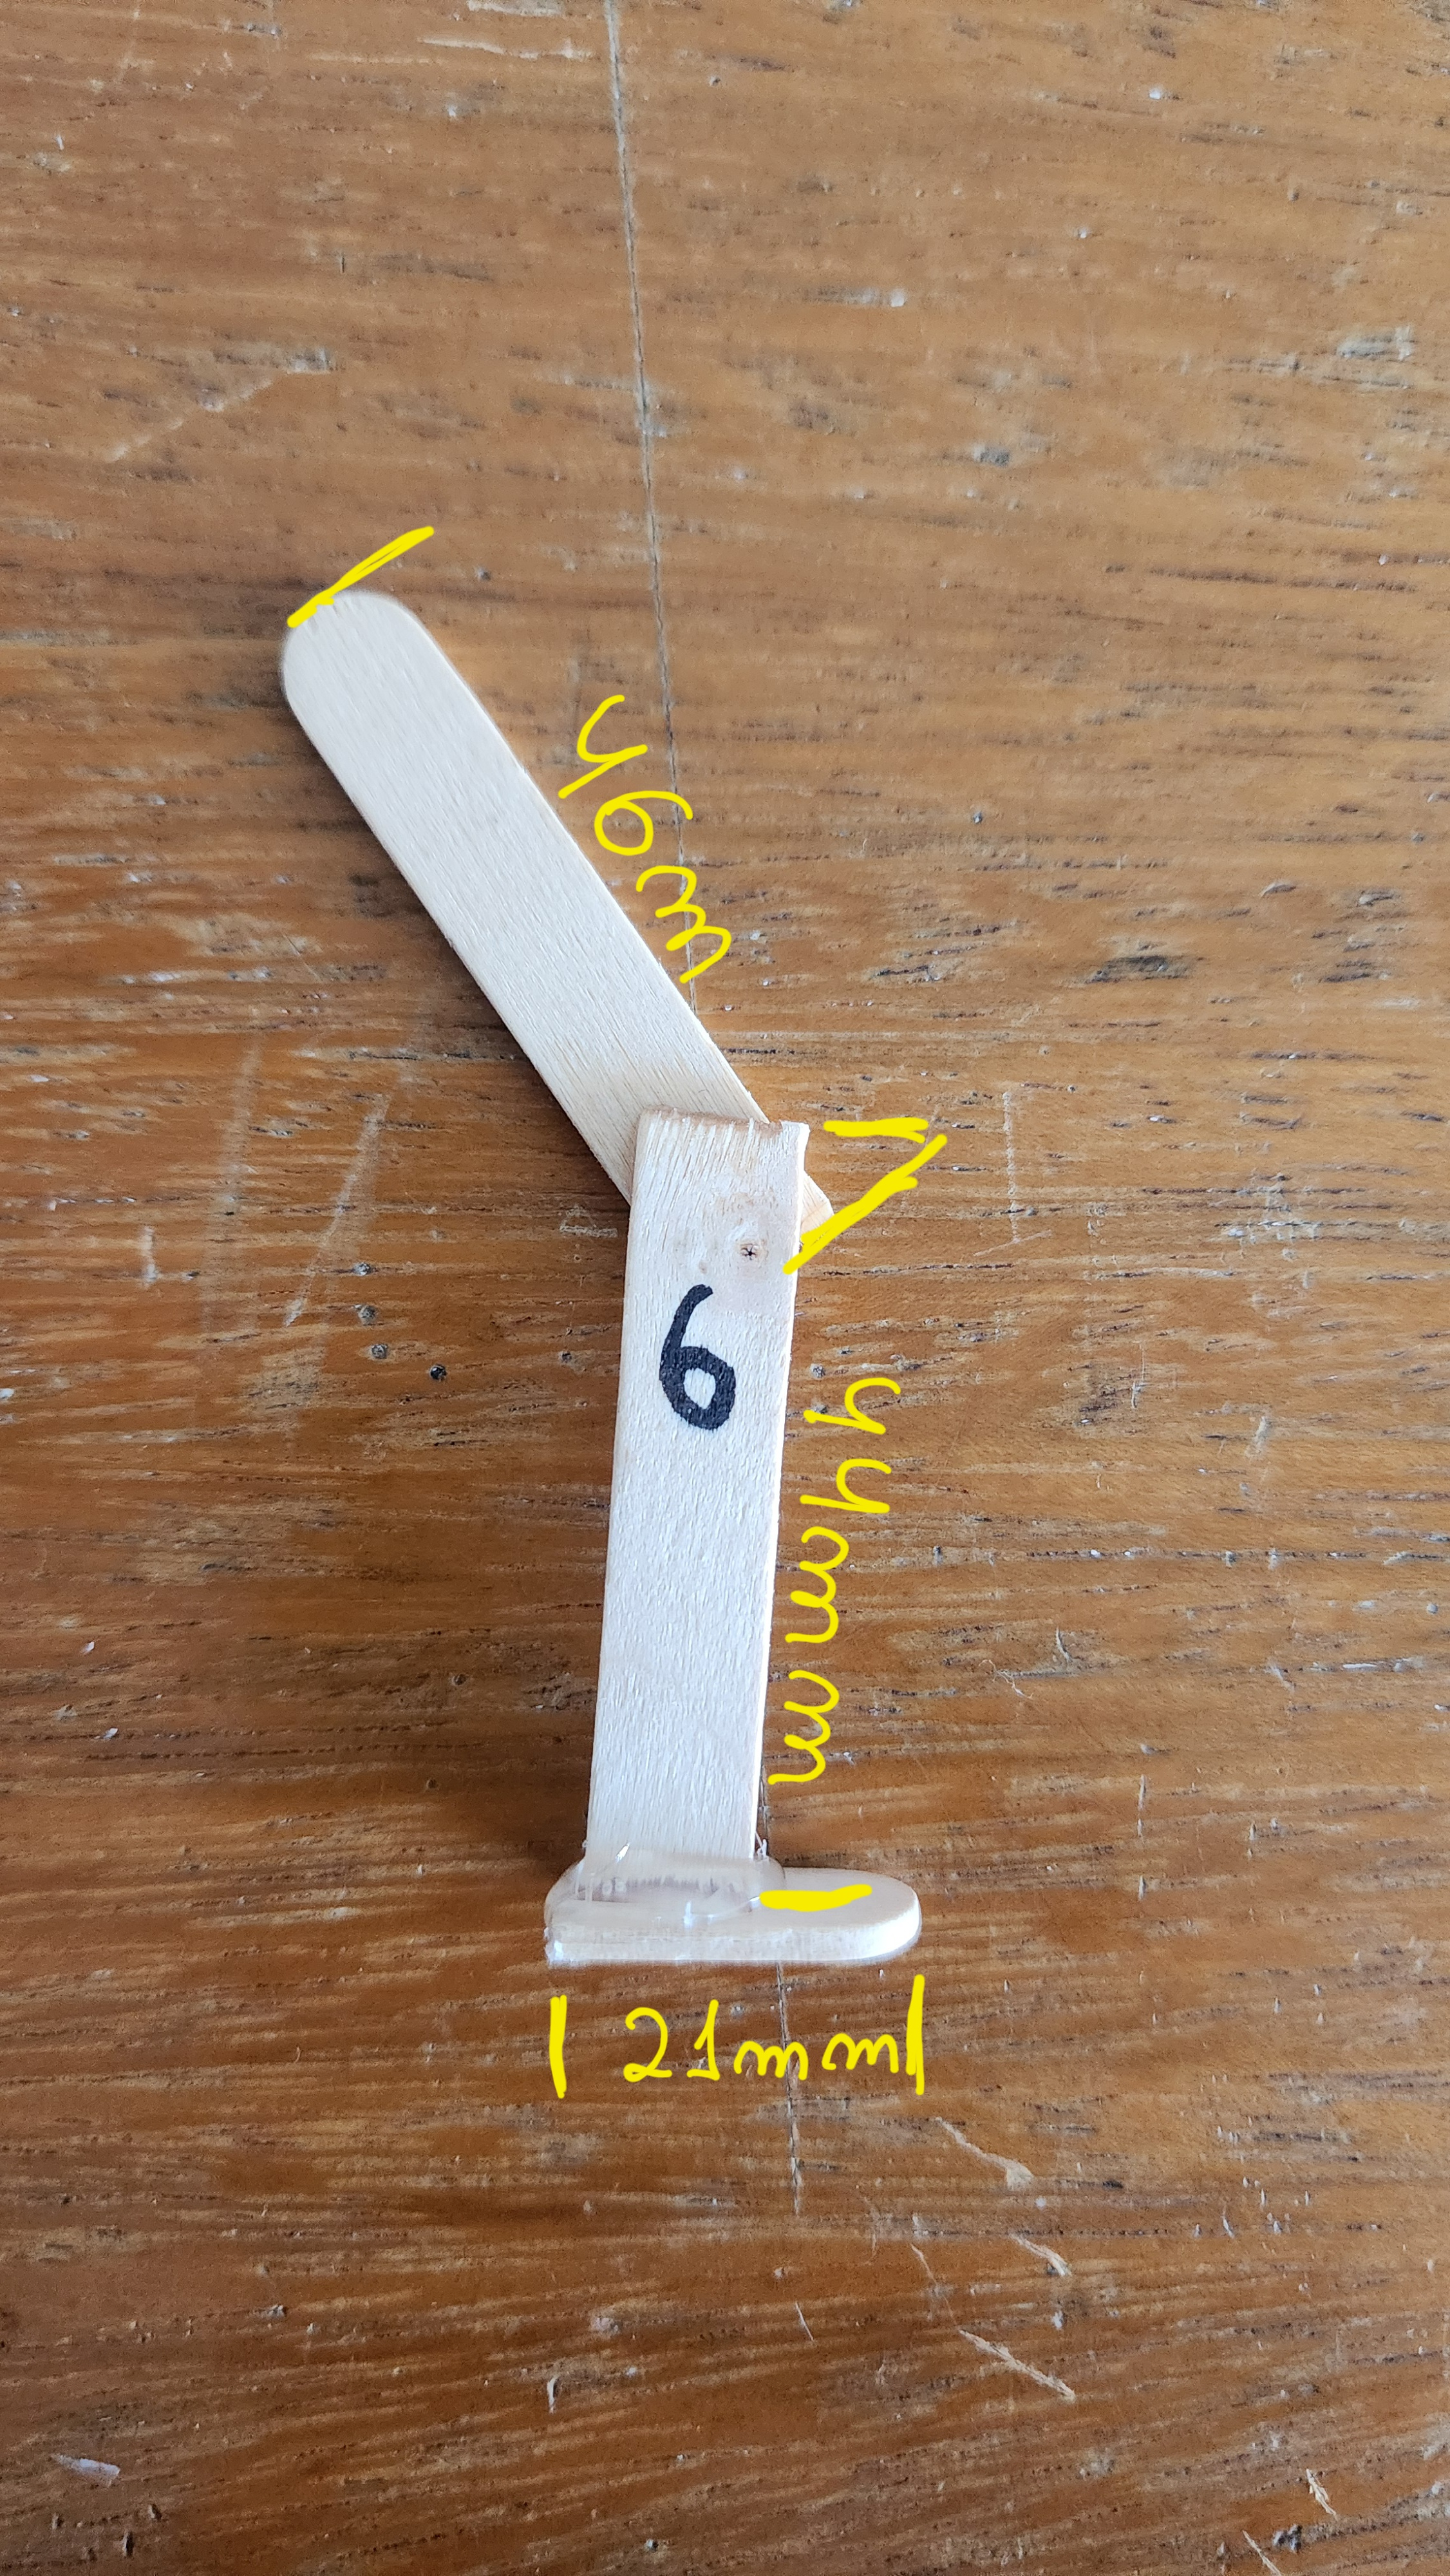
\includegraphics[width=10cm]{foto_parte5.jpg}
\caption{\label{fig:parte5}- Detalhe e dimensões da Perna (visão lateral).}
\end{center}
\end{figure}

\begin{figure}[H]
\begin{center}
 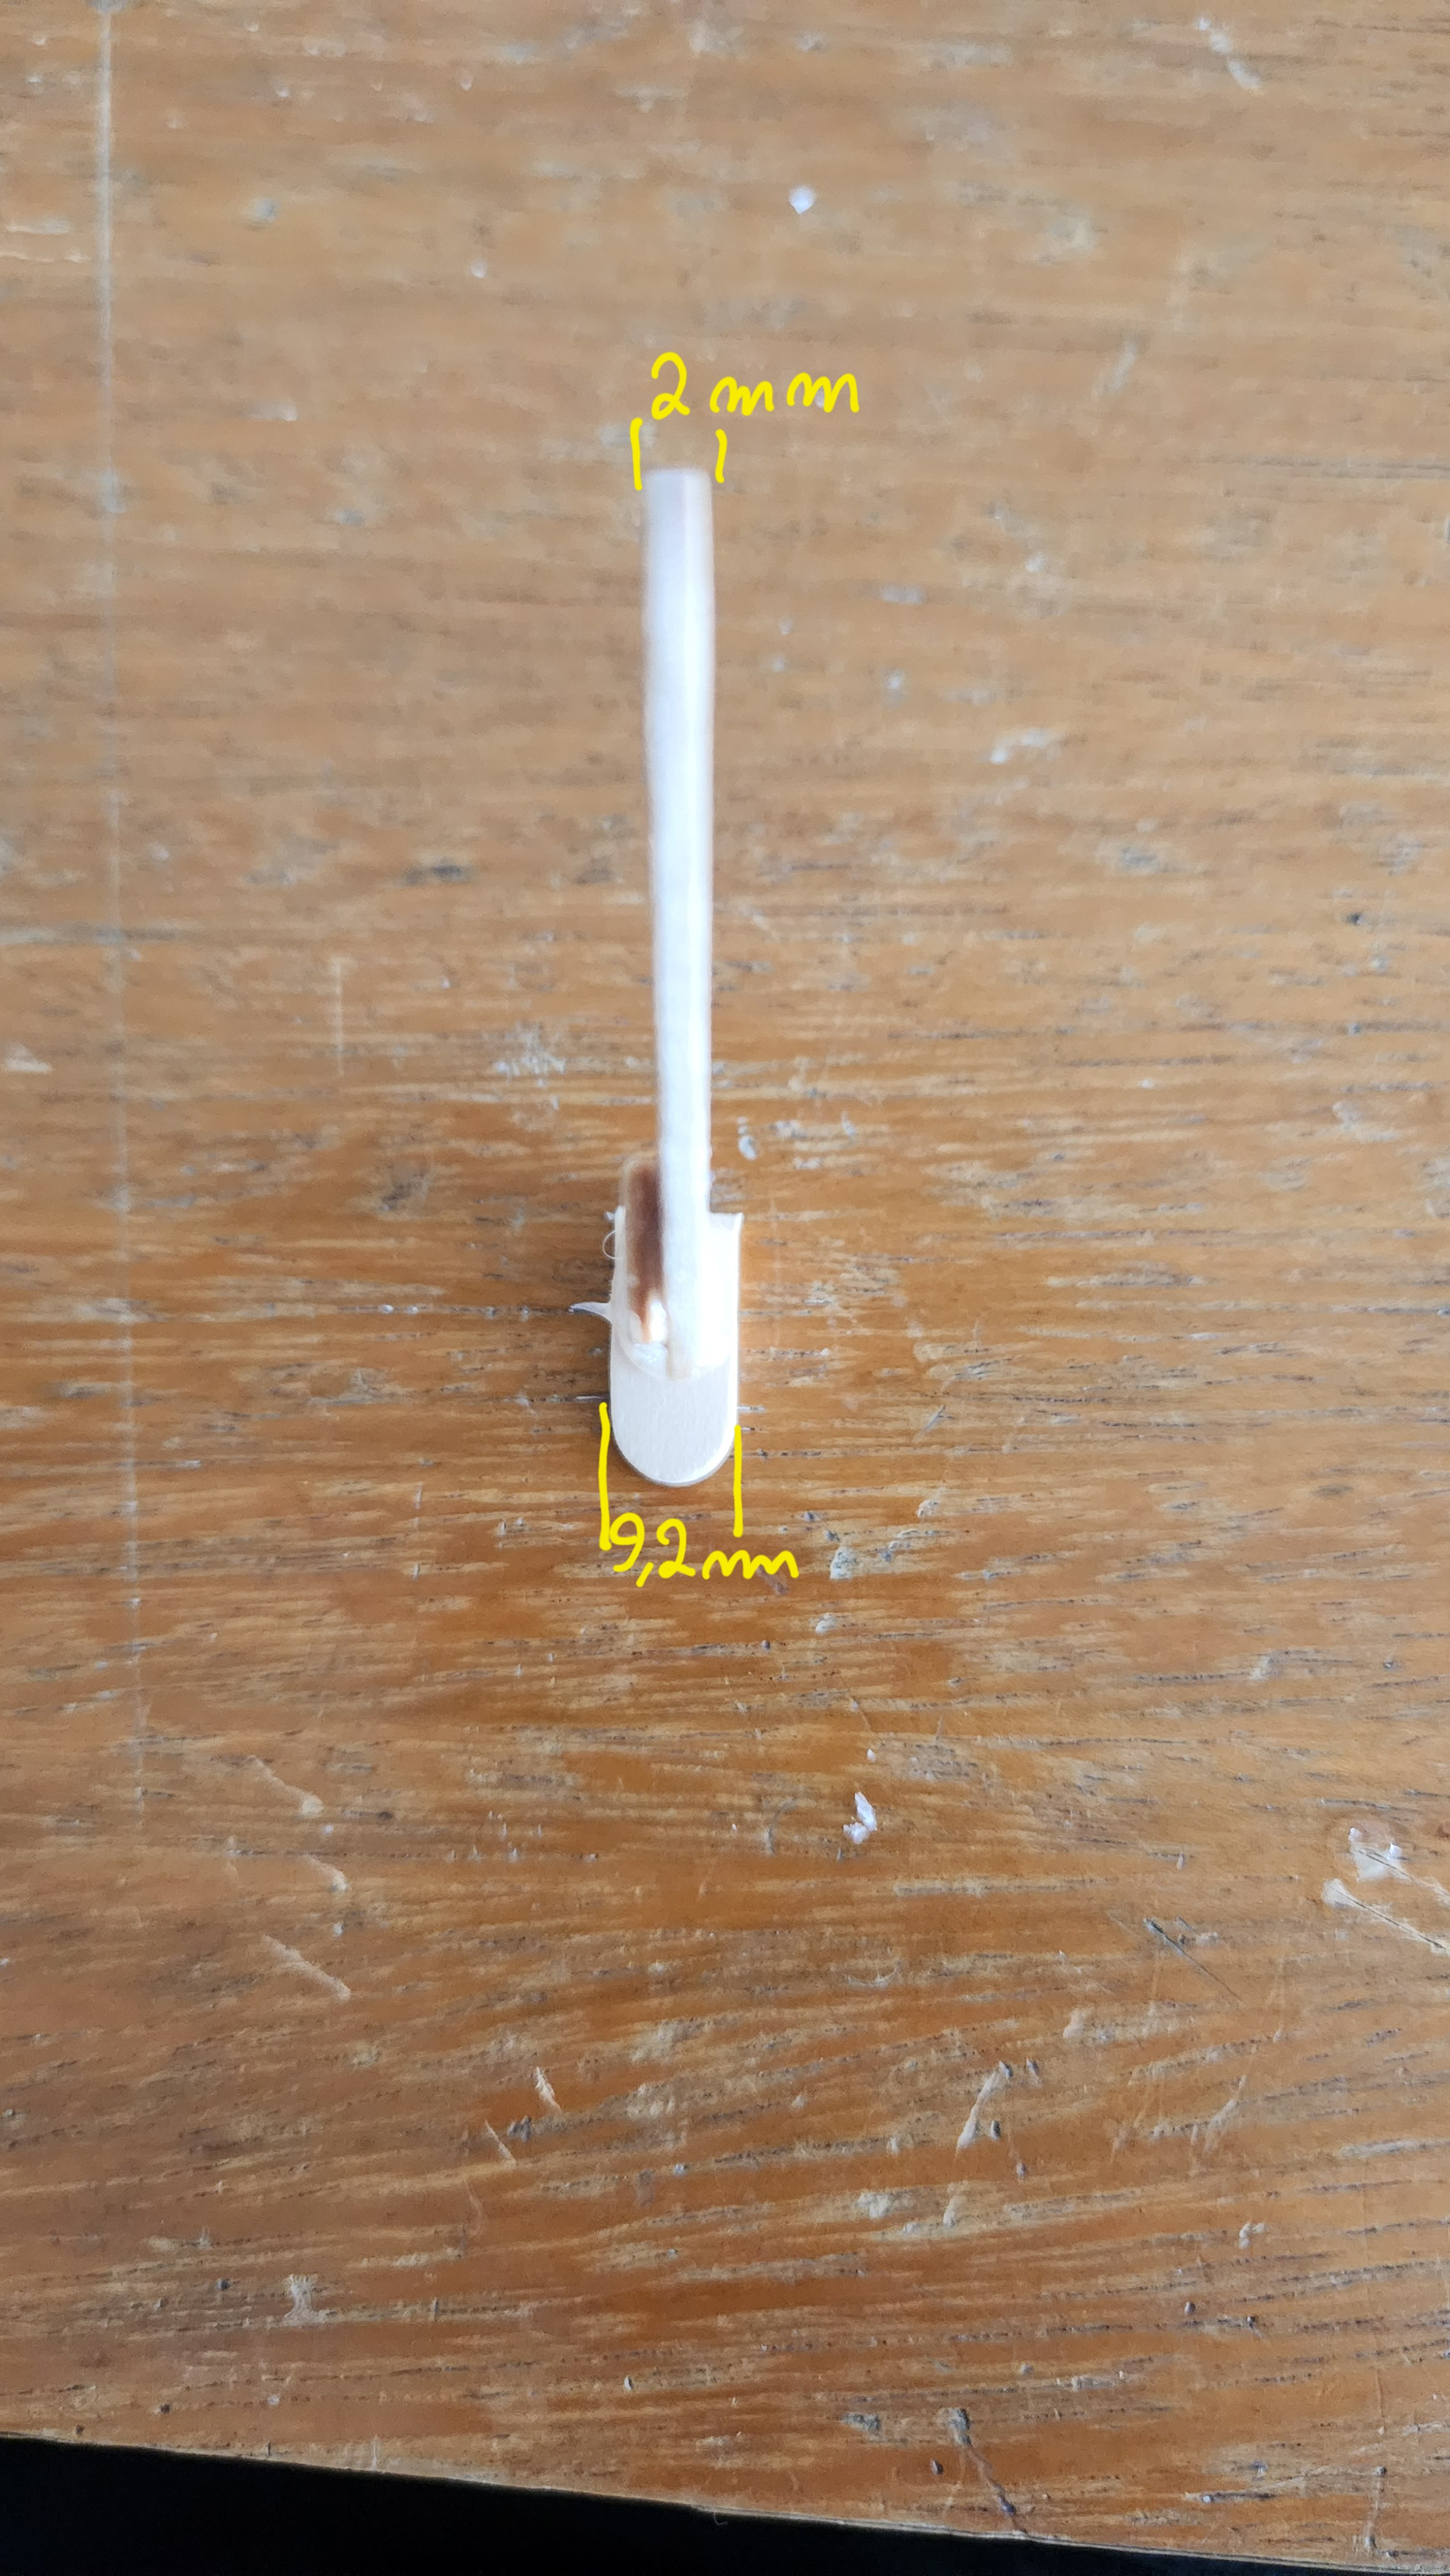
\includegraphics[width=10cm]{foto_parte6.jpg}
\caption{\label{fig:parte6}- Detalhe e dimensões da Perna (visão frontal).}
\end{center}
\end{figure}

\subsection{Medição dos Ângulos}

Os ângulos entre os segmentos do braço e da perna foram obtidos das fotografias das peças apoiadas sobre a bancada e fotografadas de cima. Em cada fotografia, os pixels de cada segmento foram isolados por um limiar de cor e de saturação, e uma reta foi ajustada a cada um por decomposição em valores singulares; o ângulo entre as direções das retas é o desvio entre os segmentos. Na perna, a junta entre as hastes resultou em um ângulo interno de 138,8$^\circ$. No braço, a medição com transferidor resultou em 130$^\circ$ e o ajuste de retas na fotografia da peça em 140,8$^\circ$ (desvio de 39,2$^\circ$); adotou-se o ângulo interno de 150$^\circ$, para o qual o avanço horizontal do segmento inclinado (23,3 mm) é praticamente igual à distância de 22 mm do plano do braço ao plano de simetria, de modo que as mãos se encontram sobre a corda, como se observa na vista frontal do protótipo. Na perna, as distâncias do calcanhar (7,0 mm) e do dedão (14,0 mm) ao eixo da haste foram obtidas da mesma fotografia, com o comprimento do pé (21 mm) como escala.

\subsection{Dimensões das Peças}

A \ref{tab:geometria} reúne as dimensões usadas no modelo. Todas as peças de madeira têm seção do palito de picolé (9,2 mm $\times$ 2,0 mm).

\begin{table}[H]
\centering
\caption{\label{tab:geometria}- Dimensões das peças utilizadas no modelo.}
\vspace*{.1cm}
\small
\begin{tabular}{|l|p{9.2cm}|}
\hline
\textbf{Peça} & \textbf{Dimensões} \\
\hline
Braço & segmentos de 90,0; 46,6 e 16,8 mm; ângulo interno da junta de 150$^\circ$ e do gancho de 70$^\circ$ \\
\hline
Perna & hastes de 44,0 e 46,0 mm; pé de 21,0 mm (calcanhar de 7,0 mm e dedão de 14,0 mm em relação ao eixo da haste); ângulo interno do joelho de 138,8$^\circ$ \\
\hline
Ombro & camada inferior de 19,2 mm e duas camadas de 13,0 mm, com 9,2 mm de largura e 5,5 mm de altura total; furo de 5,0 mm; pino de 3,5 mm de diâmetro e 29,1 mm de altura total; raio da manivela de 9,0 mm \\
\hline
Quadril & haste de 3,5 mm de diâmetro e 84,2 mm de comprimento \\
\hline
Motor com caixa de redução & caixa de 22,5 $\times$ 31,8 $\times$ 18,8 mm; comprimento total de 64,2 mm; corpo do motor de 15,0 $\times$ 30,0 $\times$ 22,5 mm (15,0 mm estimado); eixo duplo de 5,4 mm de diâmetro e 36,8 mm no total \\
\hline
Bateria & 33,55 $\times$ 13,9 $\times$ 67,7 mm \\
\hline
\end{tabular}
\end{table}

\subsection{Parâmetros Adotados}

Alguns parâmetros não foram medidos e foram adotados por hipótese; eles são listados na \ref{tab:adotados} e devem ser substituídos por valores medidos quando disponíveis.

\begin{table}[H]
\centering
\caption{\label{tab:adotados}- Parâmetros adotados por hipótese.}
\vspace*{.1cm}
\small
\begin{tabular}{|p{5.6cm}|p{4.2cm}|p{4.5cm}|}
\hline
\textbf{Parâmetro} & \textbf{Valor} & \textbf{Observação} \\
\hline
Repartição da massa do motor & 40\,\% na caixa e 60\,\% no motor & motor mais denso \\
\hline
Largura do corpo do motor & 15,0 mm & não consta do desenho \\
\hline
Massa dos palitos compostos & proporcional ao comprimento & seção e material iguais \\
\hline
Furo da perna no quadril & 4,6 mm da extremidade & metade da largura do palito \\
\hline
Posição da bateria & atrás da caixa, centrada & estimada da fotografia \\
\hline
Altura da junta do braço & 24 mm acima do eixo do motor & lida na fotografia frontal \\
\hline
Rotação do motor & 30 rpm no eixo de saída & valor suposto \\
\hline
Amortecimento & $c_{ch}=10^{-4}$ e $c_p=5\cdot10^{-5}$ N$\cdot$m$\cdot$s/rad & valores supostos \\
\hline
\end{tabular}
\end{table}

\chapter{TENSORES DE INÉRCIA DO PROTÓTIPO}
\label{chapter:inercia}

Este capítulo apresenta o cálculo da massa, do centro de massa e do tensor de inércia de cada peça do robô e do conjunto montado. Todos os cálculos seguem o procedimento da Seção \ref{sec:composicao}: cada peça é decomposta em sólidos homogêneos elementares (paralelepípedos e cilindros), cujos tensores no centro de massa são conhecidos (Equações \ref{eq:Ipar} e \ref{eq:Icil}); esses tensores são girados para o sistema da peça e transportados para o centro de massa do conjunto pelo teorema dos eixos paralelos (Equação \ref{eq:steiner}). Os cálculos foram implementados em Python com a biblioteca SymPy, e as massas parciais das peças de madeira foram distribuídas proporcionalmente ao volume (ou, para barras de mesma seção, ao comprimento), supondo densidade uniforme. Os valores de tensor estão expressos em g$\cdot$mm$^2$ (1 g$\cdot$mm$^2 = 10^{-9}$ kg$\cdot$m$^2$) e as posições em mm.

\section{Convenções de Eixos}
\label{sec:eixos}

Cada peça é descrita em um sistema próprio, com o plano $x$--$y$ coincidindo com o plano da dobra (no caso de braço e perna) e o eixo $z$ perpendicular a ele. No robô montado adota-se o sistema do corpo: origem $O$ no centro do eixo de saída do motor, eixo $z$ ao longo desse eixo (da esquerda para a direita na vista frontal), eixo $y$ para cima e eixo $x$ para o fundo, de modo que $+x$ aponta para as costas do robô e $-x$ para a frente (lado do rosto). Os lados direito (D) e esquerdo (E) correspondem a $z>0$ e $z<0$.

\section{Resultados por Peça}
\label{sec:resultados_pecas}

\subsection{Braço}

O braço é composto por três barras finas (\ref{fig:braco_modelo}): o segmento longo (90,0 mm), o segmento inclinado (46,6 mm) e o gancho (16,8 mm), todos com seção de 9,2 mm $\times$ 2,0 mm e massa total de 2,00 g, distribuída proporcionalmente ao comprimento (1,17 g, 0,61 g e 0,22 g). O ângulo interno entre o segmento longo e o inclinado vale 150$^\circ$ (desvio de 30$^\circ$) e o ângulo interno do gancho vale 70$^\circ$. A origem do sistema da peça é a extremidade livre do segmento longo, com $y$ ao longo dele. Os resultados são:

\begin{figure}[H]
\begin{center}
 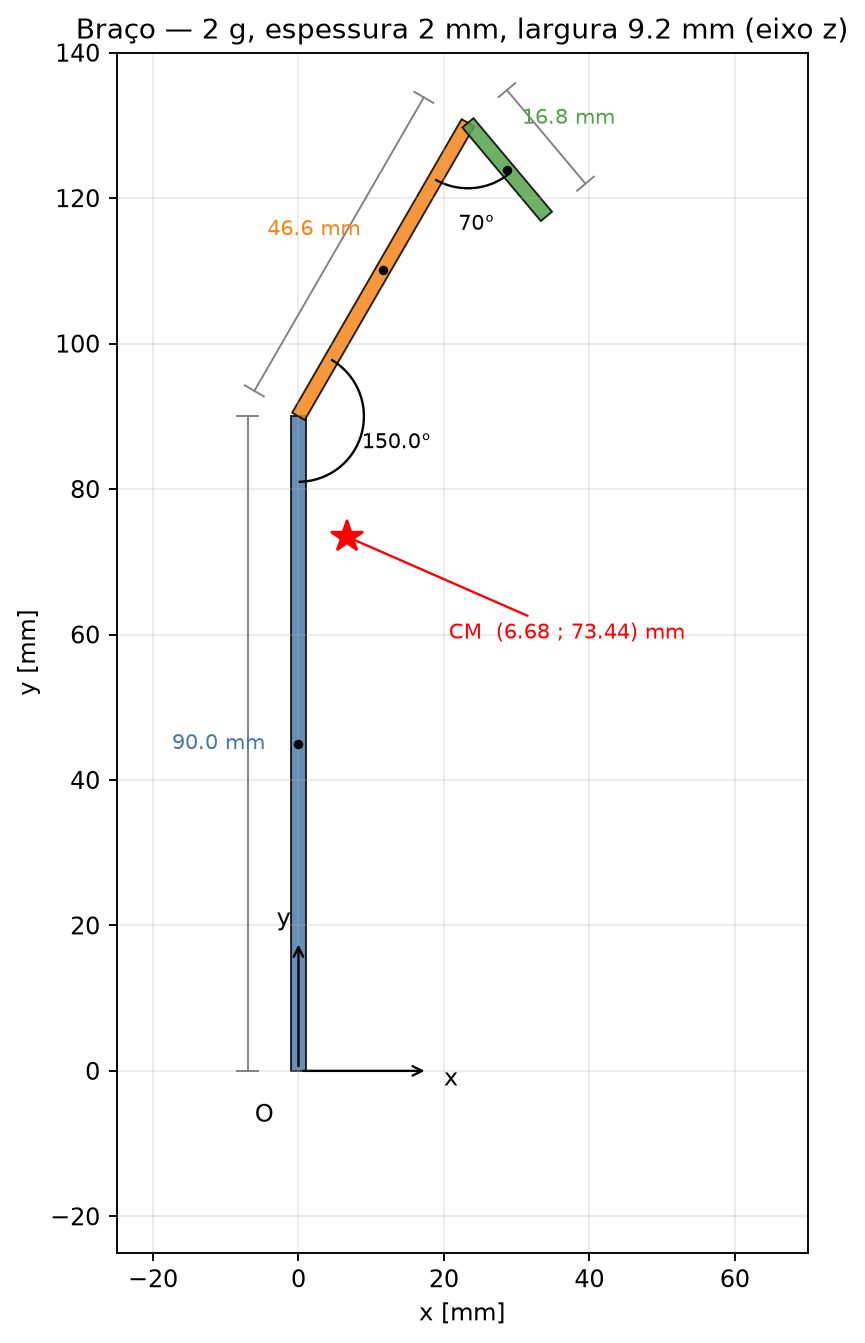
\includegraphics[height=9.5cm]{braco.png}
\caption{\label{fig:braco_modelo}- Modelo do braço (escala real), com cotas, ângulos internos e centro de massa (estrela).}
\end{center}
\end{figure}

\begin{equation*}
\vec{r}_{cm} = (6{,}68; 73{,}44; 0)\ \text{mm}, \qquad [I^*_{\text{braço}}] = \begin{bmatrix}3219{,}0 & -622{,}4 & 0 \\
-622{,}4 & 217{,}9 & 0 \\
0 & 0 & 3408{,}7
\end{bmatrix}\ \text{g}\cdot\text{mm}^2,
\end{equation*}

\noindent com momentos principais de 93,9; 3343,0; 3408,7 g$\cdot$mm$^2$. O produto de inércia $I_{xy}$ não nulo decorre da dobra do braço, e a nulidade de $I_{xz}$ e $I_{yz}$ confirma que o plano da dobra é um plano de simetria de massa.

\subsection{Perna}

A perna é formada por três barras (\ref{fig:perna_modelo}): a haste inferior (44,0 mm), a haste superior inclinada (46,0 mm) e o pé (21,0 mm), com massa total de 1,50 g repartida proporcionalmente ao comprimento (0,59 g, 0,62 g e 0,28 g). O ângulo interno do joelho, medido na fotografia da perna, vale 138,8$^\circ$. O pé não é centrado na haste: a partir do eixo da haste, o calcanhar mede 7,0 mm e o dedão 14,0 mm, de modo que o centro do pé fica deslocado 3,5 mm para a frente. A origem é a extremidade inferior da haste de 44 mm.

\begin{figure}[H]
\begin{center}
 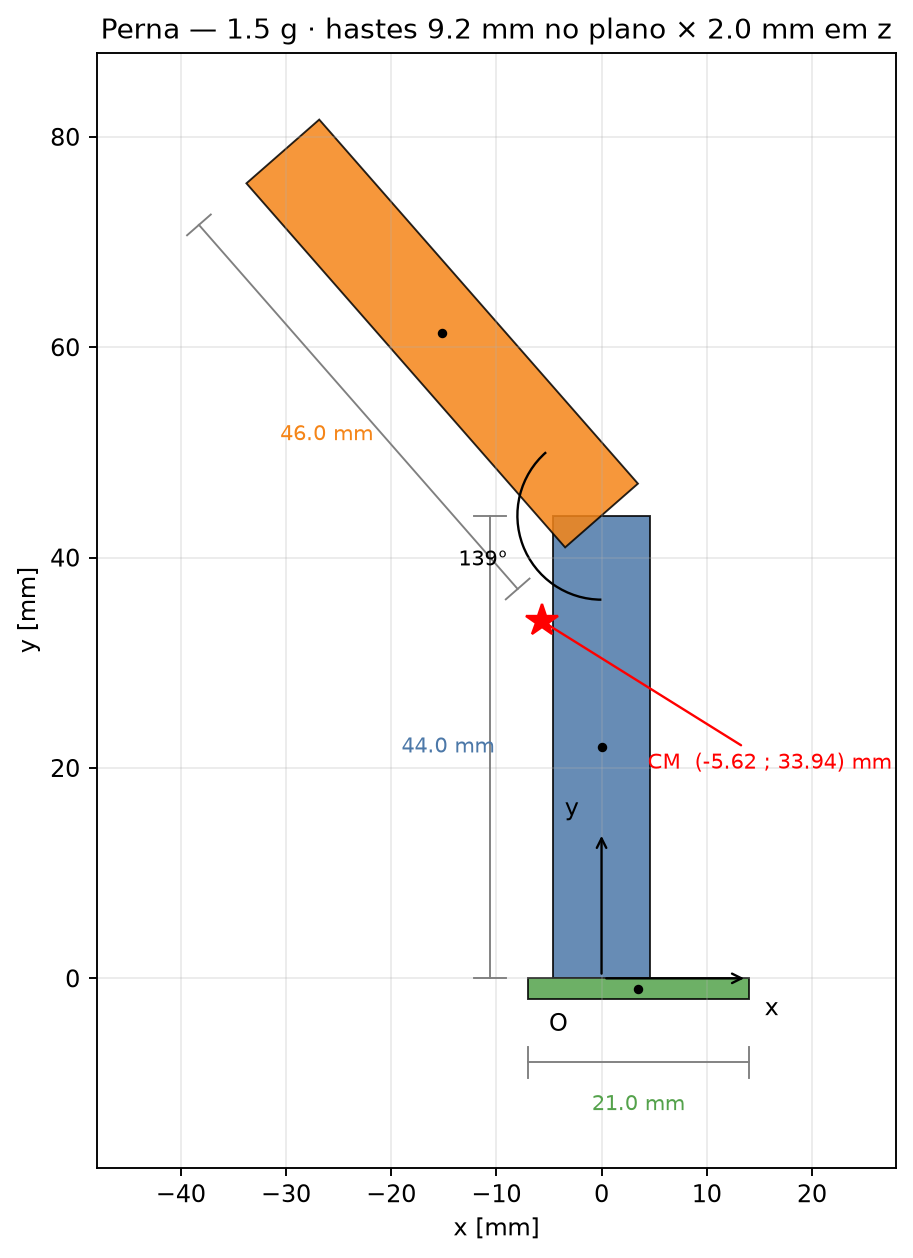
\includegraphics[height=9.5cm]{perna.png}
\caption{\label{fig:perna_modelo}- Modelo da perna (escala real), com calcanhar e dedão.}
\end{center}
\end{figure}

\begin{equation*}
\vec{r}_{cm} = (-5{,}62; 33{,}94; 0)\ \text{mm}, \qquad [I^*_{perna}] = \begin{bmatrix}1059{,}1 & 344{,}6 & 0 \\
344{,}6 & 165{,}9 & 0 \\
0 & 0 & 1220{,}2
\end{bmatrix}\ \text{g}\cdot\text{mm}^2,
\end{equation*}

\noindent com momentos principais de 48,4; 1176,6; 1220,2 g$\cdot$mm$^2$.

\subsection{Ombro (manivela)}

O ombro é a peça que acopla o eixo do motor às alavancas. É formado por uma pilha de três camadas de palito (a inferior com 19,2 mm de comprimento e as duas superiores com 13,0 mm, todas com 9,2 mm de largura e 5,5 mm de altura total), um furo passante de 5,0 mm de diâmetro para o eixo do motor e um pino de 3,5 mm de diâmetro apoiado na camada inferior, cujo eixo dista 9,0 mm do eixo do furo (raio da manivela) e cuja extremidade livre fica a 29,1 mm da face inferior da pilha (\ref{fig:ombro_modelo}). O furo foi tratado como massa negativa, e a massa total de 0,83 g foi distribuída pelo volume. O sistema da peça tem origem no eixo do furo, na face inferior da base, com $z$ ao longo do eixo.

\begin{figure}[H]
\begin{center}
 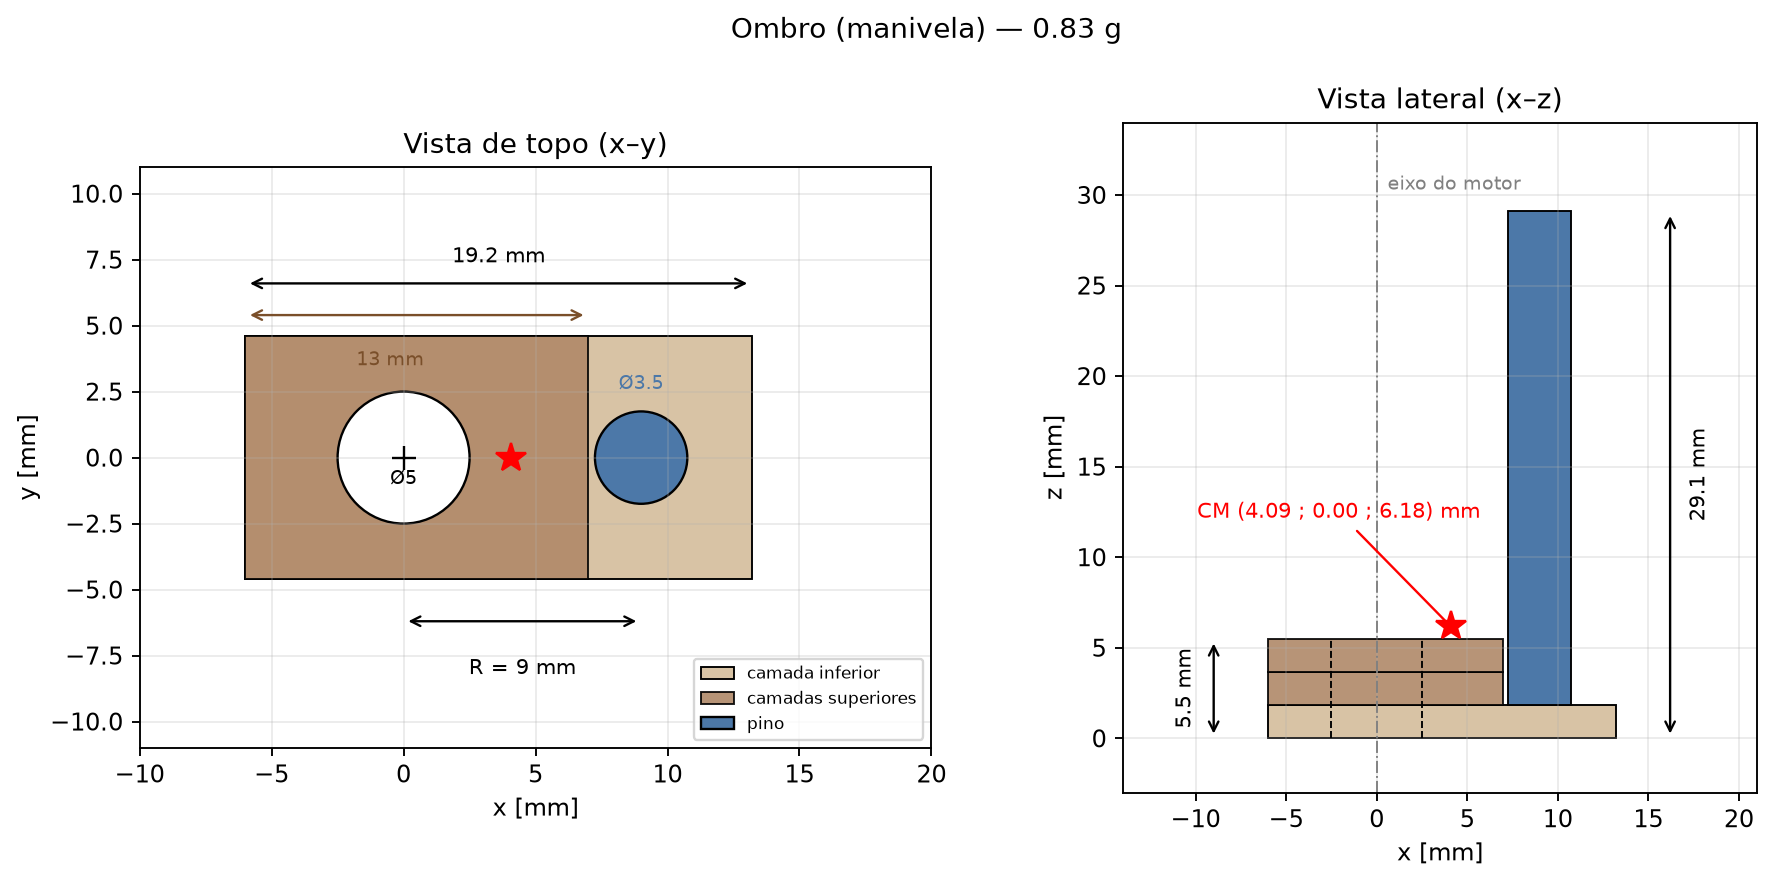
\includegraphics[width=14cm]{ombro.png}
\caption{\label{fig:ombro_modelo}- Modelo do ombro: vistas de topo e lateral, com furo, pino e centro de massa.}
\end{center}
\end{figure}

\begin{equation*}
\vec{r}_{cm} = (4{,}09; 0; 6{,}18)\ \text{mm}, \qquad [I^*_{ombro}] = \begin{bmatrix}49{,}9 & 0 & -13{,}8 \\
0 & 68{,}9 & 0 \\
-13{,}8 & 0 & 28{,}8
\end{bmatrix}\ \text{g}\cdot\text{mm}^2.
\end{equation*}

\noindent O momento de inércia em torno do eixo do motor, obtido por $I_{zz}^* + m\,d^2$, vale $J_{eixo} = 42,7$ g$\cdot$mm$^2$ ($4{,}27\cdot 10^{-8}$ kg$\cdot$m$^2$). O centro de massa fica a 4,1 mm do eixo, o que torna a manivela também uma massa excêntrica.

\subsection{Motor com caixa de redução}

O motor é do tipo com caixa de redução plástica, cujas dimensões foram obtidas do desenho técnico do fabricante (\ref{fig:desenho_motor}): caixa de 22,5 mm $\times$ 31,8 mm $\times$ 18,8 mm, eixo de saída duplo de 5,4 mm de diâmetro (salientes de 8,5 mm e 9,5 mm, totalizando 36,8 mm), comprimento total de 64,2 mm e centro do eixo a 11,2 mm do topo da caixa. O corpo do motor tem 30,0 mm de comprimento e 22,5 mm ao longo do eixo; sua dimensão na outra direção (15,0 mm) não consta do desenho e foi estimada. A massa do conjunto foi medida em 26,6 g, sendo 40\,\% atribuídos à caixa de redução e aos eixos e 60\,\% ao motor, que é mais denso por conter ímãs, bobinas e carcaça metálica. O sistema da peça tem origem no centro do eixo de saída, com $y$ apontando do motor para a caixa. A Figura \ref{fig:motor_modelo} apresenta o modelo sólido do conjunto nas vistas frontal e lateral.

\begin{figure}[H]
\begin{center}
 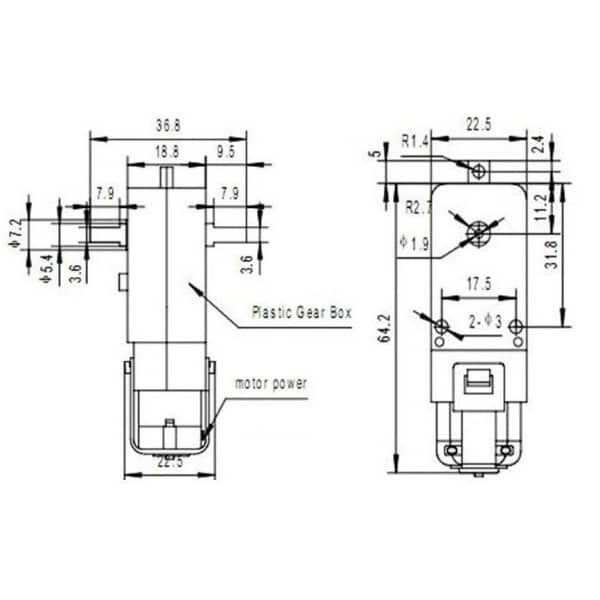
\includegraphics[width=7.5cm]{foto_desenho_motor_dc.jpg}
\caption{\label{fig:desenho_motor}- Desenho técnico do motor com caixa de redução (cotas em mm).}
\end{center}
\end{figure}

\begin{figure}[H]
\begin{center}
 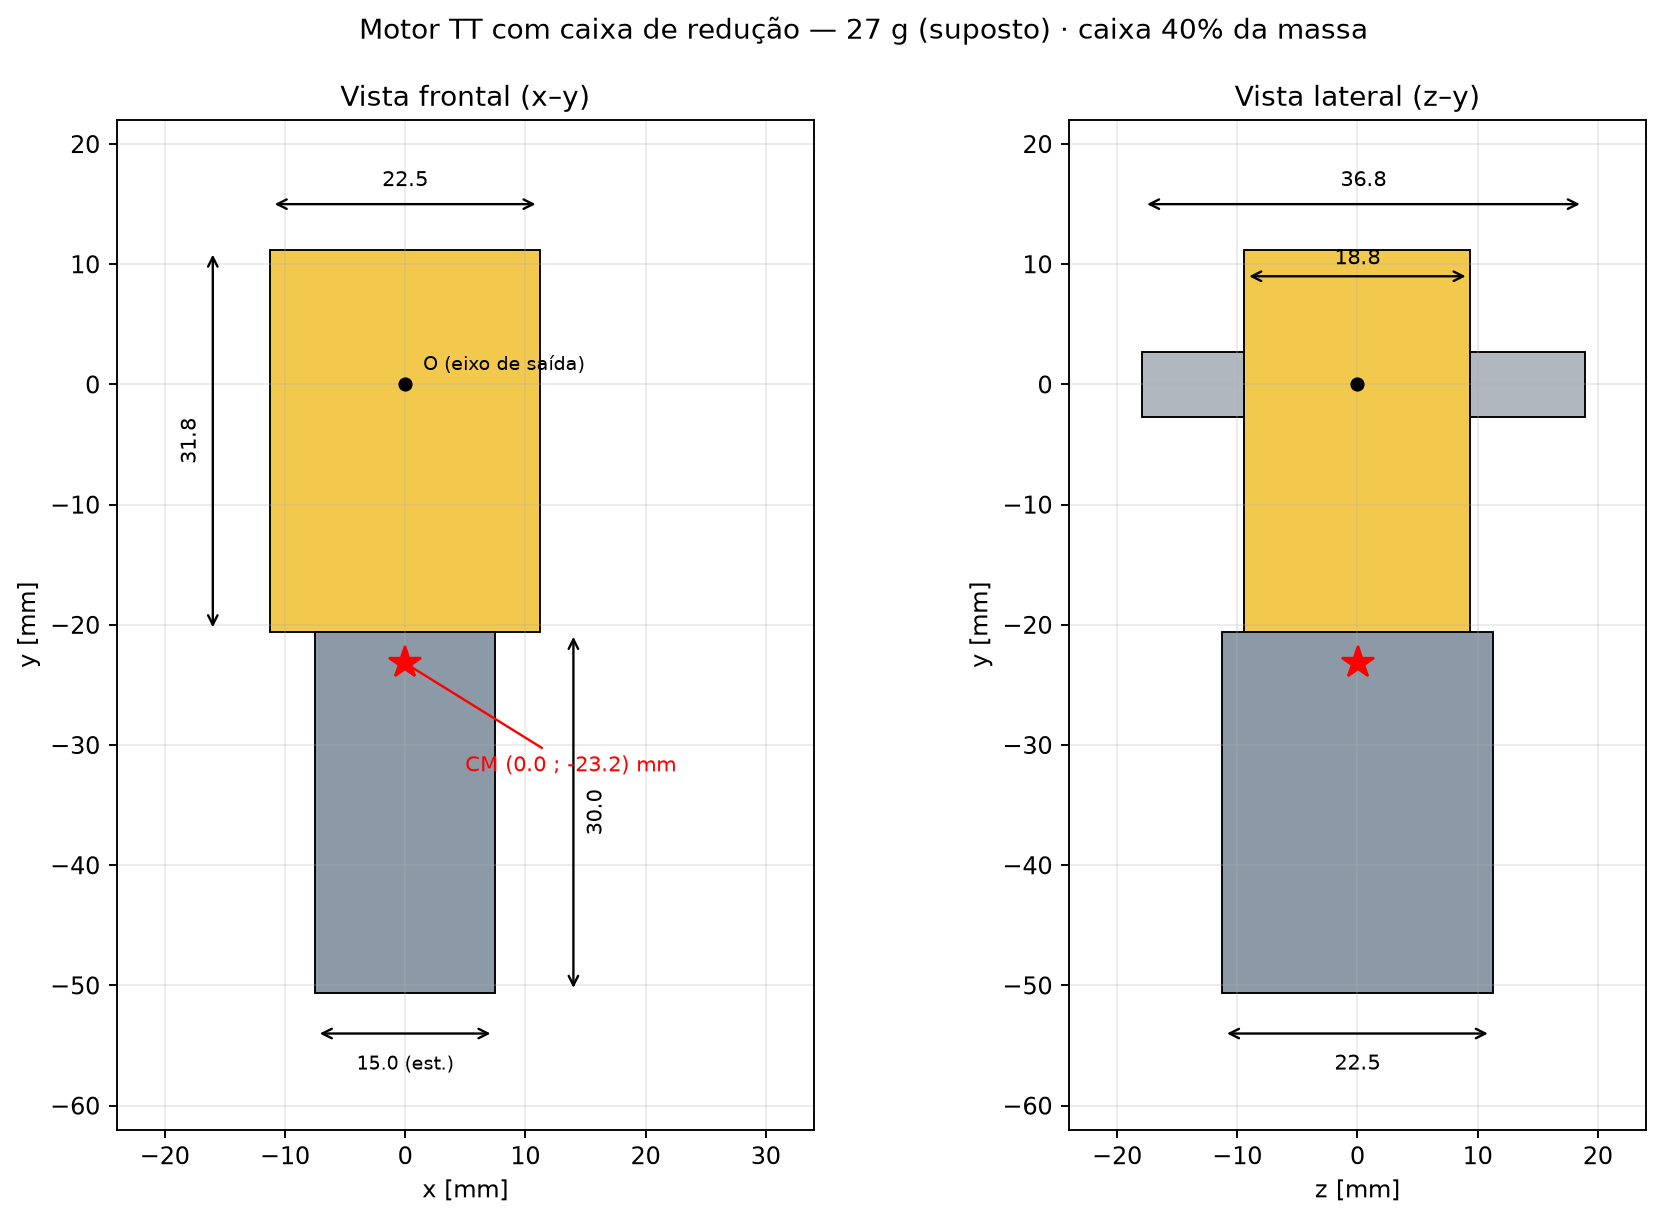
\includegraphics[width=13cm]{motor.png}
\caption{\label{fig:motor_modelo}- Modelo do motor (vistas frontal e lateral).}
\end{center}
\end{figure}

\begin{equation*}
\vec{r}_{cm} = (0; -23{,}18; 0{,}01)\ \text{mm}, \qquad [I^*_{motor}] = \begin{bmatrix}9265{,}9 & 0 & 0 \\
0 & 1776{,}2 & -7{,}5 \\
0 & -7{,}5 & 8960{,}5
\end{bmatrix}\ \text{g}\cdot\text{mm}^2.
\end{equation*}

\subsection{Bateria}

A bateria é um paralelepípedo de 33,55 mm $\times$ 13,9 mm $\times$ 67,7 mm e massa de 67,0 g, o que corresponde a uma densidade média de 2,12 g/cm$^3$, valor coerente com o de uma bateria de lítio. Tratada como sólido homogêneo, seu tensor no centro de massa é diagonal (\ref{fig:bateria_modelo}):

\begin{equation*}
[I^*_{bateria}] = \begin{bmatrix}26680{,}7 & 0 & 0 \\
0 & 31888{,}9 & 0 \\
0 & 0 & 7366{,}7
\end{bmatrix}\ \text{g}\cdot\text{mm}^2.
\end{equation*}

\begin{figure}[H]
\begin{center}
 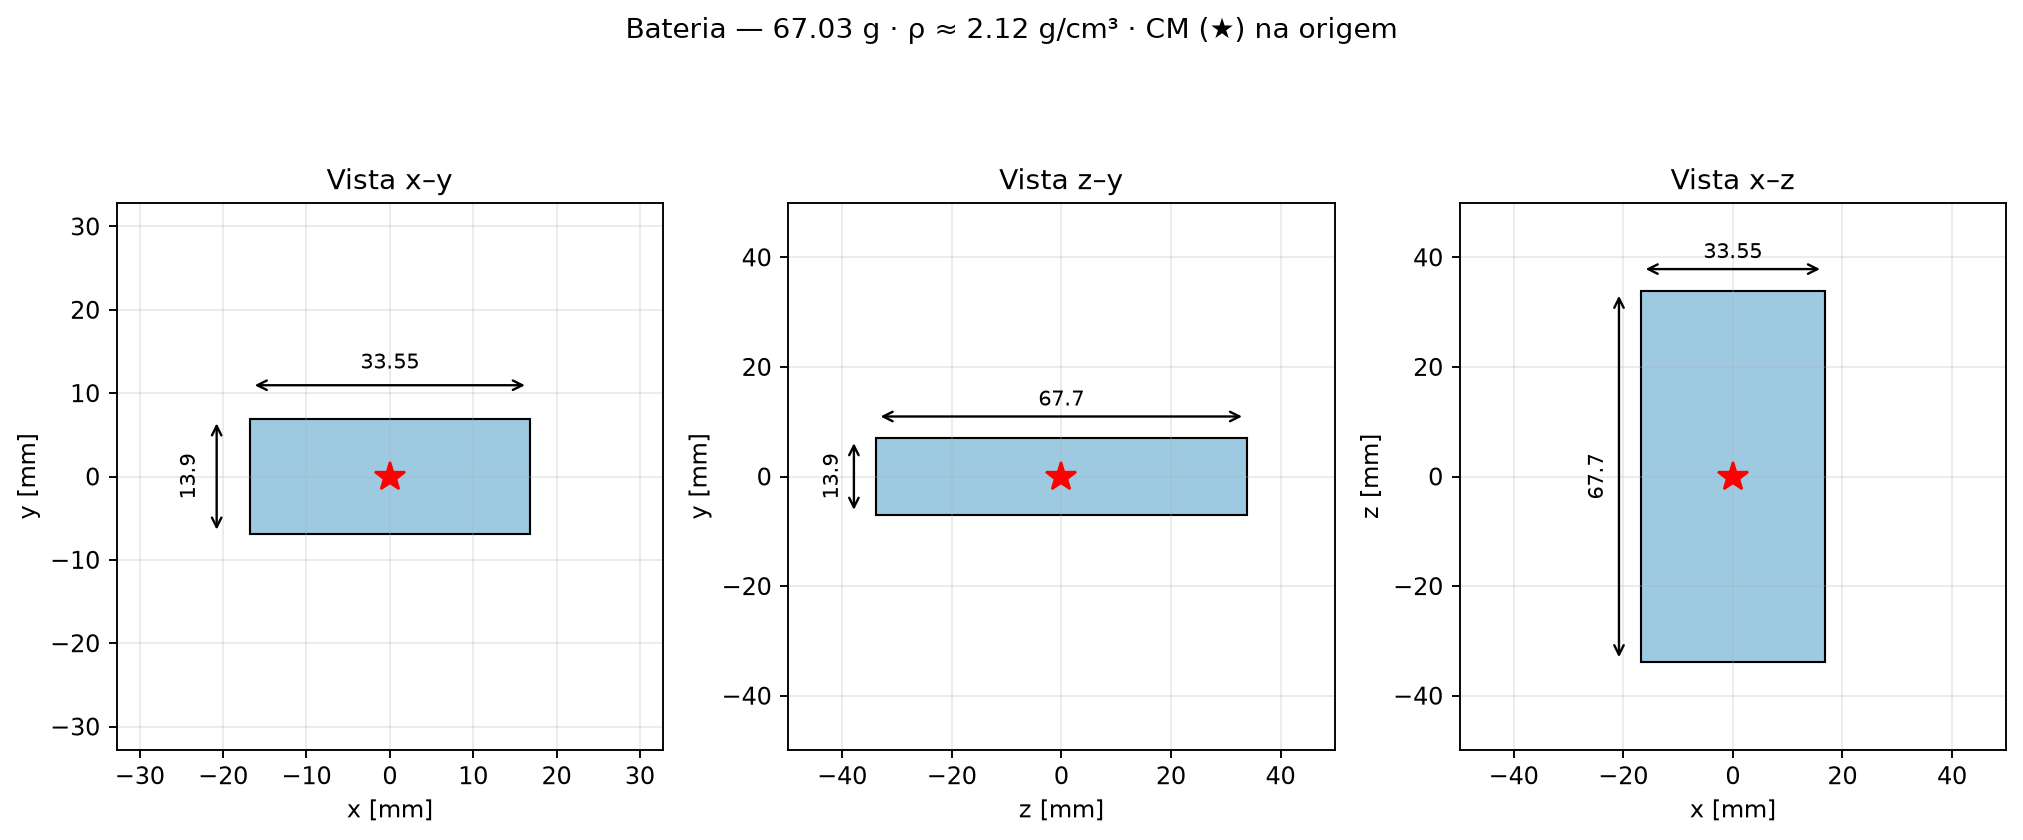
\includegraphics[width=14cm]{bateria.png}
\caption{\label{fig:bateria_modelo}- Modelo da bateria, em três vistas.}
\end{center}
\end{figure}

\subsection{Quadril}

O quadril é uma haste cilíndrica de 3,5 mm de diâmetro e 84,2 mm de comprimento, com massa de 0,81 g. Sua densidade seria de 1,00 g/cm$^3$ se a seção fosse circular e de 0,79 g/cm$^3$ se fosse quadrada, mas a diferença entre as duas hipóteses no momento de inércia transversal é de apenas 0,04\,\%. Com o eixo ao longo de $z$:

\begin{equation*}
[I^*_{quadril}] = \begin{bmatrix}479{,}2 & 0 & 0 \\
0 & 479{,}2 & 0 \\
0 & 0 & 1{,}2
\end{bmatrix}\ \text{g}\cdot\text{mm}^2,
\end{equation*}

\noindent ou seja, a haste comporta-se como uma barra fina ($I \approx mL^2/12$ nas direções transversais).

\section{Montagem do Robô Completo}
\label{sec:montagem}

A posição relativa das peças foi definida a partir da vista frontal do protótipo (\ref{fig:frontal}), que fornece duas cotas: 42 mm entre os palitos dos dois membros e 45,5 mm entre o eixo do motor (nível dos pinos das manivelas) e o eixo do quadril. Adotou-se:

\begin{itemize}
  \item membros nos planos $z=\pm 22$ mm (folga de 42 mm mais 2 mm de espessura) e quadril em $y=-45{,}5$ mm;
  \item manivelas montadas nos dois lados da caixa, com os pinos defasados de 180$^\circ$, de modo que, quando um braço vai para trás, o outro vai para a frente;
  \item braços como corpos rígidos que giram em torno do eixo do quadril e passam pelos pinos das manivelas (Seção \ref{sec:alavancas}), com extremidade inferior livre em $y=-66$ mm;
  \item pernas penduradas do eixo do quadril, com o furo do quadril 4,6 mm abaixo da extremidade superior da perna (estimado), dedão voltado para a frente e calcanhar atrás;
  \item bateria nas costas do robô, encostada na face traseira da caixa de redução e centrada em relação ao conjunto motor--caixa, com o lado de 67,7 mm na vertical.
\end{itemize}

\begin{figure}[H]
\begin{center}
 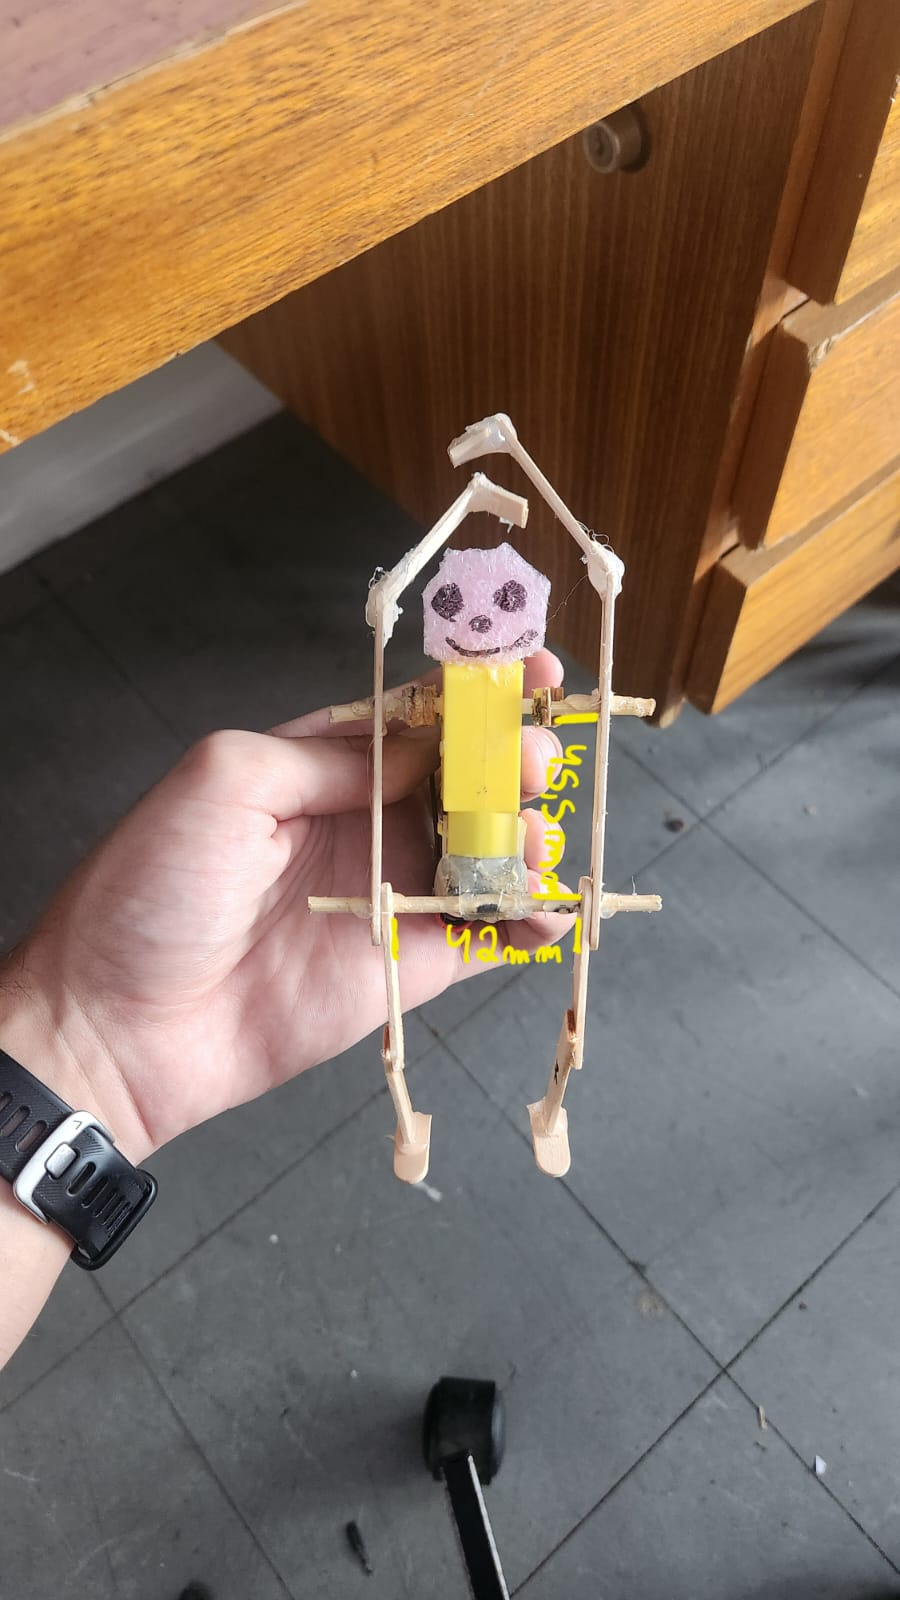
\includegraphics[height=10cm]{foto_robo_montado.jpeg}
\caption{\label{fig:frontal}- Vista frontal do protótipo montado, com as cotas de 42 mm e 45,5 mm.}
\end{center}
\end{figure}

A \ref{fig:robo_montado} mostra a montagem nas vistas frontal e lateral, para a posição da manivela $\psi = 0^\circ$ (pinos no nível do eixo do motor), e a \ref{tab:instancias} lista a massa e o centro de massa de cada peça no sistema do corpo.

\begin{figure}[H]
\begin{center}
 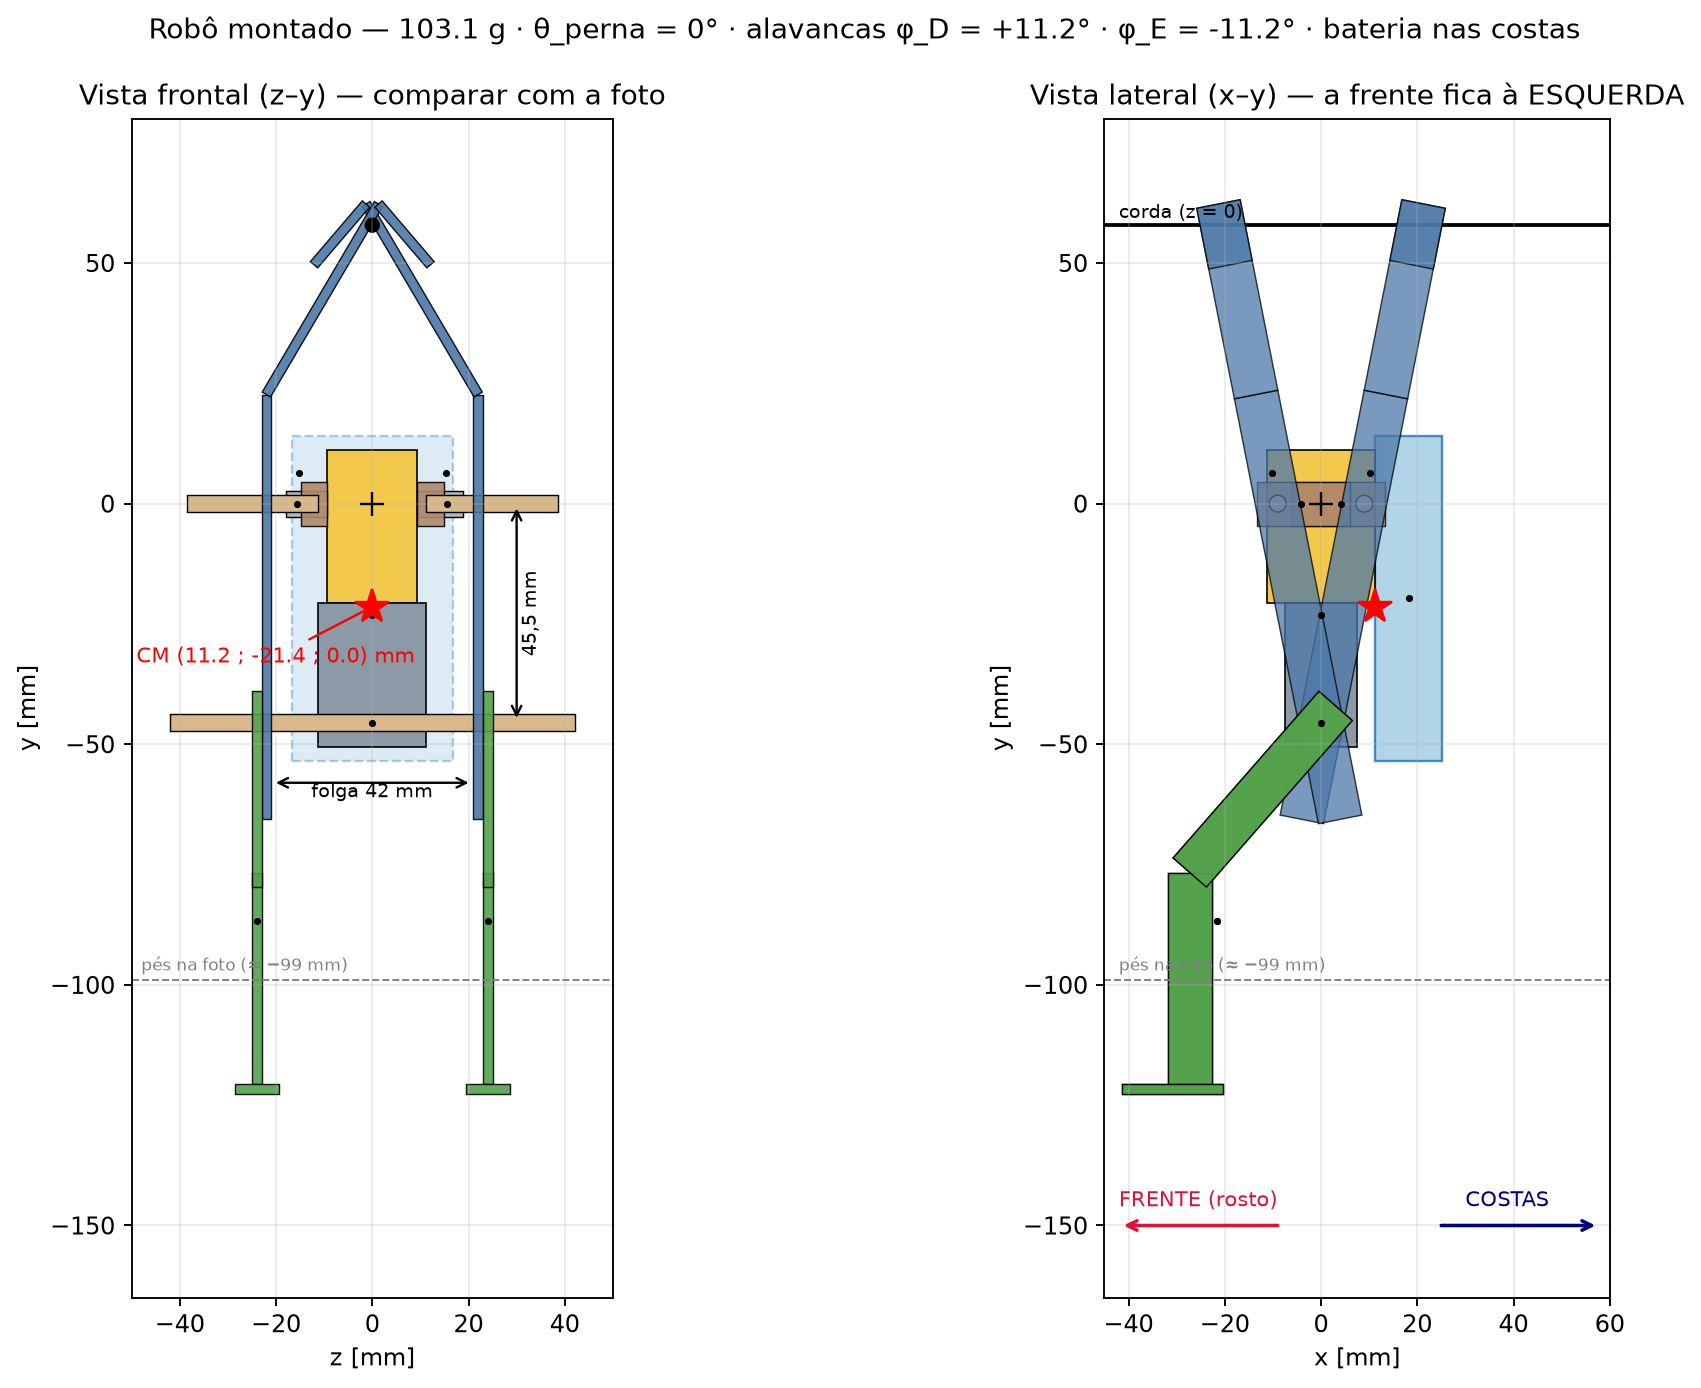
\includegraphics[width=15cm]{robo.png}
\caption{\label{fig:robo_montado}- Robô montado, nas vistas frontal e lateral (a frente fica à esquerda na vista lateral).}
\end{center}
\end{figure}

\begin{table}[H]
\centering
\caption{\label{tab:instancias}- Massa e centro de massa de cada peça no sistema do corpo (posição $\psi=0^\circ$).}
\vspace*{.1cm}
\begin{tabular}{|l|c|c|c|c|}
\hline
\textbf{Peça} & \textbf{Massa (g)} & \textbf{$x_{cm}$ (mm)} & \textbf{$y_{cm}$ (mm)} & \textbf{$z_{cm}$ (mm)} \\
\hline
Motor com caixa de redução & 26,60 & 0,00 & $-$23,18 & 0,01 \\
\hline
Quadril & 0,81 & 0,00 & $-$45,50 & 0,00 \\
\hline
Ombro D & 0,83 & 4,09 & 0,00 & 15,58 \\
\hline
Ombro E & 0,83 & $-$4,09 & 0,00 & $-$15,58 \\
\hline
Braço D & 2,00 & 10,27 & 6,44 & 15,32 \\
\hline
Braço E & 2,00 & $-$10,27 & 6,44 & $-$15,32 \\
\hline
Perna D & 1,50 & $-$21,65 & $-$86,71 & 24,00 \\
\hline
Perna E & 1,50 & $-$21,65 & $-$86,71 & $-$24,00 \\
\hline
Bateria & 67,03 & 18,20 & $-$19,70 & 0,00 \\
\hline
\end{tabular}
\end{table}

O robô completo, com a bateria, tem massa de 103,1 g e centro de massa em (11{,}20; -21{,}42; 0) mm, ou seja, 21,4 mm abaixo do eixo do motor e 11,2 mm atrás dele. O tensor de inércia em torno do centro de massa e os momentos principais são:

\begin{equation*}
[I^*_{\text{robô}}] = \begin{bmatrix}70904{,}3 & -7029{,}3 & -517{,}6 \\
-7029{,}3 & 24957{,}8 & -6{,}9 \\
-517{,}6 & -6{,}9 & 73105{,}0
\end{bmatrix}\ \text{g}\cdot\text{mm}^2, \qquad \text{principais: } 23906; 71761; 73299\ \text{g}\cdot\text{mm}^2.
\end{equation*}

\noindent Em torno do centro do eixo de saída do motor (ponto $O$), o tensor vale

\begin{equation*}
[I_{O,\text{robô}}] = \begin{bmatrix}118210 & 17711 & -521 \\
17711 & 37897 & 0 \\
-521 & 0 & 133349
\end{bmatrix}\ \text{g}\cdot\text{mm}^2.
\end{equation*}

\noindent O tensor depende da posição da manivela, pois os braços inclinam-se alternadamente; os valores acima correspondem a $\psi=0^\circ$. O motor e a bateria respondem por 91\,\% da massa, o que explica a posição baixa do centro de massa e o fato de os produtos de inércia serem pequenos frente aos momentos principais.

\section{Momentos de Inércia dos Corpos Móveis em Torno dos Pivôs}
\label{sec:corpos_moveis}

Como o movimento ocorre no plano $x$--$y$, a dinâmica depende apenas do momento de inércia em torno de eixos paralelos a $z$. Esse momento independe do ângulo de rotação em torno de $z$ e foi calculado para cada corpo móvel em torno do seu pivô por $I_{piv\hat{o}} = I^*_{zz} + m\,d^2$ (Seção \ref{sec:composicao}). A \ref{tab:corpos} reúne os resultados, que são os dados de entrada do modelo dinâmico do Capítulo \ref{chapter:modelo}.

\begin{table}[H]
\centering
\caption{\label{tab:corpos}- Corpos móveis do modelo dinâmico: massa, momento de inércia no centro de massa e em torno do pivô.}
\vspace*{.1cm}
\small
\begin{tabular}{|l|c|c|c|c|}
\hline
\textbf{Corpo} & \textbf{Massa (g)} & \textbf{$I^*_{zz}$ (g$\cdot$mm$^2$)} & \textbf{Pivô} & \textbf{$I_{piv\hat{o}}$ (g$\cdot$mm$^2$)} \\
\hline
Manivela D & 0,83 & 28,8 & eixo do motor & 42,7 \\
\hline
Manivela E & 0,83 & 28,8 & eixo do motor & 42,7 \\
\hline
Alavanca D (braço) & 2,00 & 3219,0 & eixo do quadril & 8825,0 \\
\hline
Alavanca E (braço) & 2,00 & 3219,0 & eixo do quadril & 8825,0 \\
\hline
Perna D & 1,50 & 1220,2 & eixo do quadril & 4471,2 \\
\hline
Perna E & 1,50 & 1220,2 & eixo do quadril & 4471,2 \\
\hline
Chassi (motor, quadril e bateria) & 94,44 & 42812 & --- & --- \\
\hline
\end{tabular}
\end{table}

O chassi reúne o motor com a caixa de redução, o quadril e a bateria e tem centro de massa em (12{,}92; -20{,}90; 0) mm. As alavancas têm inércia em torno do quadril 2,7 vezes maior que a própria ($I_{piv\hat{o}}/I^*_{zz}$) porque seu centro de massa fica a cerca de 52 mm do eixo; nas pernas, essa razão é de 3,7.

\chapter{MODELO CINEMÁTICO E DINÂMICO}
\label{chapter:modelo}

Este capítulo descreve o modelo do mecanismo do robô e o equacionamento do seu movimento. Parte-se da cinemática da manivela e das alavancas, que é prescrita pelo motor, constrói-se a cadeia de referenciais com as equações de velocidade e aceleração do Capítulo \ref{chapter:revisao} e obtêm-se as equações de movimento pela formulação de Newton-Euler projetada nas velocidades generalizadas. O contato dos ganchos com a corda é introduzido por restrições, e a troca de mão por impacto.

\section{Descrição do Mecanismo}
\label{sec:mecanismo}

O eixo de saída do motor atravessa a caixa de redução e recebe um ombro em cada lado (\ref{fig:robo_montado}). Cada ombro é uma manivela cujo pino, paralelo ao eixo e a $R=9{,}0$ mm dele, atravessa uma fenda no braço do mesmo lado. Os braços são hastes rígidas que giram em torno do eixo do quadril, situado $h=45{,}5$ mm abaixo do eixo do motor, e terminam em ganchos que se apoiam na corda. As pernas também giram em torno do quadril, mas livremente, como pêndulos que atuam como contrapesos. Como os pinos das duas manivelas estão defasados de 180$^\circ$, quando um braço se move para trás o outro se move para a frente, e a mão que está apoiada na corda arrasta o robô no sentido oposto ao do seu movimento em relação ao corpo.

\section{Hipóteses e Graus de Liberdade}
\label{sec:hipoteses}

O modelo adota as seguintes hipóteses:

\begin{itemize}
    \item todos os corpos são rígidos e de densidade uniforme (Capítulo \ref{chapter:inercia});
    \item o movimento é plano, no plano $x$--$y$ (sagital): as alavancas e as pernas giram em torno de eixos paralelos a $z$ e o robô é aproximadamente simétrico em $z$, de modo que a rolagem em torno da corda não é considerada;
    \item a manivela gira com velocidade angular constante $\dot\psi = \omega = 30$ rpm $=\pi$ rad/s no sentido anti-horário, de modo que $\psi(t)=\psi_0+\omega t$ (a dinâmica do motor não é modelada);
    \item o pino desliza numa fenda ao longo do braço, de modo que o eixo do braço passa sempre pelo pino (sem a fenda, a distância entre o pino e o quadril, que varia de 36,5 mm a 54,5 mm, não seria compatível com um braço rígido);
    \item a mão engatada na corda é um pino em um ponto da corda, que é suposta reta, horizontal e rígida ($y=0$);
    \item o atrito é representado por amortecimento viscoso nos quadris das pernas e na arfagem do chassi, com coeficientes supostos.
\end{itemize}

Os graus de liberdade do modelo são a posição e a rotação do chassi no plano, ou seja, $x_O$, $y_O$ e $\theta$, e os ângulos das pernas em relação ao chassi, $\theta_D$ e $\theta_E$:
\begin{equation}
    \mathbf{q} = [\,x_O,\; y_O,\; \theta,\; \theta_D,\; \theta_E\,]^T .
    \label{eq:coordenadas}
\end{equation}
A manivela ($\psi$) e as alavancas ($\varphi_D$, $\varphi_E$) têm movimento relativo ao chassi prescrito por $t$ e não contribuem com graus de liberdade, mas suas massas e inércias participam das equações como corpos em movimento prescrito.

\section{Cinemática da Manivela e das Alavancas}
\label{sec:alavancas}

O pino da manivela é um ponto $P$ de um corpo que gira em torno de um ponto $O$ fixo no chassi. Tomando $E\equiv O$ nas Equações \ref{eq:velocidade} e \ref{eq:aceleracao}, com $\vec{v}_{rel}=\vec{0}$ e $\vec{a}_{rel}=\vec{0}$ (o pino pertence ao corpo da manivela), com o chassi parado e $\vec\alpha=\vec 0$:
\begin{equation}
    \vec{v}_P = \vec{\omega}\times\vec{r}_{P/O}, \qquad
    \vec{a}_P = \vec{\omega}\times(\vec{\omega}\times\vec{r}_{P/O}) = -\,\omega^{2}\,\vec{r}_{P/O},
    \label{eq:pino}
\end{equation}
com $\vec r_{P/O}=R(\cos\psi\,\hat{x}+\sin\psi\,\hat{y})$. Para $\omega=\pi$ rad/s e $R=9$ mm, obtêm-se $|\vec v_P| = \omega R = 28,3$ mm/s e $|\vec a_P| = \omega^2 R = 0,089$ m/s$^2$.

O braço D passa pelo pino da manivela D e gira em torno do quadril $H$, situado a $h$ abaixo de $O$. Definindo $\varphi$ como o ângulo do eixo do braço com a vertical, positivo quando o topo vai para trás ($+x$), a condição de o eixo do braço passar pelo pino fornece
\begin{equation}
    \tan\varphi_D = \frac{R\cos\psi}{h + R\sin\psi}
    \quad\Rightarrow\quad
    \varphi_D(\psi)=\operatorname{atan2}\!\big(R\cos\psi,\;h+R\sin\psi\big),
    \qquad \varphi_E(\psi)=\varphi_D(\psi+\pi),
    \label{eq:phi}
\end{equation}
em que o pino E está $180^\circ$ adiante. Derivando em relação a $\psi$:
\begin{equation}
    \frac{d\varphi_D}{d\psi} = -\,\frac{R\,(R + h\sin\psi)}{R^{2}+h^{2}+2Rh\sin\psi},
    \qquad \dot\varphi = \frac{d\varphi}{d\psi}\,\dot\psi,
    \qquad \ddot\varphi = \frac{d^{2}\varphi}{d\psi^{2}}\,\dot\psi^{2}.
    \label{eq:dphi}
\end{equation}
O ângulo da alavanca é máximo quando o pino é tangente ao braço, o que ocorre para $\sin\psi=-R/h$ e dá $\varphi_{max}=\arcsin(R/h) = 11,4^\circ$. Para $\psi=0$, $\varphi_D=11,19^\circ$ e $\varphi_E=-11,19^\circ$.

A mão (ápice do gancho) está a $L_m=109{,}9$ mm do quadril, ao longo do eixo do braço. Em relação ao chassi, seu curso horizontal entre os extremos é $S=L_m(\sin\varphi_{max}-\sin\varphi_{min}) = 2L_mR/h = 43,5$ mm. Se a mão engatada não escorregasse e o chassi não balançasse, o robô avançaria $S$ a cada meia volta da manivela, ou seja, com velocidade média
\begin{equation}
    \bar v_{cin} = 2\,S\,f = \frac{4\,L_m\,R\,f}{h} = 43,5\ \text{mm/s},
    \label{eq:vcin}
\end{equation}
com $f = 0{,}5$ Hz. Esse valor é o limite da cinemática pura e serve de referência para os resultados do Capítulo \ref{chapter:resultados}.

\section{Cadeia de Referenciais}
\label{sec:cadeia}

Adotam-se o referencial inercial $N$ (com $x$ para as costas, $y$ para cima e $z$ perpendicular ao plano do movimento) e, a partir dele, os referenciais do chassi $B$ (girado de $\theta$), das manivelas $C_D$ e $C_E$ (girados de $\psi$ e $\psi+\pi$ em relação a $B$), das alavancas $L_D$ e $L_E$ (girados de $-\varphi_D$ e $-\varphi_E$ em relação a $B$) e das pernas $G_D$ e $G_E$ (girados de $\theta_D$ e $\theta_E$ em relação a $B$). A posição de $O$ é $\vec r_O = x_O\hat x_N + y_O\hat y_N$ e a do quadril é $\vec r_H = \vec r_O + y_h\hat y_B$, com $y_h=-45{,}5$ mm. O centro de massa de cada corpo é fixo no respectivo referencial, a uma distância conhecida do ponto de referência: de $O$, para o chassi e as manivelas, e de $H$, para as alavancas e as pernas. A mão $M_j$ ($j=D,E$) é o ponto da alavanca a $L_m$ do quadril:
\begin{equation}
    \vec{r}_{M_j} = \vec r_O + y_h\,\hat{y}_B + L_m\left(\sin\varphi_j\,\hat{x}_B + \cos\varphi_j\,\hat{y}_B\right).
    \label{eq:mao}
\end{equation}

Para cada corpo, a velocidade e a aceleração do centro de massa são obtidas pelas Equações \ref{eq:velocidade} e \ref{eq:aceleracao} tomando um ponto de referência $E$ do mesmo corpo rígido (de modo que $\vec v_{rel}=\vec a_{rel}=\vec 0$), com a velocidade angular absoluta do corpo, por exemplo $\omega_{L_j}=\dot\theta-\dot\varphi_j$ para as alavancas e $\omega_{C_j}=\dot\theta+\dot\psi$ para as manivelas, e com a velocidade e a aceleração do ponto de referência obtidas do corpo anterior da cadeia (do chassi, para $O$ e $H$). O movimento relativo entre corpos aparece, assim, na velocidade e na aceleração angulares absolutas de cada corpo e na aceleração do ponto de referência. A mesma cadeia fornece $\vec\alpha$ e $\vec\omega$ de cada corpo para a equação de Euler.

\section{Equações de Movimento}
\label{sec:eqmov}

Para cada um dos sete corpos ($i=1,\dots,7$: chassi, duas manivelas, duas alavancas e duas pernas), valem as equações de Newton e de Euler (Equações \ref{eq:newton} e \ref{eq:euler_momentos}). No movimento plano, o tensor de inércia entra apenas pelo momento $I_{zz,i}$ em torno do eixo $z$ que passa pelo centro de massa, e a equação de Euler se reduz a $\dot{H}_{z,i}=I_{zz,i}\,\alpha_{i}+\left[\vec\omega_i\times(\left[I_i\right]\vec\omega_i)\right]_z = I_{zz,i}\,\alpha_i$, pois o termo giroscópico é perpendicular ao plano e não afeta o movimento plano. Projetando as duas equações nas velocidades parciais dos corpos em relação às velocidades generalizadas $\dot q_k$ (método de Kane \cite{kane1985}), eliminam-se as reações internas que não realizam trabalho, e resulta para $k=1,\dots,5$:
\begin{equation}
    \sum_{i=1}^{7}\Big[\big(m_i\,\vec a_i-\vec F_i\big)\cdot\frac{\partial\vec v_i}{\partial\dot q_k}
    +\big(I_{zz,i}\,\alpha_i-M_{z,i}\big)\frac{\partial\omega_i}{\partial\dot q_k}\Big]=0,
    \label{eq:kane}
\end{equation}
em que $\vec F_i = -m_i g\,\hat y_N$ é o peso e $M_{z,i}$ inclui os amortecimentos, que entram como forças generalizadas $Q_\theta=-c_{ch}\dot\theta$ e $Q_{\theta_j}=-c_{p}\dot\theta_j$. Como as velocidades e as acelerações são lineares nas acelerações generalizadas, a Equação \ref{eq:kane} resulta em
\begin{equation}
    \mathbf{M}(\mathbf{q},t)\,\ddot{\mathbf{q}} + \mathbf{c}(\mathbf{q},\dot{\mathbf{q}},t) = \mathbf{A}^{T}\boldsymbol{\lambda},
    \qquad
    M_{kl}=\sum_i\Big[m_i\frac{\partial\vec v_i}{\partial\dot q_k}\cdot\frac{\partial\vec v_i}{\partial\dot q_l}+I_{zz,i}\frac{\partial\omega_i}{\partial\dot q_k}\frac{\partial\omega_i}{\partial\dot q_l}\Big],
    \label{eq:Mqdd}
\end{equation}
em que $\mathbf{M}$ é a matriz de massa, $\mathbf{c}$ reúne os termos de velocidade, o peso e o efeito do movimento prescrito de $\psi$ e das alavancas, e $\mathbf{A}^T\boldsymbol{\lambda}$ é a força da corda sobre o gancho.

\section{Contato com a Corda, Troca de Mão e Impacto}
\label{sec:contato}

Quando a mão $j$ está engatada, seu ponto $\vec{r}_{M_j}$ coincide com um ponto fixo da corda, $\vec{r}_c$:
\begin{equation}
    \mathbf{g}(\mathbf{q},t)=\vec r_M(\mathbf{q},t)-\vec r_c=\mathbf{0}
    \;\Rightarrow\;
    \mathbf{A}\ddot{\mathbf q}+\mathbf b=\mathbf 0,
    \label{eq:restricao}
\end{equation}
em que $\mathbf A=\partial\mathbf g/\partial\mathbf q$ e $\mathbf b=\frac{d^2\mathbf g}{dt^2}$ com $\ddot{\mathbf q}=0$ (não nulo, pois a mão se move em relação ao chassi enquanto a manivela gira). As Equações \ref{eq:Mqdd} e \ref{eq:restricao} formam o sistema linear
\begin{equation}
    \begin{bmatrix}\mathbf{M} & -\mathbf{A}^{T}\\ \mathbf{A} & \mathbf 0\end{bmatrix}
    \begin{bmatrix}\ddot{\mathbf q}\\ \boldsymbol\lambda\end{bmatrix}
    =
    \begin{bmatrix}-\mathbf c\\ -\mathbf b-2\xi\omega_n\dot{\mathbf g}-\omega_n^{2}\mathbf g\end{bmatrix},
    \label{eq:kkt}
\end{equation}
em que os dois últimos termos do lado direito são a estabilização de Baumgarte \cite{baumgarte1972}, com $\xi=1$ e $\omega_n=60$ s$^{-1}$, que impede a deriva numérica da restrição. O vetor $\boldsymbol\lambda=(\lambda_x,\lambda_y)$ é a força da corda sobre o gancho; como a corda só pode sustentar o robô, exige-se $\lambda_y>0$.

A mão engatada é escolhida pela fase da manivela. A mão desejada é a E quando $\sin\psi>0$ e a D quando $\sin\psi<0$, o que alterna a cada meia volta; e essa regra, com a manivela girando no sentido anti-horário, faz o robô avançar para a frente. Ao mudar a mão desejada, a nova mão só engata quando sua ponta sobe até a altura da corda ($y=0$, cruzando de baixo para cima), pois um gancho aberto para baixo apanha a corda por baixo; nesse instante, o gancho anterior se solta. A mão que engata para, em relação à corda, de forma abrupta; trata-se de um impacto perfeitamente plástico, com impulso $\boldsymbol\Lambda$ no ponto de contato, que modifica as velocidades generalizadas de $\dot{\mathbf q}^-$ para $\dot{\mathbf q}^+$ sem alterar as posições:
\begin{equation}
    \mathbf{M}\,(\dot{\mathbf q}^{+}-\dot{\mathbf q}^{-}) = \mathbf{A}^{T}\boldsymbol\Lambda,
    \qquad
    \mathbf{A}\,\dot{\mathbf q}^{+} = \mathbf 0 .
    \label{eq:impacto}
\end{equation}

\section{Integração Numérica, Condições Iniciais e Verificação}
\label{sec:numerica}

As matrizes e vetores das Equações \ref{eq:Mqdd} e \ref{eq:restricao} foram obtidos simbolicamente com a biblioteca SymPy \cite{sympy2017} e integrados com o método de Runge-Kutta de ordem 4(5) de Dormand-Prince \cite{dormand1980}, da biblioteca SciPy \cite{scipy2020}, com tolerâncias relativa de $10^{-8}$ e absoluta de $10^{-10}$ e passo máximo de 5 ms, com detecção do evento de engate da corda. A cada passo, o sistema linear da Equação \ref{eq:kkt} é resolvido para $\ddot{\mathbf q}$ e $\boldsymbol\lambda$. A violação máxima da restrição da corda durante toda a simulação foi de 0,079 mm.

A condição inicial é o equilíbrio estático do robô pendurado pela mão E em $\psi_0=0$, com velocidades nulas, obtido pela minimização da energia potencial em relação a $\theta$, $\theta_D$ e $\theta_E$. O resultado é $\theta=$-$21,9^\circ$ (arfagem do chassi) e ângulo das pernas em relação ao chassi de 49,6$^\circ$, ou seja, 27,7$^\circ$ em relação à posição do desenho da \ref{fig:perna_modelo}.

Para verificar o equacionamento, as equações obtidas pela projeção de Newton-Euler foram comparadas com as equações de Lagrange do mesmo sistema, $\frac{d}{dt}\frac{\partial T}{\partial\dot q_k}-\frac{\partial T}{\partial q_k}+\frac{\partial V}{\partial q_k}=Q_k$, em cinco estados aleatórios. A diferença relativa máxima entre os dois resíduos foi de $1{,}7\cdot 10^{-16}$, ou seja, coincidem até o erro de arredondamento.

A \ref{tab:param_dyn} reúne os valores adotados no modelo dinâmico.

\begin{table}[H]
\centering
\caption{\label{tab:param_dyn}- Parâmetros do modelo dinâmico.}
\vspace*{.1cm}
\begin{tabular}{|l|c|}
\hline
\textbf{Parâmetro} & \textbf{Valor} \\
\hline
Velocidade da manivela ($\omega$) & 30 rpm ($\pi$ rad/s), anti-horário \\
\hline
Raio da manivela ($R$) & 9,0 mm \\
\hline
Distância eixo do motor -- quadril ($h$) & 45,5 mm \\
\hline
Distância quadril -- ápice da mão ($L_m$) & 109,9 mm \\
\hline
Massa total do robô & 103,1 g \\
\hline
Amortecimento da arfagem do chassi ($c_{ch}$) & $10^{-4}$ N$\cdot$m$\cdot$s/rad (suposto) \\
\hline
Amortecimento dos quadris ($c_{p}$) & $5\cdot 10^{-5}$ N$\cdot$m$\cdot$s/rad (suposto) \\
\hline
Gravidade ($g$) & 9,81 m/s$^2$ \\
\hline
Duração da simulação & 8 s \\
\hline
\end{tabular}
\end{table}

\chapter{RESULTADOS E DISCUSSÃO}
\label{chapter:resultados}

Este capítulo apresenta os resultados da simulação do robô com o motor a 30 rpm no sentido anti-horário, durante 8 s, para o modelo do Capítulo \ref{chapter:modelo} com os parâmetros inerciais do Capítulo \ref{chapter:inercia}. Os pontos escolhidos para acompanhar o deslocamento são o centro de massa do robô e a ponta superior de cada braço (a mão).

\section{Movimento das Alavancas}
\label{sec:res_alavancas}

A \ref{fig:alavancas_res} mostra o ângulo das duas alavancas e suas derivadas ao longo de uma volta da manivela (2 s), calculados pelas Equações \ref{eq:phi} e \ref{eq:dphi}. Os braços oscilam em oposição de fase entre $-11,4^\circ$ e $+11,4^\circ$, com velocidade angular máxima de 0,77 rad/s e aceleração angular máxima de 2,34 rad/s$^2$. O movimento não é senoidal puro: a fenda e o pino fazem com que o curso em um sentido dure mais que no outro (cerca de 203$^\circ$ de manivela contra 157$^\circ$).

\begin{figure}[H]
\begin{center}
 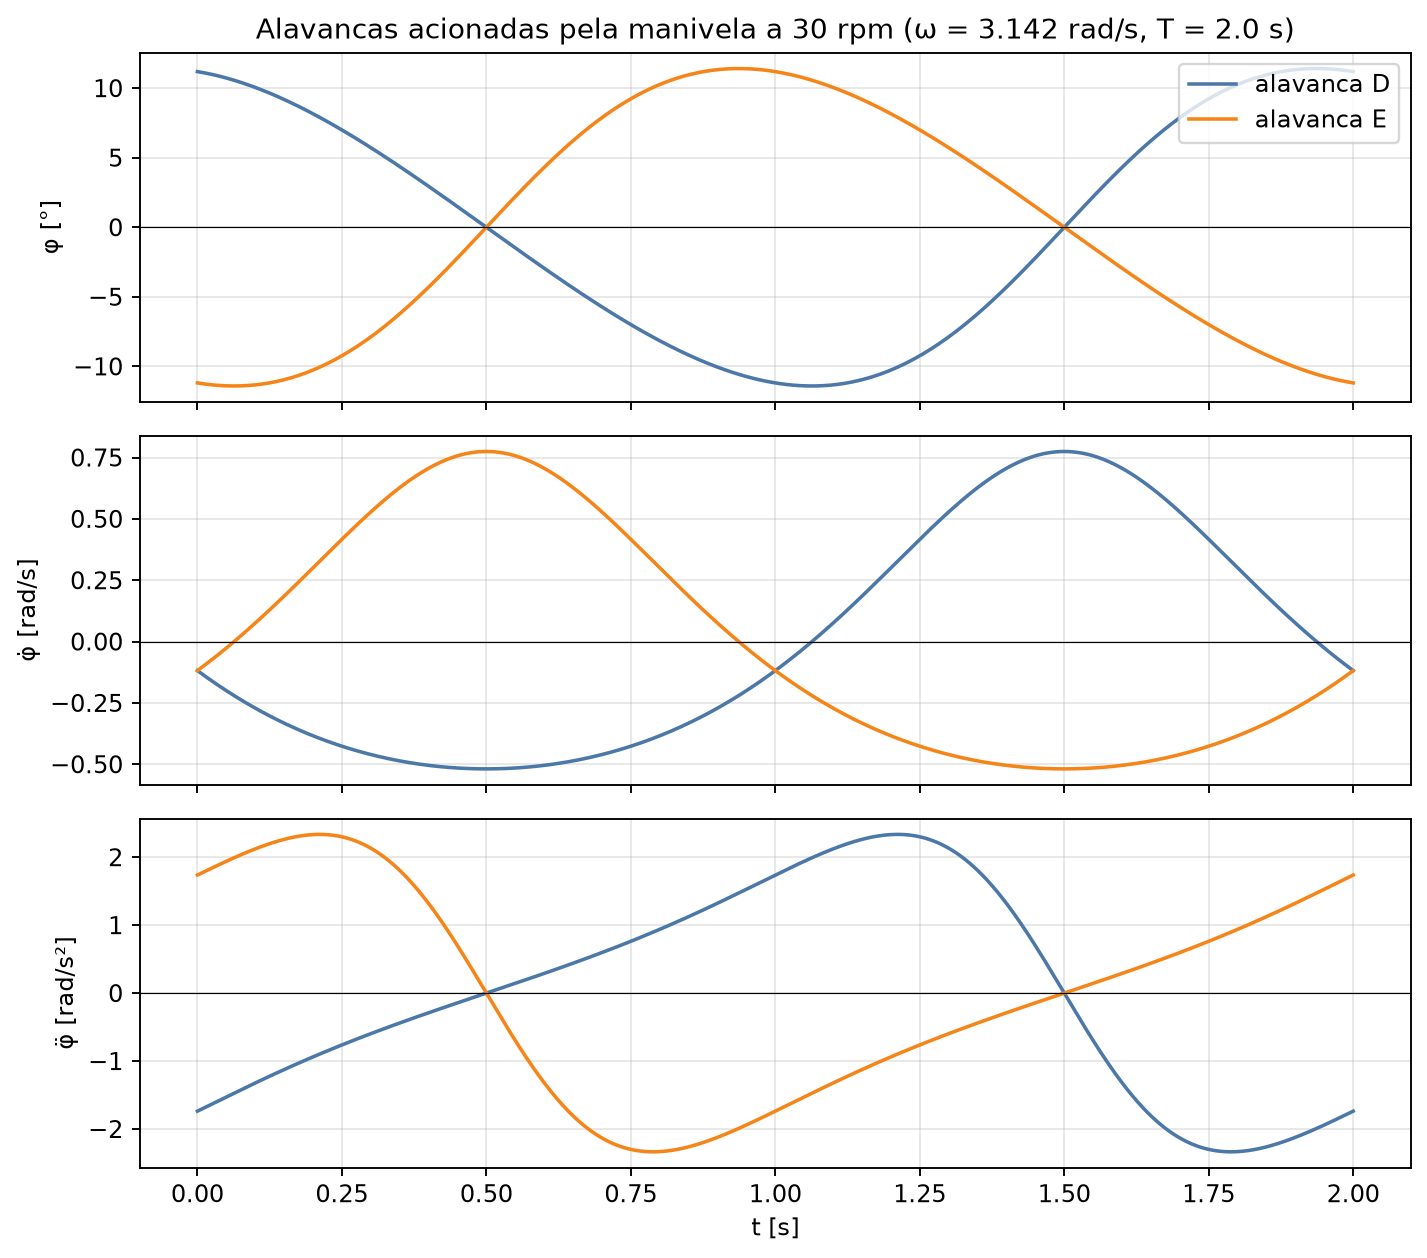
\includegraphics[width=12.5cm]{alavancas.png}
\caption{\label{fig:alavancas_res}- Ângulo, velocidade angular e aceleração angular das alavancas D e E para a manivela a 30 rpm.}
\end{center}
\end{figure}

\section{Deslocamento do Centro de Massa e das Mãos}
\label{sec:res_deslocamento}

A \ref{fig:deslocamento_res} mostra o avanço do centro de massa e da ponta das duas mãos, positivo para a frente, comparado com a reta da cinemática pura (Equação \ref{eq:vcin}), além dos ângulos do chassi e das pernas e da força vertical da corda sobre o gancho engatado. As linhas pontilhadas marcam as trocas de mão, listadas na \ref{tab:trocas}. Os valores numéricos da simulação estão reunidos na \ref{tab:resultados}.

\begin{figure}[H]
\begin{center}
 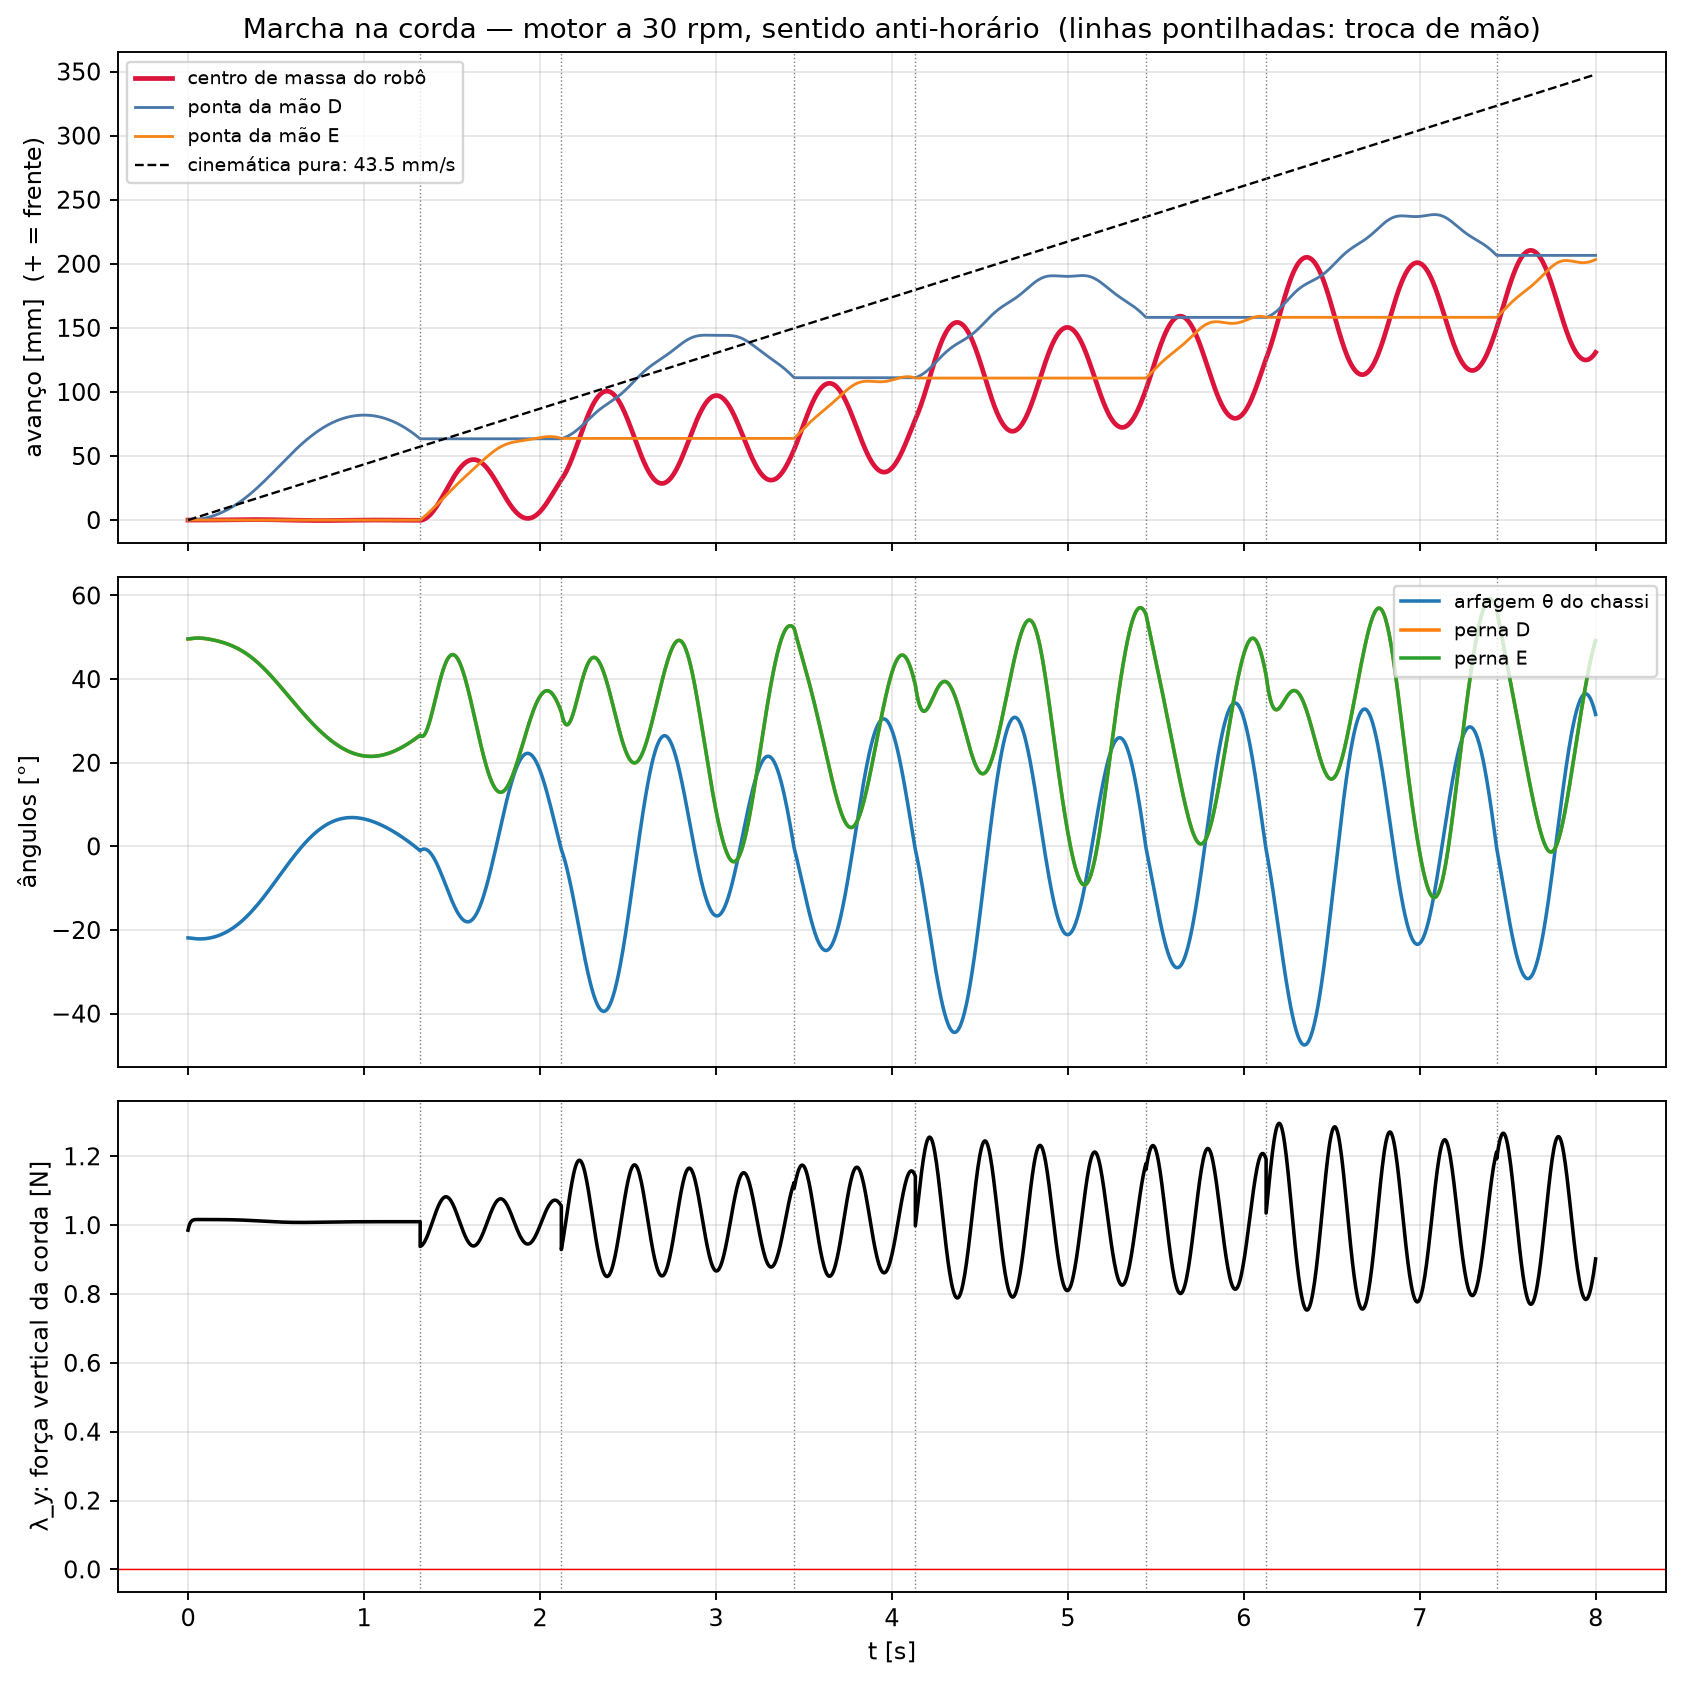
\includegraphics[width=14cm]{deslocamento.png}
\caption{\label{fig:deslocamento_res}- Avanço do centro de massa e das mãos, ângulos do chassi e das pernas e força vertical da corda ($c_{ch}=10^{-4}$ N$\cdot$m$\cdot$s/rad).}
\end{center}
\end{figure}

\begin{table}[H]
\centering
\caption{\label{tab:resultados}- Resultados da simulação (8 s, 30 rpm, anti-horário).}
\vspace*{.1cm}
\begin{tabular}{|l|c|}
\hline
\textbf{Grandeza} & \textbf{Valor} \\
\hline
Avanço do centro de massa & 130,8 mm \\
\hline
Avanço da ponta da mão D & 206,5 mm \\
\hline
Avanço da ponta da mão E & 203,3 mm \\
\hline
Velocidade média na última volta & 22,6 mm/s \\
\hline
Limite da cinemática pura & 43,5 mm/s \\
\hline
Razão entre as duas velocidades & 52\,\% \\
\hline
Variação da altura do centro de massa & 18,0 mm \\
\hline
Arfagem máxima do chassi & 47,5$^\circ$ \\
\hline
Ângulo máximo das pernas em relação ao chassi & 59,2$^\circ$ \\
\hline
Força vertical da corda sobre o gancho & de 0,75 a 1,30 N (peso: 1,01 N) \\
\hline
Número de trocas de mão & 7 \\
\hline
Energia máxima dissipada em um impacto & 1,5 mJ \\
\hline
\end{tabular}
\end{table}

O centro de massa avançou 130,8 mm em 8 s e as mãos avançaram 206,5 mm e 203,3 mm, de modo que o robô caminha para a frente, como esperado para a manivela no sentido anti-horário. A velocidade média na última volta foi de 22,6 mm/s, cerca de 52\,\% do limite da cinemática pura (43,5 mm/s). Esse limite supõe que o chassi não balança e que cada mão engata assim que a anterior termina o curso; na simulação, o gancho só engata quando sua ponta sobe até a corda, o que ocorre de 0,1 s a 0,4 s depois do instante em que a fase da manivela troca a mão desejada (\ref{tab:trocas}), e esse atraso, mais o curso perdido em cada espera, reduz a velocidade média.

\begin{table}[H]
\centering
\caption{\label{tab:trocas}- Trocas de mão: instante do engate, mão que engata, instante da troca da mão desejada, atraso e energia dissipada no impacto.}
\vspace*{.1cm}
\begin{tabular}{|c|c|c|c|c|}
\hline
\textbf{Engate (s)} & \textbf{Mão} & \textbf{Troca desejada (s)} & \textbf{Atraso (s)} & \textbf{Energia (mJ)} \\
\hline
1,32 & D & 1,00 & 0,32 & $-$0,01 \\
\hline
2,12 & E & 2,00 & 0,12 & 0,41 \\
\hline
3,44 & D & 3,00 & 0,44 & 0,00 \\
\hline
4,13 & E & 4,00 & 0,13 & 1,06 \\
\hline
5,44 & D & 5,00 & 0,44 & 0,02 \\
\hline
6,13 & E & 6,00 & 0,13 & 1,47 \\
\hline
7,44 & D & 7,00 & 0,44 & 0,05 \\
\hline
\end{tabular}
\end{table}

O mecanismo do avanço pode ser lido na \ref{fig:deslocamento_res}. Enquanto o robô está pendurado por uma mão, o centro de massa tende a ficar logo abaixo do gancho (equilíbrio do pêndulo), de modo que o curso do braço em relação ao chassi apenas altera a arfagem. É na troca de mão que o avanço ocorre: o novo gancho engata, em média, cerca de $S=43,5$ mm à frente na corda (curso da mão em relação ao chassi), e o robô balança para a frente sob a ação da gravidade em direção ao novo equilíbrio. Isso explica o aspecto em degraus da curva da mão e o balanço do centro de massa em torno da tendência média.

\section{Trajetórias, Ângulos e Forças}
\label{sec:res_traj}

A \ref{fig:trajetorias_res} mostra as trajetórias do centro de massa e das mãos no plano $x$--$y$. A mão engatada fica sobre a corda, e a mão livre descreve arcos acima e abaixo dela. O centro de massa permanece em média 82 mm abaixo da corda e oscila verticalmente por 18,0 mm. O chassi balança com amplitude de até 47,5$^\circ$ e as pernas, com amplitude de até 59,2$^\circ$ em relação ao chassi, que inclui o ângulo inicial de equilíbrio. A força vertical da corda sobre o gancho engatado variou entre 0,75 N e 1,30 N em torno do peso de 1,01 N e foi sempre positiva, ou seja, a corda nunca precisou empurrar o gancho para baixo, o que é coerente com a hipótese de contato unilateral.

\begin{figure}[H]
\begin{center}
 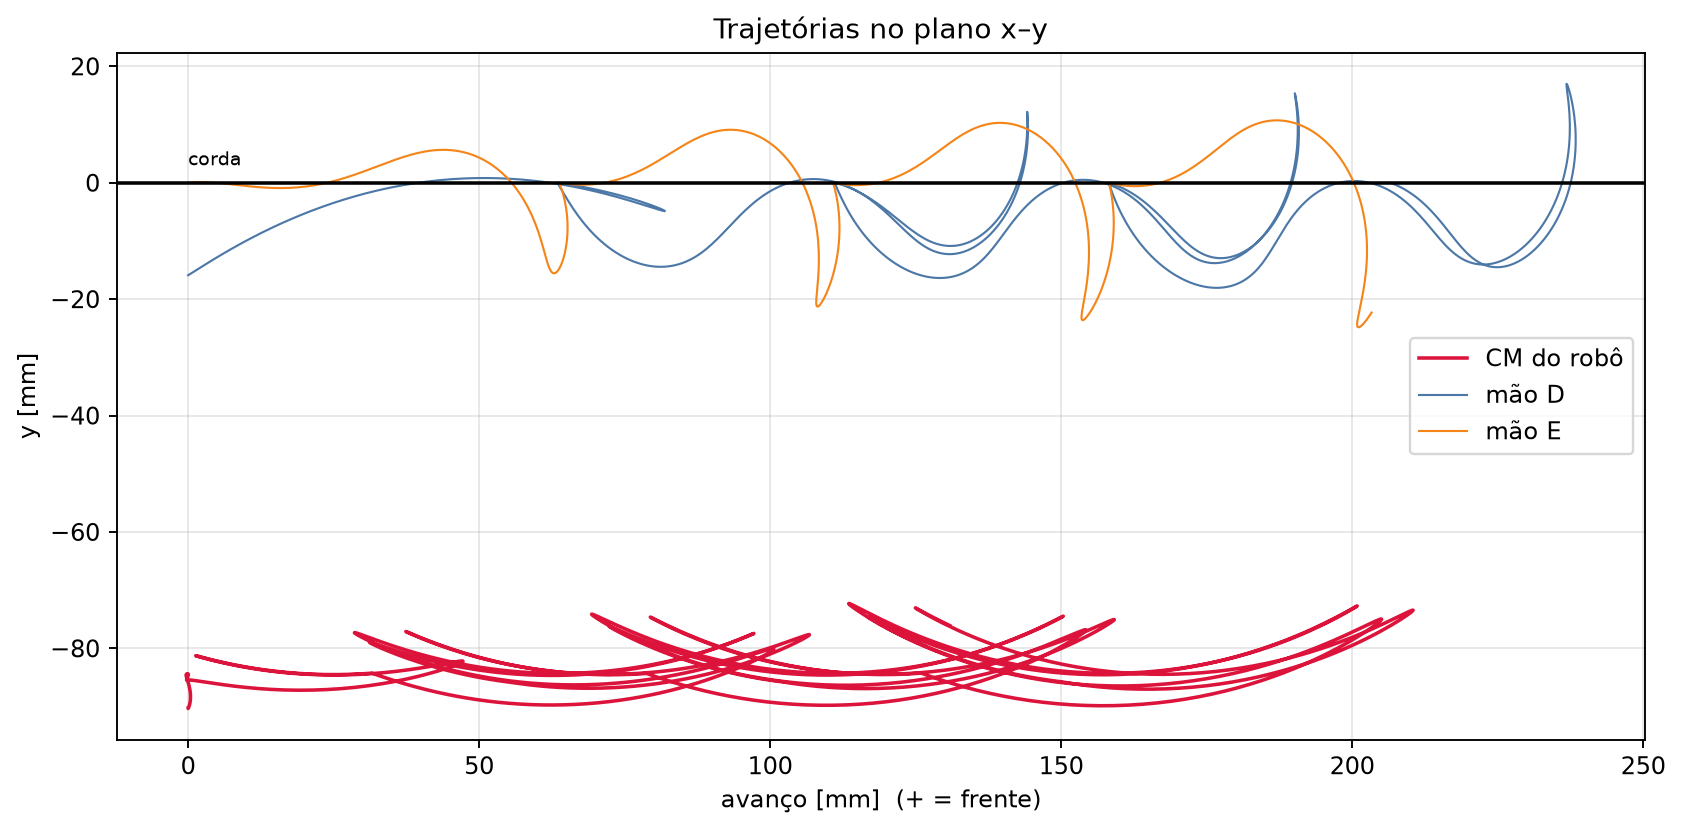
\includegraphics[width=14cm]{trajetorias.png}
\caption{\label{fig:trajetorias_res}- Trajetórias do centro de massa e das mãos no plano $x$--$y$ (a corda é a reta $y=0$).}
\end{center}
\end{figure}

\section{Sensibilidade ao Amortecimento}
\label{sec:sensibilidade}

O amortecimento da arfagem do chassi ($c_{ch}$) e dos quadris ($c_p$) não foi medido e foi suposto. A \ref{tab:sens} mostra o efeito de variá-los. O sentido do movimento (para a frente) e a ordem de grandeza do avanço se mantêm em todos os casos, mas o valor varia de 127 mm a 218 mm em 8 s. A variação não é monotônica, pois o avanço depende de quando cada gancho alcança a corda: pequenas mudanças na dinâmica deslocam o instante do engate e, com ele, o número de trocas completadas. Para $c_{ch}$ de 0 a $5\cdot 10^{-4}$ N$\cdot$m$\cdot$s/rad o resultado é estável (127 a 131 mm), e o amortecimento dos quadris pouco influencia o avanço do centro de massa.

\begin{table}[H]
\centering
\caption{\label{tab:sens}- Sensibilidade do avanço do centro de massa em 8 s e da velocidade média na última volta aos coeficientes de amortecimento.}
\vspace*{.1cm}
\begin{tabular}{|c|c|c|c|}
\hline
\textbf{$c_{ch}$ (N$\cdot$m$\cdot$s/rad)} & \textbf{$c_p$ (N$\cdot$m$\cdot$s/rad)} & \textbf{Avanço (mm)} & \textbf{Velocidade (mm/s)} \\
\hline
0 & $5\cdot 10^{-5}$ & 127,3 & 22,3 \\
\hline
$10^{-4}$ (adotado) & $5\cdot 10^{-5}$ & 130,8 & 22,6 \\
\hline
$5\cdot 10^{-4}$ & $5\cdot 10^{-5}$ & 129,1 & 20,4 \\
\hline
$10^{-3}$ & $5\cdot 10^{-5}$ & 218,4 & 41,5 \\
\hline
$1{,}5\cdot 10^{-3}$ & $2\cdot 10^{-5}$ & 194,8 & 20,6 \\
\hline
$1{,}5\cdot 10^{-3}$ & $5\cdot 10^{-5}$ & 200,6 & 22,0 \\
\hline
$1{,}5\cdot 10^{-3}$ & $10^{-4}$ & 203,3 & 22,8 \\
\hline
$3\cdot 10^{-3}$ & $5\cdot 10^{-5}$ & 190,9 & 29,6 \\
\hline
\end{tabular}
\end{table}

\section{Discussão}
\label{sec:discussao}

O resultado principal é que, com os parâmetros inerciais medidos e o motor a 30 rpm no sentido anti-horário, o modelo prevê um avanço do robô para a frente de cerca de 23 mm/s, aproximadamente a metade do limite cinemático de 43,5 mm/s. A velocidade média prevista pode ser comparada diretamente com a obtida das filmagens do protótipo, medindo-se o deslocamento de um ponto marcado (a mão ou o centro de massa) por volta da manivela, que é a validação experimental natural do modelo.

Um resultado independente que dá confiança ao modelo é o ângulo de equilíbrio das pernas: penduradas livremente, elas se afastam de 27,7$^\circ$ da posição do desenho da \ref{fig:perna_modelo}, valor que coincide com o ângulo de aproximadamente 28$^\circ$ que reproduz a altura dos pés observada na vista frontal do protótipo (\ref{fig:frontal}). Isso indica que, na fotografia, as pernas estão apenas penduradas e que o centro de massa da perna foi bem estimado.

As principais limitações são: (i) o modelo é plano e não inclui a rolagem em torno da corda; (ii) o amortecimento foi suposto e influencia o avanço; (iii) a regra de engate (mão desejada pela fase da manivela e engate quando a ponta sobe até a corda) é uma hipótese de modelagem, e não foi derivada da geometria detalhada do gancho; (iv) a massa do motor (26,6 g) foi medida, mas a repartição da massa entre caixa e motor é suposta; (v) as posições do quadril, do furo da perna e da bateria foram estimadas a partir das fotografias; e (vi) o torque do motor não foi calculado, pois a velocidade da manivela foi prescrita. Com os mesmos corpos e as mesmas equações, o torque necessário no eixo pode ser obtido como força generalizada associada a $\psi$, o que permitiria dimensionar o motor.






\pagebreak
\chapter{CONCLUSÃO}
\label{chapter:conclusao}

Este trabalho concluiu o ciclo de projeto mecânico previsto na disciplina de Dinâmica: a fundamentação teórica, a construção do protótipo, o levantamento dos parâmetros físicos e o equacionamento completo do movimento do robô articulado que se desloca sobre uma corda.

A elaboração da modelagem teórica e física do mecanismo articulado demonstrou a importância da padronização dos sistemas de referência e do uso rigoroso das equações vetoriais na engenharia. A utilização das equações de velocidade e aceleração relativa permitiu transcrever a geometria do movimento do robô para uma formulação matemática consistente.

A etapa de levantamento dos parâmetros físicos do protótipo construído com palitos de madeira e motor DC — extraindo massas, dimensões e calculando tensores de inércia por decomposição em sólidos homogêneos e composição pelo teorema dos eixos paralelos — constituiu a base fundamental para a aplicação das leis de Newton e da equação de Euler para a cinética do sistema. O robô montado resultou em 103,1 g, com centro de massa 21,4 mm abaixo do eixo do motor, valores dominados pela bateria e pelo motor com caixa de redução, que somam 91\,\% da massa.

O modelo cinemático e dinâmico, construído pela cadeia de referenciais e pelas equações de Newton-Euler projetadas nas velocidades generalizadas, foi verificado contra a formulação de Lagrange com diferença relativa da ordem de $10^{-16}$. A simulação com o motor a 30 rpm no sentido anti-horário previu um avanço para a frente do centro de massa de 130,8 mm em 8 s (velocidade média de 22,6 mm/s, cerca de 52\,\% do limite da cinemática pura de 43,5 mm/s), com força vertical da corda sempre positiva e trocas de mão por impacto plástico. O mecanismo do avanço — engate do gancho à frente, seguido do balanço pendular do corpo — ficou claramente caracterizado nas trajetórias e nos degraus da curva de deslocamento.

Espera-se que, com o equacionamento matricial e vetorial estabelecido neste relatório, a futura comparação com as filmagens do protótipo valide o deslocamento previsto, e que o cálculo do torque necessário no eixo do motor — obtido como força generalizada associada à rotação da manivela — permita dimensionar o motor e as reações nas juntas de madeira durante a operação, completando o detalhamento dinâmico do projeto.

As principais extensões do trabalho são: medir a massa do motor e o amortecimento real do mecanismo; derivar a regra de engate da geometria precisa do gancho; incluir a rolagem em torno da corda em um modelo espacial; e comparar os ângulos do chassi e das pernas previstos com os medidos nas filmagens do protótipo em operação.


\pagebreak
\addcontentsline{toc}{chapter}{\hspace{1.7cm}\bfseries REFERÊNCIAS}
\def\bibname{REFERÊNCIAS}




% abaixo segue a chamada para o arquivo [.BIB]. Utilizei o programa JABREF para montar o arquivo com minhas referências.
\bibliography{dissertacao}



% ------------------ APÊNDICE ------------------
\pagebreak
\setcounter{chapter}{0}%
\renewcommand{\thechapter}{A}%
\renewcommand{\thesection}{\thechapter.\arabic{section}}%
\chapter{APÊNDICE}
\label{ap:codigo}

O equacionamento do robô foi implementado em Python, no ambiente Jupyter, no notebook \texttt{blocos\_inercia\_robo.ipynb}, organizado em onze blocos cumulativos. A seguir, a estrutura (\ref{tab:blocos}):

\begin{table}[H]
\centering
\caption{\label{tab:blocos}- Estrutura do notebook \texttt{blocos\_inercia\_robo.ipynb}.}
\vspace*{.1cm}
\small
\begin{tabular}{|c|p{11.5cm}|}
\hline
\textbf{Bloco} & \textbf{Conteúdo} \\
\hline
1 & Importações (NumPy, SymPy, Matplotlib) e configuração de exibição. \\
\hline
2 & Funções gerais: exibição de equações em LaTeX, conversão de unidades e funções utilitárias. \\
\hline
3 & Braço: massas, centro de massa e tensor de inércia das três barras, com cálculo simbólico em SymPy. \\
\hline
4 & Perna (contrapeso): mesma rotina do Braço, com desenho cotado da peça. \\
\hline
5 & Ombro: manivela em pilha de camadas, furo passante (massa negativa) e pino cilíndrico. \\
\hline
6 & Motor com caixa de redução: composição do corpo e da caixa a partir do desenho técnico. \\
\hline
7 & Bateria: paralelepípedo homogêneo, verificação de densidade e conversão de unidades. \\
\hline
8 & Quadril: haste fina, comparação entre as hipóteses de seção circular e quadrada. \\
\hline
9 & Montagem do robô completo no sistema do corpo, com a posição ($\psi=0^\circ$) definida na Tabela de dimensões e o desenho das vistas. \\
\hline
10 & Corpos móveis e manivela a 30 rpm: cinemática das alavancas (Equações \ref{eq:phi} e \ref{eq:dphi}) e inércia em torno dos pivôs. \\
\hline
11 & Modelo dinâmico plano: montagem simbólica das matrizes de massa e dos vetores de contato, verificação contra Lagrange, detecção de eventos de engate e integração das equações da marcha na corda. \\
\hline
\end{tabular}
\end{table}





%felipe% \printindex    %Removi o índice remissivo para a versão oficial do trabalho.


\end{document}